\documentclass{book}

\title{Analisi Matematica T-A}
\author{Michele Mazza}
\date{November 2023}


% Pacchetti di Codifica e Lingua
\usepackage[utf8]{inputenc}
\usepackage[T1]{fontenc}
\usepackage[italian]{babel}

% Pacchetti Grafici e Diagrammi
\usepackage{graphicx}
\usepackage{tikz}
\usepackage{tikz-3dplot}
\usetikzlibrary{angles,quotes,arrows.meta, positioning}
\usepackage{pgfplots}
\pgfplotsset{compat=1.18}

% Pacchetti Matematici
\usepackage{amsmath, amssymb, amsthm}

% Pacchetti per Tabelle e Unità di Misura
\usepackage{geometry}
\usepackage{siunitx}
\usepackage{booktabs}
\usepackage{tabularx}
\usepackage{colortbl}

% Pacchetti per Layout e Formattazione
\usepackage{fancyhdr}
\usepackage{float}
\usepackage{microtype}

% Altri Pacchetti Utili
\usepackage{mdframed}
\usepackage{animate}

% Pacchetto enumitem
\usepackage{enumitem}

% Definizioni dei Colori
\definecolor{lightblue}{HTML}{9cd8fc}
\definecolor{myblue}{HTML}{139FE9}

% Definizione del comando \norm
\newcommand{\norm}[1]{\left\lVert#1\right\rVert}

%\font\nullfont=cmr10 

% Ambienti Personalizzati
\newmdtheoremenv[
    backgroundcolor=orange!10,
    linecolor=myblue,
    linewidth=0pt,
    leftmargin=0pt,
    rightmargin=0pt,
    innerleftmargin=10pt,
    innerrightmargin=10pt,
    innertopmargin=10pt,
    innerbottommargin=10pt,
    nobreak
]{curiosity}{Curiosità}

\newmdtheoremenv[
    font=\normalfont\small,
    linewidth=0pt,
    innerleftmargin=10pt,
    innerrightmargin=10pt,
]{example}{Esempio}

\newmdtheoremenv[
  backgroundcolor=lightblue,
  linecolor=myblue,
  linewidth=1.5pt,
  innertopmargin=10pt,
  innerbottommargin=10pt,
  innerrightmargin=10pt,
  innerleftmargin=10pt,
  nobreak
]{theorem}{Teorema}

\newmdtheoremenv[
  backgroundcolor=gray!10,
  linewidth=0pt,
  innertopmargin=10pt,
  innerbottommargin=10pt,
  innerrightmargin=10pt,
  innerleftmargin=10pt,
  nobreak
]{definition}{Definizione}

\newmdtheoremenv[
  backgroundcolor=gray!10,
  linecolor=myblue,
  linewidth=1.5pt,
  innertopmargin=10pt,
  innerbottommargin=10pt,
  innerrightmargin=10pt,
  innerleftmargin=10pt,
  nobreak
]{proposition}{Proposizione}

% Configurazioni di fancyhdr
\pagestyle{fancy}
\fancyhf{} % Pulisce tutti i campi
\fancyhead[LE,RO]{\thepage} % Numero di pagina
\fancyhead[RE]{\nouppercase{\leftmark}} % Titolo del capitolo
\fancyhead[LO]{\nouppercase{\rightmark}} % Titolo della sezione
\renewcommand{\headrulewidth}{0.5pt}
\renewcommand{\footrulewidth}{0pt}

\geometry{a4paper, left=20mm, right=20mm, top=20mm, bottom=20mm}

% Pacchetto Hyperref (inserito per ultimo)
\usepackage{hyperref}
% Additional Packages
\usepackage{xparse,array}

\ExplSyntaxOn

\NewDocumentCommand{\ruffini}{mmmm}
 {% #1 = polynomial, #2 = divisor, #3 = middle row, #4 = result
    \franklin_ruffini:nnnn { #1 } { #2 } { #3 } { #4 }
 }

\seq_new:N \l_franklin_temp_seq
\tl_new:N \l_franklin_scheme_tl
\int_new:N \l_franklin_degree_int

\cs_new_protected:Npn \franklin_ruffini:nnnn #1 #2 #3 #4
 {
    % Start the first row
    \tl_set:Nn \l_franklin_scheme_tl { & }
    % Split the list of coefficients
    \seq_set_split:Nnn \l_franklin_temp_seq { , } { #1 }
    % Remember the number of columns
    \int_set:Nn \l_franklin_degree_int { \seq_count:N \l_franklin_temp_seq }
    % Fill the first row
    \tl_put_right:Nx \l_franklin_scheme_tl
     { \seq_use:Nn \l_franklin_temp_seq { & } }
    % End the first row and leave two empty places in the next
    \tl_put_right:Nn \l_franklin_scheme_tl { \\ #2 & & }
    % Split the list of coefficients and fill the second row
    \seq_set_split:Nnn \l_franklin_temp_seq { , } { #3 }
    \tl_put_right:Nx \l_franklin_scheme_tl
     { \seq_use:Nn \l_franklin_temp_seq { & } }
    % End the second row
    \tl_put_right:Nn \l_franklin_scheme_tl { \\ \hline }
    % Split and fill the third row
    \seq_set_split:Nnn \l_franklin_temp_seq { , } { #4 }
    \tl_put_right:Nx \l_franklin_scheme_tl
     { & \seq_use:Nn \l_franklin_temp_seq { & } }
    % Start the array (with \use:x because the array package
    % doesn't expand the argument)
    \use:x
     {
        \exp_not:n { \begin{array} } { r | *{\int_eval:n { \l_franklin_degree_int - 1 }} { r } | r }
     }
    % Body of the array and finish
    \tl_use:N \l_franklin_scheme_tl
    \end{array}
 }
\ExplSyntaxOff

\begin{document}

\frontmatter
\maketitle
\tableofcontents

\chapter*{Prefazione}
Il presente libro rappresenta un riassunto del corso di Analisi Matematica T-A tenuto dal Prof.re Cataldo Grammatico presso l'Università di Bologna. Rivolto agli studenti del corso di laurea in Ingegneria Gestionale (codice laurea 0925, Tipo di laurea L-9, Codice corso 28622).

\mainmatter
\chapter{Elementi di base}

\section{Insiemi}
\begin{center}
    \begin{tabular}{|c|c|c|}
        \hline
        \rowcolor{lightblue}
        Nome                & Simbolo            & Descrizione                          \\
        \hline
        Insieme vuoto       & \(\emptyset\)      & Insieme senza elementi               \\
        Unione              & \(A \cup B\)       & Elementi in A o in B o in entrambi   \\
        Intersezione        & \(A \cap B\)       & Elementi comuni a A e B              \\
        Differenza          & \(A \setminus B\)  & Elementi in A ma non in B            \\
        Complementare       & \(A^c\)            & Tutti gli elementi non in A          \\
        Prodotto Cartesiano & \(A \times B\)     & Coppie ordinate di elementi da A e B \\
        Potenza             & \(\mathcal{P}(A)\) & Insieme di tutti i sottoinsiemi di A \\
        \hline
    \end{tabular}
\end{center}

\section{Logica Matematica}
\begin{center}
    \begin{tabular}{|c|c|c|}
        \hline
        \rowcolor{lightblue}
        Simbolo             & Nome         & Significato                 \\
        \hline
        \(\land\)           & AND          & E logico                    \\
        \(\lor\)            & OR           & O logico                    \\
        \(\neg\)            & NOT          & Negazione                   \\
        \(\Rightarrow\)     & Implica      & Implicazione                \\
        \(\Leftrightarrow\) & Se e solo se & Equivalenza                 \\
        $\forall$           & Per ogni     & Quantificatore universale   \\
        $\exists$           & Esiste       & Quantificatore esistenziale \\
        \hline
    \end{tabular}
\end{center}

\section{Insiemi Numerici}
\begin{center}
    \begin{tabular}{|c|c|c|c|}
        \hline
        \rowcolor{lightblue}
        Insieme        & Nome      & Proprietà           & Esempi                        \\
        \hline
        \(\mathbb{N}\) & Naturali  & Solo positivi       & 1, 2, 3                       \\
        \(\mathbb{Z}\) & Interi    & Positivi e negativi & -2, -1, 0, 1                  \\
        \(\mathbb{Q}\) & Razionali & Rapporto di interi  & \(\frac{1}{2}, \frac{-3}{4}\) \\
        \(\mathbb{R}\) & Reali     & Include irrazionali & \(\sqrt{2}, \pi\)             \\
        \(\mathbb{C}\) & Complessi & Include immaginari  & \(1 + 2i, -i\)                \\
        \hline
    \end{tabular}
\end{center}

\section{Metodi di Dimostrazione in Matematica}
\noindent\begin{minipage}{\textwidth}
    \begin{theorem}
        \subsection{Principio di Induzione}
        Sia \( P(n) \) una proprietà definita per ogni intero \( n \geq n_0 \), dove \( n_0  \geq 0\) è un intero fissato. Se
        \begin{enumerate}
            \item \( P(n_0) \) è vera (caso base),
            \item per ogni \( n \geq n_0 \), l'implicazione \( P(n) \Rightarrow P(n+1) \) è vera (passo induttivo),
        \end{enumerate}
        allora la proprietà \( P(n) \) è vera per ogni intero \( n \geq n_0 \).

        \textbf{Esempio:}
        \(P(n)\): La somma degli angoli interni di un poligono di \( n \) lati è \( (n-2)\pi \) radianti.
        \begin{enumerate}
            \item \textbf{Passo Base:} Consideriamo un triangolo (un poligono con \( n = 3 \) lati). La somma dei suoi angoli interni è \( \pi \) radianti. Poiché \( (3-2)\pi = \pi \), il teorema è valido per \( n = 3 \).
            \item \textbf{Passo Induttivo:} Supponiamo che \( P(n) \) sia vera per un poligono di \( n \) lati. Consideriamo un poligono di \( n+1 \) lati. Tracciamo una diagonale che divide il poligono in un triangolo e un poligono di \( n \) lati. La somma degli angoli interni del triangolo è \( \pi \) radianti, e per l'ipotesi induttiva, la somma degli angoli interni del poligono di \( n \) lati è \( (n-2)\pi \) radianti. Quindi, la somma degli angoli interni del poligono di \( n+1 \) lati è \( \pi + (n-2)\pi = (n-1)\pi \), che corrisponde esattamente a \( (n+1-2)\pi \). Pertanto, la proprietà è vera per un poligono di \( n+1 \) lati.
        \end{enumerate}
    \end{theorem}
\end{minipage}
\begin{figure}[H]
    \centering
    \begin{tikzpicture}
        \filldraw[fill=lightblue, draw=myblue, thick] (0,0) -- (2,0) -- (2.5,1.5) -- (1.5,3) -- (0,2.5) -- cycle;
        \draw[dashed] (0,0) -- (1.5,3);
        \node at (3,1) {\( n \)-gon};
        \node at (-1,2) {Triangle};
    \end{tikzpicture}
    \caption{Poligono di n-lati}
\end{figure}

\begin{theorem}
    \subsection{Disuguaglianza di Bernoulli}
    Per ogni numero reale \( r \geq -1 \) e per ogni numero intero \( n \geq 0 \), vale la seguente disuguaglianza:
    \[ (1 + r)^n \geq 1 + nr \]

    \textbf{Osservazioni:}
    \begin{enumerate}
        \item L'elemento \(1\) rappresenta il valore iniziale, o il capitale iniziale in contesti finanziari, prima di qualsiasi aumento.
        \item L'espressione \( (1 + r) \) rappresenta un aumento del valore iniziale di una frazione \( r \). Per esempio, \( r = 0.05 \) significa un incremento del 5% rispetto al valore iniziale.
        \item \( (1 + r)^n \) descrive la crescita composta per \( n \) periodi, dove non solo l'incremento \( r \), ma l'intero valore \( 1 + r \), viene moltiplicato ripetutamente.
        \item Al contrario, \( 1 + nr \) rappresenta una crescita lineare, dove solo l'incremento \( r \) viene sommato ripetutamente al valore iniziale. Qui, \( 1 \) rimane costante, mentre \( nr \) è la somma totale degli incrementi.
        \item La disuguaglianza illustra che la crescita composta (elevamento a potenza) è più efficace della semplice somma ripetuta di un incremento, specialmente per valori grandi di \( n \) e per \( r \) positivo.
    \end{enumerate}
\end{theorem}

\begin{figure}[H]
    \centering
    \begin{tikzpicture}
        \begin{axis}[
                title={Confronto tra Crescita Esponenziale e Lineare},
                xlabel={$n$},
                ylabel={Valore},
                xmin=0, xmax=10,
                ymin=0, ymax=20,
                grid=both,
                axis lines=middle,
                axis line style=->,
                grid style={line width=.1pt, draw=gray!10},
                major grid style={line width=.2pt,draw=gray!50},
                minor tick num=5,
                enlargelimits={abs=0.5},
                ticklabel style={font=\small},
                xlabel style={at={(ticklabel* cs:1)}, anchor=north west},
                ylabel style={at={(ticklabel* cs:1)}, anchor=south west},
                legend pos=south east
            ]
            \addplot+[myblue, thick, smooth] plot coordinates {
                    (0,1)(1,2)(2,4)(3,8)(4,16)(5,32)
                };
            \addlegendentry{$(1+r)^n$}
            \addplot+[red, thick, smooth] plot coordinates {
                    (0,1)(1,2)(2,3)(3,4)(4,5)(5,6)(6,7)(7,8)(8,9)(9,10)(10,11)
                };
            \addlegendentry{$1+nr$}
        \end{axis}
    \end{tikzpicture}
    \caption{Confronto tra Crescita Esponenziale e Lineare per \( r = 1 \)}
\end{figure}

\section{Valore Assoluto}
\begin{definition}
    \subsection{Valore Assoluto (o modulo)}
    Il valore assoluto di un numero reale \( x \) è definito come
    \[ |x| =
        \begin{cases}
            x  & \text{se } x \geq 0, \\
            -x & \text{se } x < 0.
        \end{cases} \]
    Questa funzione restituisce la distanza di \( x \) dall'origine sul numero reale.
\end{definition}

\begin{theorem}
    \subsection{Disuguaglianza Triangolare, (Cauchy, Shwarz)}
    Per tutti i numeri reali \( x \) e \( y \), vale la seguente disuguaglianza:
    \[ |x + y| \leq |x| + |y| \]
    Questa disuguaglianza afferma che la magnitudine della somma di due numeri reali non è mai maggiore della somma delle loro magnitudini.
\end{theorem}

\begin{figure}[H]
    \centering
    \begin{tikzpicture}
        % Triangolo
        \coordinate (A) at (0,0);
        \coordinate (B) at (1,2);
        \coordinate (C) at (3,0);

        % Riempi il triangolo di un colore
        \fill[lightblue] (A) -- (B) -- (C) -- cycle;

        % Lati
        \draw [->,thick](A) -- (B);
        \node[left] at (B) {$x$};
        \draw [->,thick](B) -- (C);
        \node[right] at (C) {$y$};
        \draw [<-,thick](C) -- (A);
        \node[below] at (A) {$z = |x+y|$};
    \end{tikzpicture}
    \caption{Magnitudine della somma di due numeri reali}
\end{figure}

\begin{figure}[H]
    \centering
    \begin{tikzpicture}
        \coordinate (A') at(0,-1);
        \coordinate (B') at(2.23,-1);
        \coordinate (C') at(4.472,-1);
        \draw [->,thick](A') -- (B');
        \draw [->,thick](B') -- (C');
        \node at (2.23, -1.5) {$|x|+|y|$};
    \end{tikzpicture}
    \caption{Somma delle magnitudini di due numeri reali}
\end{figure}

\begin{theorem}
    \subsection{Proprietà del Prodotto}
    Per tutti i numeri reali \( x \) e \( y \), vale la seguente proprietà:
    \[ |xy| = |x||y| \]
    Questa proprietà afferma che il valore assoluto del prodotto di due numeri reali è uguale al prodotto dei loro valori assoluti.
\end{theorem}

\section{Intervalli}
\begin{definition}
    \subsection{Intervallo}
    Un \textbf{intervallo} è insieme di numeri tra due estremi, \(a\) e \(b\).
    \begin{itemize}
        \item \text{Chiuso} \([a, b]\)
        \item \text{Aperto} \((a, b)\)
    \end{itemize}
\end{definition}
\begin{figure}[H]
    \centering
    \begin{tikzpicture}
        \draw[-latex] (-1,0) -- (5,0) ; % Linea numerica
        \foreach \x in  {1,3} % Punti
        \draw[shift={(\x,0)},color=black] (0pt,2pt) -- (0pt,-2pt);
        \filldraw [myblue] (1,0) circle (2pt); % Cerchio pieno per a
        \filldraw [myblue] (3,0) circle (2pt); % Cerchio pieno per b
        \draw[thick, myblue](1,0) -- (3,0);
        \draw (1,0);
        \node[below] at (1,0) {$a$};
        \draw (3,0);
        \node[below] at (3,0) {$b$};
        \draw (5,-0.5);
        \node[right] at (5,-0.5) {\([a, b]\)};
    \end{tikzpicture}
    \caption{Intervallo aperto}
\end{figure}

\begin{figure}[H]
    \centering
    \begin{tikzpicture}
        \draw[->] (-1,-1) -- (5,-1) ; % Linea numerica
        \draw [myblue](1,-1) circle (2pt); % Cerchio vuoto per a
        \draw [myblue](3,-1) circle (2pt); % Cerchio vuoto per b
        \draw[thick, myblue](1.05,-1) -- (2.95,-1);
        \draw (1,-1);
        \node[below] at (1,-1) {$a$};
        \draw (3,-1);
        \node[below] at (3,-1) {$b$};
        \draw (5,-1.5);
        \node[right] at (5,-1.5) {\((a, b)\)};
    \end{tikzpicture}
    \caption{Intervallo chiuso}
\end{figure}
\begin{figure}[H]
    \centering
    \begin{tikzpicture}
        \draw[->] (-1,-1) -- (5,-1) ; % Linea numerica
        \filldraw [myblue](1,-1) circle (2pt); % Cerchio vuoto per a
        \draw[thick, myblue](1.05,-1) -- (5,-1);
        \draw (1,-1);
        \node[below] at (1,-1) {$a$};
        \draw (5,-1);
        \node[below] at (5,-1) {$\infty$};
        \draw (5,-1.5);
        \node[right] at (5,-1.5) {\([a, +\infty)\)};
    \end{tikzpicture}
    \caption{Intervallo semiaperto a sinistra}
\end{figure}

\begin{definition}
    \subsection{Maggiorante e Minorante}
    Sia A un intervallo, (chiuso o aperto).
    \begin{itemize}
        \item M è un \textbf{maggiorante} di A se \[\forall x \in A, \, x \leq M.\]
        \item m è un \textbf{minorante} di A se \[\forall x \in A, \, x \geq m.\]
    \end{itemize}
\end{definition}

\begin{figure}[H]
    \centering
    \begin{tikzpicture}
        \draw[->] (-1,0) -- (5,0) ; % Linea numerica
        \filldraw [myblue] (1,0) circle (2pt); % Cerchio pieno per a
        \draw [myblue] (3,0) circle (2pt); % Cerchio vuoto per b
        \filldraw [black] (0.4,0) circle (1pt); % Cerchio pieno per a
        \filldraw [black] (3.6,0) circle (1pt); % Cerchio vuoto per b
        \draw[thick, myblue](1,0) -- (3,0);
        % Aggiungi le parentesi e le etichette
        \node at (0.4,0.5) [above] {$m$};
        \node at (3.6,0.5) [above] {$M$};
        \node at (1,-0.5) [below] {$a$};
        \node at (3,-0.5) [below] {$b$};
        \node at (5,-0.5) [below] {\([a, b)\)};
    \end{tikzpicture}
    \caption{minorante e maggiorante di A}
\end{figure}
\begin{figure}[H]
    \centering
    \begin{tikzpicture}
        \draw[->] (-1,0) -- (5,0) ; % Linea numerica
        \filldraw [myblue] (1,0) circle (2pt); % Cerchio pieno per a
        \draw [myblue] (3,0) circle (2pt); % Cerchio vuoto per b
        \filldraw [black] (1,0) circle (1pt); % Cerchio pieno per a
        \filldraw [black] (3,0) circle (1pt); % Cerchio vuoto per b
        \draw[thick, myblue](1,0) -- (3,0);
        % Aggiungi le parentesi e le etichette
        \node at (1,0.5) [above] {$m$};
        \node at (3,0.5) [above] {$M$};
        \node at (1,-0.5) [below] {$a$};
        \node at (3,-0.5) [below] {$b$};
        \node at (5,-0.5) [below] {\([a, b)\)};
    \end{tikzpicture}
    \caption{minorante e maggiorante di A che coincidono con gli estremi dell'insieme}
\end{figure}

\begin{definition}
    \subsection{Estremo superiore e Estremo inferiore}
    Sia \(A  \subset R \) un intervallo, chiuso o aperto .
    \begin{itemize}
        \item \(\exists\ supA \in A\) \textbf{estremo superiore} di A se,
              \[\forall x \in A, \, x \leq supA.\]
              \[\forall r \in \mathbb{R}, \, \exists x \in A | x > r.\]
              è dunque il pi\'u piccolo dei maggioranti
        \item \(\exists\ infA \in A\) \textbf{estremo inferiore} di A se,
              \[\forall x \in A, \, x \geq infA.\]
              \[\forall r \in \mathbb{R}, \, \exists x \in A | x < r.\]
              è dunque il pi\'u grande dei minoranti
    \end{itemize}
\end{definition}
\begin{figure}[H]
    \centering
    \begin{tikzpicture}
        \draw[->] (-1,0) -- (5,0) ; % Linea numerica
        \foreach \x in  {1,3} % Punti
        \draw[shift={(\x,0)},color=black] (0pt,2pt) -- (0pt,-2pt);
        \filldraw [myblue] (1,0) circle (2pt); % Cerchio pieno per a
        \draw [myblue] (3,0) circle (2pt); % Cerchio vuoto per b
        \filldraw [black] (1,0) circle (1pt); % Cerchio pieno per a
        \filldraw [black] (3,0) circle (1pt); % Cerchio vuoto per b
        \draw[thick, myblue](1,0) -- (3,0);
        % Aggiungi le parentesi e le etichette
        \node at (1,0.5) [above] {$infA$};
        \node at (3,0.5) [above] {$supA$};
        \node at (1,-0.5) [below] {$a$};
        \node at (3,-0.5) [below] {$b$};
        \node at (5,-0.5) [below] {\([a, b)\)};
    \end{tikzpicture}
    \caption{Estremo inferiore ovvero massimo dei minoranti, estremo superiore ovvero minimo dei maggioranti}
\end{figure}

\begin{definition}
    \subsection{Massimo e Minimo}
    Sia \(A \subset R, A = [a,b]\) un intervallo chiuso.
    \begin{itemize}
        \item \(x_M=\max{A} \in A\) è un \textbf{massimo} di A se,
              \[\forall x \in A, \, x \leq x_M.\]
        \item \(x_m=\min{A} \in A\) è un \textbf{minimo} di A se,
              \[\forall x \in A, \, x \geq x_m.\]
    \end{itemize}
\end{definition}

\begin{figure}[H]
    \centering
    \begin{tikzpicture}
        \draw[->] (-1,0) -- (5,0) ; % Linea numerica
        \filldraw [myblue] (1,0) circle (2pt); % Cerchio pieno per a
        \filldraw [myblue] (3,0) circle (2pt); % Cerchio vuoto per b
        \filldraw [black] (1,0) circle (1pt); % Cerchio pieno per a
        \filldraw [black] (3,0) circle (1pt); % Cerchio vuoto per b
        \draw[thick, myblue](1,0) -- (3,0);
        % Aggiungi le parentesi e le etichette
        \node at (1,0.5) [above] {$x_m=\min{A}$};
        \node at (3,0.5) [above] {$x_M=\max{A}$};
        \node at (1,-0.5) [below] {$a$};
        \node at (3,-0.5) [below] {$b$};
        \node at (5,-0.5) [below] {\([a, b]\)};
    \end{tikzpicture}
    \caption{Massimo e minimo}
\end{figure}

ma \textbf{non}
\begin{figure}[H]
    \centering
    \begin{tikzpicture}
        \draw[->] (-1,0) -- (5,0) ; % Linea numerica
        \draw [myblue] (1,0) circle (2pt); % Cerchio pieno per a
        \draw [myblue] (3,0) circle (2pt); % Cerchio vuoto per b
        % Croce al punto (1,0)
        \draw [black] (0.9,0.1) -- (1.1,-0.1);
        \draw [black] (0.9,-0.1) -- (1.1,0.1);
        % Croce al punto (3,0)
        \draw [black] (2.9,0.1) -- (3.1,-0.1);
        \draw [black] (2.9,-0.1) -- (3.1,0.1);
        \draw[thick, myblue](1,0) -- (3,0);
        % Aggiungi le parentesi e le etichette
        \node at (1,0.5) [above left] {$\nexists x_m=\min{A}$};
        \node at (3,0.5) [above right] {$\nexists x_M=\max{A}$};
        \node at (1,-0.5) [below] {$a$};
        \node at (3,-0.5) [below] {$b$};
        \node at (5,-0.5) [below] {\((a, b)\)};
    \end{tikzpicture}
    \caption{Massimo e minimo $\nexists$ in intervalli aperti}
\end{figure}

\section{Fattoriali e Coefficienti binomiali}
\begin{definition}
    \subsection{Fattoriale}
    La definizione del fattoriale di un numero naturale \( n \) è data dalla seguente formula:
    \[n! = \begin{cases}
            1               & \text{se } n = 0, \\
            n \times (n-1)! & \text{se } n > 0.
        \end{cases}\]
    Questo significa che il fattoriale di un numero \( n \) è il prodotto di tutti i numeri interi positivi fino a \( n \). Per esempio, \[ 4! = 4 \times 3 \times 2 \times 1 = 24 \]
    \(n!\) rappresenta il numero di possibili \textbf{disposizioni di n oggetti distinti in sequenza}, o - che è lo stesso - il numero di possibili \textbf{permutazioni} di \(n\) oggetti ordinati
\end{definition}

\begin{figure}
    \centering
    \begin{tikzpicture}
        \begin{axis}[
                xlabel={\( n \)},
                ylabel={\( n! \)},
                xmin=0, xmax=4,
                ymin=0, ymax=24,
                grid=both,
                axis lines=middle,
                axis line style=->,
                grid style={line width=.1pt, draw=gray!10},
                major grid style={line width=.2pt,draw=gray!50},
                minor tick num=5,
                enlargelimits={abs=0.5},
                ticklabel style={font=\small},
                xlabel style={at={(ticklabel* cs:1)}, anchor=north west},
                ylabel style={at={(ticklabel* cs:1)}, anchor=south west},
                legend pos=south east
            ]
            \addplot+[myblue, thick, smooth] plot coordinates {
                    (0,1)
                    (1,1)
                    (2,2)
                    (3,6)
                    (4,24)
                    (5,120)
                };
            \legend{\(n!\)}
        \end{axis}
    \end{tikzpicture}
    \caption{Grafico del Fattoriale}
\end{figure}
\noindent\begin{minipage}{\textwidth}
    \begin{curiosity}
        \subsubsection{Perché (0 ! = 1)}
        La definizione del fattoriale di un numero naturale \( n \), denotato come \( n! \), è il prodotto di tutti i numeri interi positivi fino a \( n \). Tuttavia, questa definizione solleva una domanda: qual è il valore di \( 0! \)?
        Per convenzione matematica, il valore di \( 0! \) è definito come 1. Questa scelta può sembrare arbitraria, ma ci sono diverse ragioni matematiche che giustificano questa definizione:
        \begin{enumerate}
            \item \textbf{Consistenza con la definizione di fattoriale}: Se consideriamo il fattoriale di un numero come il prodotto di tutti i numeri interi fino a quel numero, allora \( 0! \) sarebbe il prodotto di nessun numero. In matematica, il prodotto di nessun fattore è definito come l'elemento neutro del prodotto, che è 1.
            \item \textbf{Coerenza con la formula del coefficiente binomiale}: In combinatoria, il coefficiente binomiale \( \binom{n}{k} \) rappresenta il numero di modi in cui si possono scegliere \( k \) elementi da un insieme di \( n \) elementi. La formula per il coefficiente binomiale è \( \binom{n}{k} = \frac{n!}{k!(n-k)!} \). Se si sceglie \( k = 0 \), cioè nessun elemento da un insieme di \( n \) elementi, dovrebbe esserci esattamente 1 modo per farlo, il che richiede che \( 0! = 1 \).
            \item \textbf{Convenienza nelle serie matematiche}: In molte serie matematiche e in analisi, avere \( 0! = 1 \) semplifica notevolmente le formule e i calcoli, evitando la necessità di trattare separatamente il caso in cui \( n = 0 \).
        \end{enumerate}
        Inoltre, consideriamo un esempio operativo della definizione a ritroso dei valori del fattoriale:
        \[4! = 4 \times 3 \times 2 \times 1 = 24\]
        Da questo esempio, possiamo vedere come il fattoriale di un numero si costruisce moltiplicando tutti i numeri interi positivi fino a quel numero. Per definizione, possiamo poi vedere che:
        \[3! = \frac{4!}{4} = \frac{24}{4} = 6\]
        E proseguendo in questo modo:
        \[2! = \frac{3!}{3} = \frac{6}{3} = 2\]
        E infine:
        \[1! = \frac{2!}{2} = \frac{2}{2} = 1\]
        E da qui segue che:
        \[0! = \frac{1!}{1} = \frac{1}{1} = 1\]
        La definizione di \(0! = 1\) è quindi non solo una convenzione, ma anche una conseguenza logica della definizione generale di fattoriale.
    \end{curiosity}
\end{minipage}

\begin{curiosity}
    \subsubsection{Perché (a elevato alla 0 = 1)}
    Vista la curiosità precedente aggiungo anche questo esempio operativo per completezza, prendo un a = 4
    \[ \frac{4^a}{4^b} = 4^{a-b} \Longleftrightarrow 4^{a-b} \ = \frac{4^a}{4^b}  \]
    \[4^0 = 4^{1-1} = \frac{4^1}{4^1} = \frac{4}{4} \]
\end{curiosity}

\section{Scomposizione con Ruffini}
\subsection{How to Ruffini}
\begin{example}
    Vogliamo scomporre il polinomio
    \[2x^5 + x^3 + 5x - 8\]
    \begin{enumerate}
        \item Troviamo una radice \(r\) del polinomio, ovvero un valore di \(x\) per cui il polinomio si annulla.
        \item per farlo possiamo usare il teorema di Ruffini, che ci dice che se \(r\) è una radice del polinomio allora \(r\) è un divisore del termine noto, in questo caso \(r\) è un divisore di \(8\), quindi possibili valori di \(r\) sono \(\pm 1, \pm 2, \pm 4, \pm 8\).
        \item Proviamo con \(r = 1\), ottendendo
              \begin{align*}
                  2x^5 + x^3 + 5x - 8       & = 0 \\
                  2(1)^5 + (1)^3 + 5(1) - 8 & = 0 \\
                  2 + 1 + 5 - 8             & = 0 \\
                  0                         & = 0
              \end{align*}
        \item Quindi \(r = 1\) è una radice del polinomio.
        \item Ora dobbiamo scomporre il polinomio in fattori, per farlo usiamo le regola di Ruffini.
        \item Scriviamo i coefficienti del polinomio in una tabella, in questo caso abbiamo \(2, 0, 1, 5, -8\).
              \[
                  \ruffini{2,0,0,1,5,-8}{1}{ }{ }
              \]
              \[
                  \ruffini{2,0,0,1,5,-8}{1}{}{2}
              \]
              \[
                  \ruffini{2,0,0,1,5,-8}{1}{2,2}{2,2,2}
              \]
              \[
                  \ruffini{2,0,0,1,5,-8}{1}{2,2,2,3,8}{2,2,2,3,8,0}
              \]
        \item il polinomio ottenuto sarà
              \begin{align*}
                  2x^5 + x^3 + 5x - 8 = (x-1)(2x^4 + 2x^3 + 2x^2 + 3x + 8)
              \end{align*}
    \end{enumerate}
\end{example}

\chapter{Funzioni}

\section{Definizioni}
\begin{definition}
    \subsection{Funzione}
    Siano \(X\) e \(Y\) due insiemi, una \textbf{funzione} \( f : X \rightarrow Y\) è una corrispondenza che associa ad ogni elemento \(x \in X\) uno e uno solo elemento \(y \in Y\)
\end{definition}
\begin{center}
    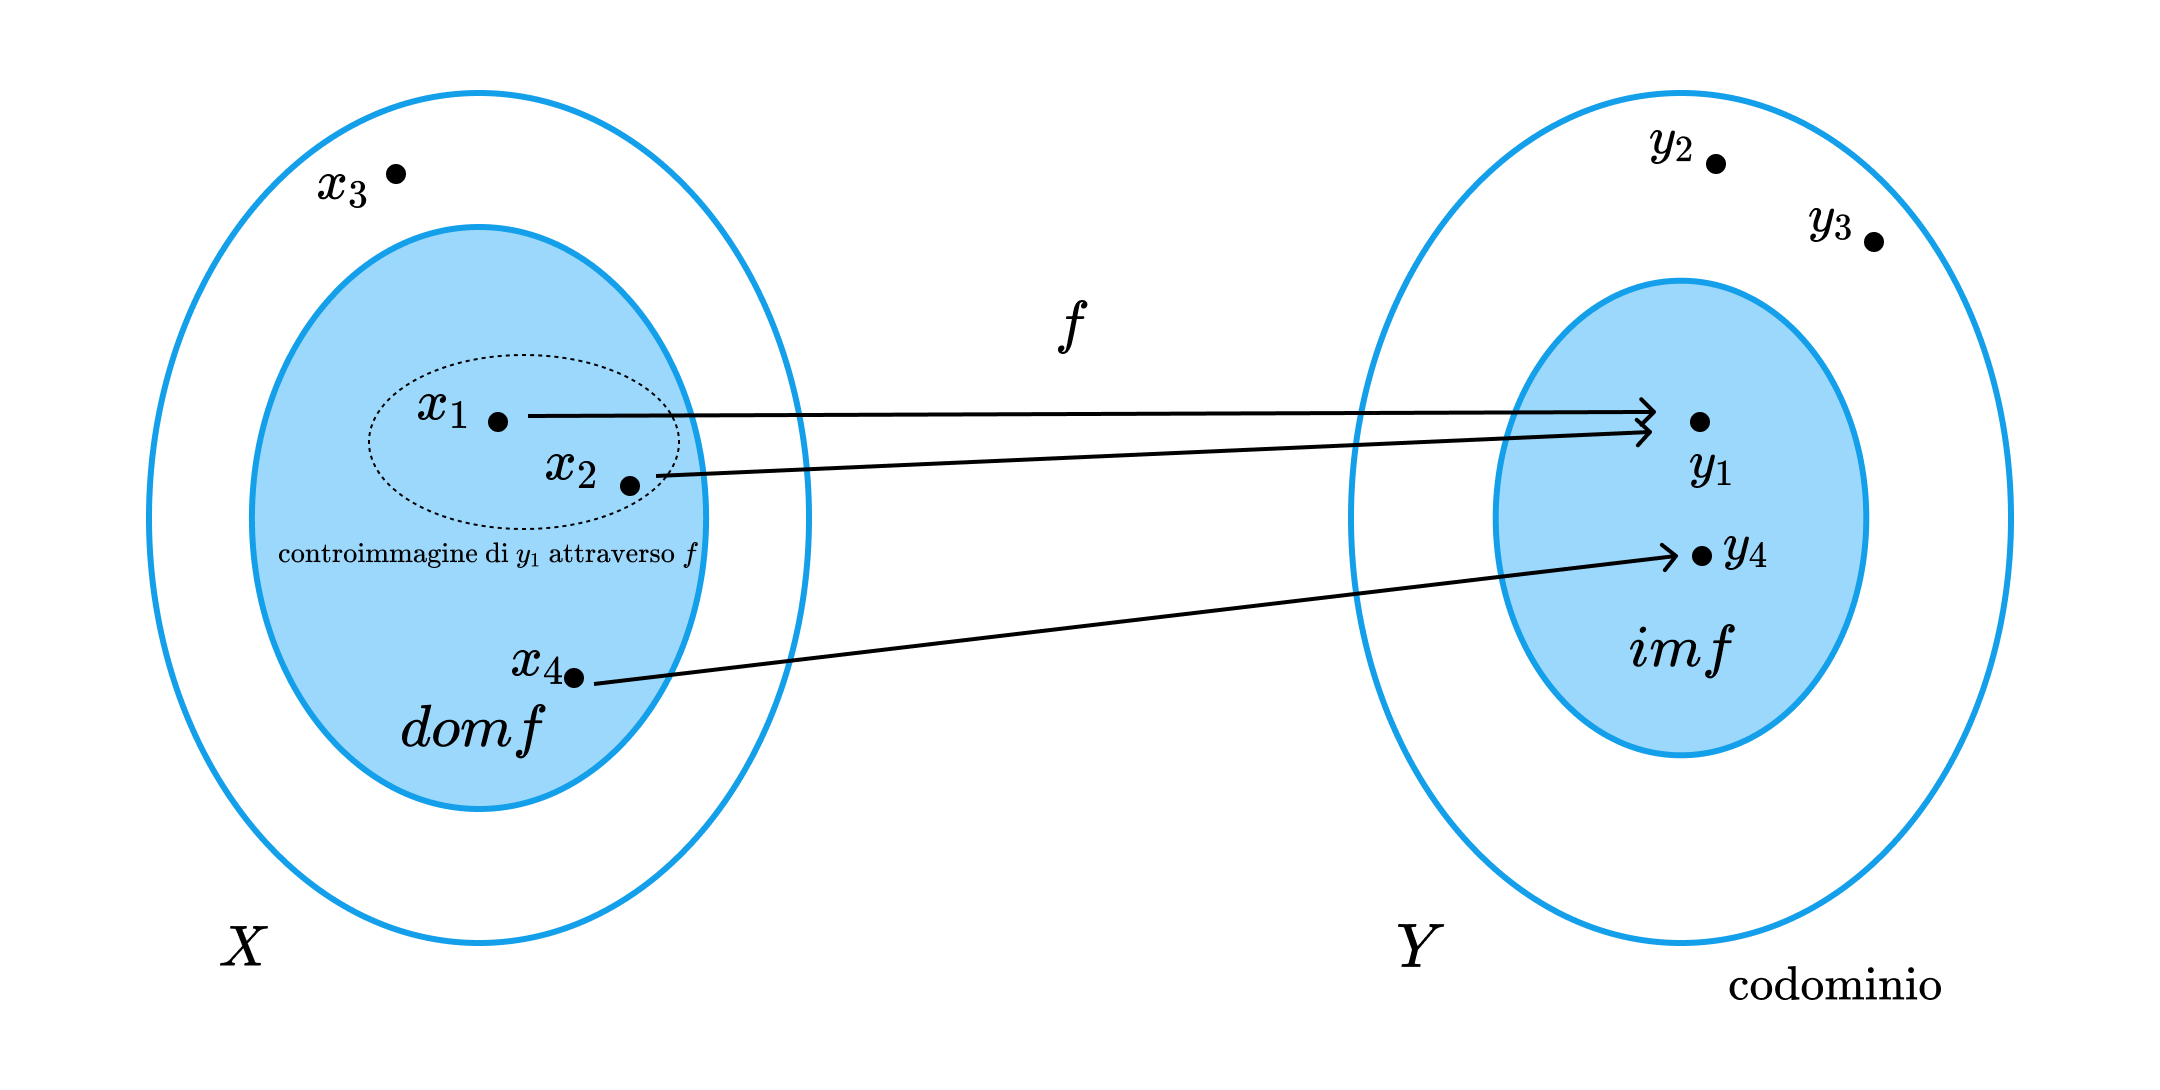
\includegraphics[width=0.8\textwidth]{source/00 funzione.png}
\end{center}

\begin{definition}
    \subsection{Dominio}
    Sia \( f: X \rightarrow Y \) una funzione. Il \textbf{dominio} di \( f \), indicato con \( \text{dom}(f) \), è l'insieme di tutti i valori di input per i quali la funzione \( f \) è definita. In termini formali,
    \[ \text{dom}(f) = X \]
    che è l'insieme da cui ogni \( x \) viene scelto per l'applicazione della funzione \( f \).
\end{definition}

\begin{definition}
    \subsection{Immagine}
    Sia \( f: X \rightarrow Y \) una funzione. L'\textbf{immagine} di \( f \), indicata con \( \text{im}(f) \), è l'insieme di tutti i valori che \( f \) può assumere come output. In termini formali,
    \[ \text{im}(f) = \{ f(x) \mid x \in X \} \]
    che è un sottoinsieme di \( Y \).
\end{definition}
\noindent\begin{minipage}{\textwidth}
    \begin{definition}
        \subsection{Codominio}
        Sia \( f: X \rightarrow Y \) una funzione. Il \textbf{codominio} di \( f \) è l'insieme \( Y \) stesso. Il codominio rappresenta tutti i possibili valori che \( f \) può teoricamente assumere come output, indipendentemente dal fatto che questi valori vengano effettivamente raggiunti o meno quando la funzione è applicata agli elementi di \( X \).

        Ad esempio, consideriamo la funzione \( f: \mathbb{R} \rightarrow \mathbb{R} \) definita da \( f(x) = x^2 \). Qui, il codominio è l'intero insieme dei numeri reali \( \mathbb{R} \), perché la funzione è definita in questo modo. Tuttavia, l'immagine di \( f \), cioè l'insieme dei valori che \( f \) effettivamente assume, è l'insieme dei numeri reali non negativi, poiché il quadrato di un numero reale non è mai negativo. Quindi, l'immagine è \( [0, \infty) \), un sottoinsieme del codominio \( \mathbb{R} \).
    \end{definition}
\end{minipage}

\begin{definition}
    \subsection{Controimmagine}
    Sia \( f: X \rightarrow Y \) una funzione e \( B \subseteq Y \) un sottoinsieme del codominio. La \textbf{controimmagine} (o pre-immagine) di \( B \) sotto \( f \), indicata con \( f^{-1}(B) \), è l'insieme di tutti gli elementi in \( X \) i cui valori sotto \( f \) appartengono a \( B \). In termini formali,
    \[ f^{-1}(B) = \{ x \in X \mid f(x) \in B \} \]
\end{definition}

\begin{example}
    \subsection{Esempi}
    Di seguito degli esempi di funzioni.
    \begin{enumerate}[label=\roman*., start=1]
        \item \noindent\begin{minipage}{\textwidth}
                  \(f : \mathbb{R} \rightarrow \mathbb{R}, f(x) = ax+ b\) (con a,b coefficienti reali), una \textbf{retta}
                  \begin{figure}[H]
                      \centering
                      \begin{tikzpicture}[scale = 1,
                              declare function={
                                      f(\x) = 2*\x - 2;
                                  }]
                          \begin{axis}
                              [
                                  xlabel={\( x \)},
                                  ylabel={\( f(x) \)},
                                  xmin=-10, xmax=10,
                                  ymin=-10, ymax=10,
                                  grid=both,
                                  axis lines=middle,
                                  axis line style=->,
                                  grid style={line width=.1pt, draw=gray!10},
                                  major grid style={line width=.2pt,draw=gray!50},
                                  minor tick num=3,
                                  enlargelimits={abs=0.5},
                                  xlabel style={at={(ticklabel* cs:1)}, anchor=north west},
                                  ylabel style={at={(ticklabel* cs:1)}, anchor=south west},
                                  samples=100,
                                  unbounded coords=jump,
                                  legend pos=south east
                              ]
                              \addplot[domain=-5:7, ultra thick, smooth, color=myblue]{f(x)};
                              \legend{\(f(x) = 2x - 2\)};
                          \end{axis}
                      \end{tikzpicture}
                      \caption{Grafico di \(f(x) = 2x - 2\)}
                  \end{figure}
              \end{minipage}
        \item \noindent\begin{minipage}{\textwidth}
                  \(f : \mathbb{R} \rightarrow \mathbb{R}, f(x) = x^2\), una \textbf{parabola}
                  \begin{figure}[H]
                      \centering
                      \begin{tikzpicture}[scale = 1,
                              declare function={
                                      f(\x) = \x^2;
                                  }]
                          \begin{axis}
                              [
                                  xlabel={\( x \)},
                                  ylabel={\( f(x) \)},
                                  xmin=-10, xmax=10,
                                  ymin=-10, ymax=10,
                                  grid=both,
                                  axis lines=middle,
                                  axis line style=->,
                                  grid style={line width=.1pt, draw=gray!10},
                                  major grid style={line width=.2pt,draw=gray!50},
                                  minor tick num=3,
                                  enlargelimits={abs=0.5},
                                  xlabel style={at={(ticklabel* cs:1)}, anchor=north west},
                                  ylabel style={at={(ticklabel* cs:1)}, anchor=south west},
                                  samples=100,
                                  unbounded coords=jump,
                                  legend pos=south east
                              ]
                              \addplot[domain=-5:5, ultra thick, smooth, color=myblue]{f(x)};
                              \legend{\(f(x) = x^2\)};
                          \end{axis}
                      \end{tikzpicture}
                      \caption{Grafico di \(f(x) = x^2\)}
                  \end{figure}
              \end{minipage}
        \item \noindent\begin{minipage}{\textwidth}
                  \(f : \mathbb{R}\setminus \{0\} \rightarrow \mathbb{R}, f(x) = \frac{1}{x}\), un'\textbf{iperbole} riferita agli asintoti
                  \begin{figure}[H]
                      \centering
                      \begin{tikzpicture}[scale = 1,
                              declare function={
                                      f(\x) = 1/\x;
                                  }]
                          \begin{axis}
                              [
                                  xlabel={\( x \)},
                                  ylabel={\( f(x) \)},
                                  xmin=-5, xmax=5,
                                  ymin=-5, ymax=5,
                                  grid=both,
                                  axis lines=middle,
                                  axis line style=->,
                                  grid style={line width=.1pt, draw=gray!10},
                                  major grid style={line width=.2pt,draw=gray!50},
                                  minor tick num=3,
                                  enlargelimits={abs=0.5},
                                  xlabel style={at={(ticklabel* cs:1)}, anchor=north west},
                                  ylabel style={at={(ticklabel* cs:1)}, anchor=south west},
                                  samples=100,
                                  unbounded coords=jump,
                                  legend pos=south east
                              ]
                              \addplot[domain=-6:-0.01, ultra thick, smooth, color=myblue]{f(x)};
                              \addplot[domain=0.01:6, ultra thick, smooth, color=myblue]{f(x)};
                              \legend{\(f(x) = \frac{1}{x}\)};
                          \end{axis}
                      \end{tikzpicture}
                      \caption{Grafico di \(f(x) = \frac{1}{x}\)}
                  \end{figure}
              \end{minipage}
        \item
              \noindent\begin{minipage}{\textwidth}
                  \(f : [0,3] \rightarrow \mathbb{R}\),
                  \(
                  f(x) =
                  \begin{cases}
                      3x    & \text{se } 0 \leq x \leq 1, \\
                      4 - x & \text{se } 1 < x \leq 2,    \\
                      x - 1 & \text{se } 2 < x \leq 3.
                  \end{cases}
                  \)
                  una funzione reale di variabile reale può essere \textbf{definita a tratti},
                  \begin{figure}[H]
                      \centering
                      \begin{tikzpicture}[scale = 1,
                              declare function={
                                      f(\x) = 3*\x;
                                      g(\x) = 4-\x;
                                      h(\x) = \x-1;
                                  }]
                          \begin{axis}
                              [
                                  xlabel={\( x \)},
                                  ylabel={\( f(x) \)},
                                  xmin=-4, xmax=4,
                                  ymin=-4, ymax=4,
                                  grid=both,
                                  axis lines=middle,
                                  axis line style=->,
                                  grid style={line width=.1pt, draw=gray!10},
                                  major grid style={line width=.2pt,draw=gray!50},
                                  minor tick num=3,
                                  enlargelimits={abs=0.5},
                                  xlabel style={at={(ticklabel* cs:1)}, anchor=north west},
                                  ylabel style={at={(ticklabel* cs:1)}, anchor=south west},
                                  samples=100,
                                  unbounded coords=jump,
                                  legend pos=south east
                              ]
                              \addplot[domain=0:1, ultra thick, smooth, color=myblue]{f(x)};
                              \addplot[domain=1:2, ultra thick, smooth, color=myblue]{g(x)};
                              \addplot[domain=2:3, ultra thick, smooth, color=myblue]{h(x)};
                              \filldraw [white] (2 , 1) circle (1.5pt);
                              \draw [myblue] (2 , 1) circle (1.5pt);
                              \filldraw [myblue] (2 , 2) circle (1.5pt);
                          \end{axis}
                      \end{tikzpicture}
                      \caption{Grafico di una funzione definita a tratti}
                  \end{figure}
              \end{minipage}
        \item \noindent\begin{minipage}{\textwidth}
                  \(f : \mathbb{R} \rightarrow \mathbb{R}, \space f(x) = |x| \)
                  \(
                  f(x) = |x| =
                  \begin{cases}
                      x  & \text{se } x \geq 0, \\
                      -x & \text{se } x < 0.
                  \end{cases}
                  \)
                  la funzione \textbf{Valore Assoluto}
                  \begin{figure}[H]
                      \centering
                      \begin{tikzpicture}[scale = 1,
                              declare function={
                                      f(\x) = -\x;
                                      g(\x) = \x;
                                  }]
                          \begin{axis}
                              [
                                  xlabel={\( x \)},
                                  ylabel={\( f(x) \)},
                                  xmin=-4, xmax=4,
                                  ymin=-4, ymax=4,
                                  grid=both,
                                  axis lines=middle,
                                  axis line style=->,
                                  grid style={line width=.1pt, draw=gray!10},
                                  major grid style={line width=.2pt,draw=gray!50},
                                  minor tick num=3,
                                  enlargelimits={abs=0.5},
                                  xlabel style={at={(ticklabel* cs:1)}, anchor=north west},
                                  ylabel style={at={(ticklabel* cs:1)}, anchor=south west},
                                  samples=100,
                                  unbounded coords=jump,
                                  legend pos=south east
                              ]
                              \addplot[domain=-5:0, ultra thick, smooth, color=myblue]{f(x)};
                              \addplot[domain=0:5, ultra thick, smooth, color=myblue]{g(x)};
                              \legend{\(f(x) = |x|\)};
                          \end{axis}
                      \end{tikzpicture}
                      \caption{Grafico di \(f(x) = |x|\)}
                  \end{figure}
              \end{minipage}
        \item
              \noindent\begin{minipage}{\textwidth}
                  \(f : \mathbb{R} \rightarrow \mathbb{Z}, \space f(x) = sign(x) \)
                  \(
                  f(x) = sign(x) =
                  \begin{cases}
                      +1 & \text{se } x > 0, \\
                      0  & \text{se }  x = 0 \\
                      -1 & \text{se} x < 0.
                  \end{cases}
                  \)
                  la funzione \textbf{Segno}
                  \begin{figure}[H]
                      \centering
                      \begin{tikzpicture}[scale = 1,
                              declare function={
                                      f(\x) = -1;
                                      g(\x) = 1;
                                  }]
                          \begin{axis}
                              [
                                  xlabel={\( x \)},
                                  ylabel={\( f(x) \)},
                                  xmin=-4, xmax=4,
                                  ymin=-4, ymax=4,
                                  grid=both,
                                  axis lines=middle,
                                  axis line style=->,
                                  grid style={line width=.1pt, draw=gray!10},
                                  major grid style={line width=.2pt,draw=gray!50},
                                  minor tick num=3,
                                  enlargelimits={abs=0.5},
                                  xlabel style={at={(ticklabel* cs:1)}, anchor=north west},
                                  ylabel style={at={(ticklabel* cs:1)}, anchor=south west},
                                  samples=100,
                                  unbounded coords=jump,
                                  legend pos=south east
                              ]
                              \addplot[domain=-5:0, ultra thick, smooth, color=myblue]{f(x)};
                              \addplot[domain=0:5, ultra thick, smooth, color=myblue]{g(x)};
                              \filldraw [myblue] (0 , 0) circle (1.5pt);
                              \filldraw [white] (0 , -1) circle (1.5pt);
                              \filldraw [white] (0 , 1) circle (1.5pt);
                              \draw [myblue] (0 , -1) circle (1.5pt);
                              \draw [myblue] (0 , 1) circle (1.5pt);
                              \legend{\(f(x) = sign(x)\)};
                          \end{axis}
                      \end{tikzpicture}
                      \caption{Grafico di \(f(x) = sign(x)\)}
                  \end{figure}
              \end{minipage}
        \item
              \noindent\begin{minipage}{\textwidth}
                  \(f : \mathbb{R} \rightarrow \mathbb{Z}, \space f(x) = [x] =\)  il più grande intero relativo \(\leq x\),  la funzione \textbf{Parte intera}
                  \begin{figure}[H]
                      \centering
                      \begin{tikzpicture}[scale = 1,
                              declare function={
                                      f(\x) = -2;
                                      g(\x) = -1;
                                      h(\x) = 0;
                                      i(\x) = 1;
                                      j(\x) = 2;
                                  }]
                          \begin{axis}
                              [
                                  xlabel={\( x \)},
                                  ylabel={\( f(x) \)},
                                  xmin=-2, xmax=2,
                                  ymin=-2, ymax=2,
                                  grid=both,
                                  axis lines=middle,
                                  axis line style=->,
                                  grid style={line width=.1pt, draw=gray!10},
                                  major grid style={line width=.2pt,draw=gray!50},
                                  minor tick num=3,
                                  enlargelimits={abs=0.5},
                                  xlabel style={at={(ticklabel* cs:1)}, anchor=north west},
                                  ylabel style={at={(ticklabel* cs:1)}, anchor=south west},
                                  samples=100,
                                  unbounded coords=jump,
                                  legend pos=south east
                              ]
                              \addplot[domain=-2:-1, ultra thick, smooth, color=myblue]{f(x)};
                              \addplot[domain=-1:0, ultra thick, smooth, color=myblue]{g(x)};
                              \addplot[domain=0:1, ultra thick, smooth, color=myblue]{h(x)};
                              \addplot[domain=1:2, ultra thick, smooth, color=myblue]{i(x)};
                              \addplot[domain=2:3, ultra thick, smooth, color=myblue]{j(x)};
                              \filldraw [white] (-2 , -2) circle (1.5pt);
                              \filldraw [white] (-1, -1) circle (1.5pt);
                              \filldraw [white] (0 , 0) circle (1.5pt);
                              \filldraw [white] (1 , 1) circle (1.5pt);
                              \filldraw [white] (2 , 2) circle (1.5pt);
                              \draw [myblue] (-2 , -2) circle (1.5pt);
                              \draw [myblue] (-1 , -1) circle (1.5pt);
                              \draw [myblue] (0 , 0) circle (1.5pt);
                              \draw [myblue] (1 , 1) circle (1.5pt);
                              \draw [myblue] (2 , 2) circle (1.5pt);
                              \filldraw [myblue] (-1 , -2) circle (1.5pt);
                              \filldraw [myblue] (0 , -1) circle (1.5pt);
                              \filldraw [myblue] (1 , 0) circle (1.5pt);
                              \filldraw [myblue] (2 , 1) circle (1.5pt);
                              \legend{\(f(x) = [x]\)};
                          \end{axis}
                      \end{tikzpicture}
                      \caption{Grafico di \(f(x) = [x]\)}
                  \end{figure}
              \end{minipage}
    \end{enumerate}
\end{example}
\newpage
\section{Funzioni iniettive, suriettive, biiettive}
Le tre proprietà che definiremo hanno un immediato riscontro grafico
nel caso di funzioni \(f\) reali di variabile reale. Precisamente, considerando il
grafico di \(f\) nel piano e le sue intersezioni con la famiglia di rette orizzontali,
la funzione risulta
\begin{enumerate}
    \item \textbf{iniettiva} se lo interseca al massimo in un punto,
    \item \textbf{suriettiva} su \(\mathbb{R}\) se ogni retta interseca il grafico in almeno un punto,
    \item \textbf{biiettiva} da \(\mathbb{R} \rightarrow \mathbb{R}\) se lo interseca esattamente in uno e un solo punto
\end{enumerate}
\noindent\begin{minipage}{\textwidth}
    \begin{definition}
        \subsection{Funzione iniettiva}
        Sia \(f:A \rightarrow B\). La funzione \(f\) è detta iniettiva se, per ogni coppia di elementi \(a_1, a_2 \in A\), \(a_1 \neq a_2\) \(\Rightarrow\) \(f(a_1) \neq f(a_2)\).
    \end{definition}
    \begin{figure}[H]
        \centering
        \begin{tikzpicture}
            \begin{axis}[
                    xlabel={\( x \)},
                    ylabel={\( f(x) \)},
                    xmin=-2, xmax=2,
                    ymin=-2, ymax=2,
                    grid=both,
                    axis lines=middle,
                    axis line style=->,
                    grid style={line width=.1pt, draw=gray!10},
                    major grid style={line width=.2pt,draw=gray!50},
                    minor tick num=5,
                    enlargelimits={abs=0.5},
                    ticklabel style={font=\small},
                    xlabel style={at={(ticklabel* cs:1)}, anchor=north west},
                    ylabel style={at={(ticklabel* cs:1)}, anchor=south west},
                    legend pos=south east
                ]
                \addplot[domain=-3:3, ultra thick, smooth, color=myblue] {x};
                \legend{Iniettiva}
            \end{axis}
        \end{tikzpicture}
        \begin{tikzpicture}
            \begin{axis}[
                    xlabel={\( x \)},
                    ylabel={\( f(x) \)},
                    xmin=-2, xmax=2,
                    ymin=-2, ymax=2,
                    grid=both,
                    axis lines=middle,
                    axis line style=->,
                    grid style={line width=.1pt, draw=gray!10},
                    major grid style={line width=.2pt,draw=gray!50},
                    minor tick num=5,
                    enlargelimits={abs=0.5},
                    ticklabel style={font=\small},
                    xlabel style={at={(ticklabel* cs:1)}, anchor=north west},
                    ylabel style={at={(ticklabel* cs:1)}, anchor=south west},
                    legend pos=south east
                ]
                \addplot[domain=-2:2, ultra thick, smooth, color=myblue] {x^2};
                \coordinate (A) at (axis cs:-1,1);
                \coordinate (B) at (axis cs:1,1);
                \coordinate (C) at (axis cs:-1,0);
                \coordinate (D) at (axis cs:1,0);
                \node at (A)[left] {$f(a_1)$};
                \node at (B)[right] {$f(a_2)$};
                \node at (C)[below left] {$a_1$};
                \node at (D)[below right] {$a_2$};
                \draw [dashed,thick](A) -- (B);
                \draw [dashed,thick](A) -- (C);
                \draw [dashed,thick](B) -- (D);
                \legend{Non iniettiva};
            \end{axis}
        \end{tikzpicture}
        \caption{Confronto tra una \(f(x)=x\) iniettiva, e \(f(x)=x^2\) non iniettiva}
    \end{figure}
\end{minipage}
\noindent\begin{minipage}{\textwidth}
    \begin{definition}
        \subsection{Funzione suriettiva}
        Sia \(f:A \rightarrow B\), se
        \[\ \forall\ b \in B, \exists\ f(a)=b\]
        allora f è suriettiva.
    \end{definition}
    \begin{figure}[H]
        \centering
        \begin{tikzpicture}
            \begin{axis}[
                    xlabel={\( x \)},
                    ylabel={\( f(x) \)},
                    xmin=-2, xmax=2,
                    ymin=-2, ymax=2,
                    grid=both,
                    axis lines=middle,
                    axis line style=->,
                    grid style={line width=.1pt, draw=gray!10},
                    major grid style={line width=.2pt,draw=gray!50},
                    minor tick num=5,
                    enlargelimits={abs=0.5},
                    ticklabel style={font=\small},
                    xlabel style={at={(ticklabel* cs:1)}, anchor=north west},
                    ylabel style={at={(ticklabel* cs:1)}, anchor=south west},
                    legend pos=south east
                ]
                \addplot[domain=-3:3, ultra thick, smooth, color=myblue] {x};
                \legend{Suriettiva}
            \end{axis}
        \end{tikzpicture}
        \begin{tikzpicture}
            \begin{axis}[
                    xlabel={\( x \)},
                    ylabel={\( f(x) \)},
                    xmin=-2, xmax=2,
                    ymin=-2, ymax=2,
                    grid=both,
                    axis lines=middle,
                    axis line style=->,
                    grid style={line width=.1pt, draw=gray!10},
                    major grid style={line width=.2pt,draw=gray!50},
                    minor tick num=5,
                    enlargelimits={abs=0.5},
                    ticklabel style={font=\small},
                    xlabel style={at={(ticklabel* cs:1)}, anchor=north west},
                    ylabel style={at={(ticklabel* cs:1)}, anchor=south west},
                    legend pos=south east
                ]
                \addplot[domain=-2:2, ultra thick, smooth, color=myblue] {x^2};
                \coordinate (A) at (axis cs:-3,0);
                \coordinate (B) at (axis cs:+3,0);
                \coordinate (C) at (axis cs:3,-3);
                \coordinate (D) at (axis cs:-3,-3);
                \fill[myblue, opacity=0.5] (A) -- (B) -- (C) -- (D) -- cycle;
                \legend{Non suriettiva};
            \end{axis}
        \end{tikzpicture}
        \caption{Confronto tra una \(f(x)=x\) suriettiva, e \(f(x)=x^2\) non suriettiva}
    \end{figure}
\end{minipage}
\begin{definition}
    \subsection{Funzione biunivoca}
    Sia \(f:A \rightarrow B\), se \(f\) è sia iniettiva che suriettiva, allora f è biiettiva(o biunivoca).
\end{definition}
\section{Funzione inversa}

La nozione di funzione inversa è centrale nell'analisi matematica e nelle sue applicazioni. Data una funzione \( f: A \rightarrow B \), l'inversa di \( f \), denotata come \( f^{-1} \), è una funzione da \( B \) a \( A \) tale che per ogni \( y \) nell'immagine di \( f \), \( f^{-1}(y) \) restituisce l'unico \( x \) in \( A \) per cui \( f(x) = y \).

\subsection{Condizioni per l'Invertibilità}
Una funzione deve essere iniettiva per avere un'inversa. L'iniettività garantisce che ogni elemento dell'immagine di \( f \) è associato a un unico elemento del dominio. Questa unicità è essenziale per definire \( f^{-1} \).

\subsection{Calcolo della Funzione Inversa}
Calcolare l'inversa di una funzione può essere un processo complesso. Per le funzioni algebriche, il metodo standard consiste nel risolvere l'equazione \( y = f(x) \) rispetto a \( x \). Questo approccio funziona bene per molte funzioni semplici. Tuttavia, esistono funzioni iniettive le cui inverse non possono essere espresse in forma chiusa. Una forma chiusa è un'espressione matematica finita che utilizza un numero finito di operazioni algebriche standard e funzioni elementari. Alcune funzioni iniettive, pur essendo teoricamente invertibili, non hanno un'espressione inversa semplice e diretta in termini di funzioni e operazioni elementari.


\subsection{Grafico della Funzione Inversa}
Il grafico di \( f^{-1} \) può essere ottenuto dal grafico di \( f \) scambiando gli assi \( x \) e \( y \). Questo scambio è equivalente a riflettere il grafico di \( f \) rispetto alla linea \( y = x \).
\begin{example}
    Prendo \[f :\ \mathbb{R} \rightarrow \mathbb{R},\ f(x) = x^2\]
    non è iniettiva.\\
    Prendo una \textbf{restrizione} \(A\) del dominio di \(f\), \(A=[0,+\infty)\) per renderla iniettiva.
    \[f|_{A}: [0,+\infty) \rightarrow \mathbb{R}, f(x) = x^2\]
    tale funzione è iniettiva e dunque invertibile e l'inversa è
    \[f|_{A}: [0,+\infty) \rightarrow \mathbb{R}, x = f^{-1}(y) = +\sqrt{y}\]
    Si preferisce effettuare il cambio di notazioni
    \[f|_{A}: [0,+\infty) \rightarrow \mathbb{R}, y = f^{-1}(x) = +\sqrt{x}\]
    \begin{figure}[H]
        \centering
        \begin{tikzpicture}
            \begin{axis}[
                    xlabel={\( x \)},
                    ylabel={\( f(x) \)},
                    xmin=0, xmax=2,
                    ymin=0, ymax=2,
                    grid=both,
                    axis lines=middle,
                    axis line style=->,
                    grid style={line width=.1pt, draw=gray!10},
                    major grid style={line width=.2pt,draw=gray!50},
                    minor tick num=5,
                    enlargelimits={abs=0.5},
                    xlabel style={at={(ticklabel* cs:1)}, anchor=north west},
                    ylabel style={at={(ticklabel* cs:1)}, anchor=south west},
                    samples=100,
                    unbounded coords=jump, % Gestisce i punti non definiti
                    legend pos=south east
                ]
                \addplot[domain=0:2, ultra thick, smooth, color=gray] {x^2};
                \addplot[domain=-0.5:3, thick, dashed, color=black] {x};
                \addplot[domain=0:3, ultra thick, smooth, color=myblue] {sqrt(x)};
                \legend{$y=x^2$, $y=x$, $y=+\sqrt{x}$};
            \end{axis}
        \end{tikzpicture}
    \end{figure}
\end{example}
\subsection{Ambiguità nella notazione e nel calcolo}
\begin{itemize}
    \item La notazione \( f^{-1} \) per la funzione inversa può portare a confusione, in particolare per chi si avvicina per la prima volta allo studio delle funzioni inverse. A differenza dell'inverso moltiplicativo, dove \( a^{-1} \) rappresenta l'elemento che, moltiplicato per \( a \), dà come risultato l'elemento neutro della moltiplicazione (tipicamente 1), la notazione \( f^{-1} \) non implica un'operazione aritmetica di inversione. Piuttosto, indica una funzione tale che, per ogni elemento \( y \) nell'immagine di \( f \), \( f^{-1}(y) \) restituisce l'elemento \( x \) del dominio di \( f \) per cui \( f(x) = y \).
    \item Un'altra fonte di ambiguità è il calcolo effettivo dell'espressione analitica di \( f^{-1} \). Per alcune funzioni, trovare la forma chiusa della funzione inversa è relativamente semplice e diretto, come nel caso delle funzioni lineari. Tuttavia, per altre funzioni, in particolare quelle non lineari o quelle che coinvolgono operazioni complesse, determinare \( f^{-1} \) in una forma esplicita può essere estremamente difficile, se non impossibile. Questo è dovuto al fatto che l'operazione di "invertire" una funzione non segue un processo standard e può richiedere metodi matematici avanzati o, in alcuni casi, può non avere una soluzione in termini di funzioni elementari.
    \item Inoltre, quando si riesce a trovare una formula per \( f^{-1} \), \textbf{spesso si effettua un cambio di variabili} per comodità. Inizialmente, se abbiamo \( x = f^{-1}(y) \), si può preferire riscrivere questa relazione come \( y = f^{-1}(x) \), scambiando semplicemente i simboli delle variabili. Questo non solo aiuta a mantenere una consistenza nella notazione, ma facilita anche il confronto e la rappresentazione grafica di \( f \) e \( f^{-1} \) sullo stesso sistema di coordinate. Un esempio di questo può essere visto nella transizione da una rappresentazione grafica a un'altra, come illustrato nella Figura 2.7 del testo, dove si passa da un grafico della funzione originale \( f \) a quello della sua inversa \( f^{-1} \).

\end{itemize}
\subsection{Esempi e Applicazioni}
\begin{itemize}
    \item \textbf{Funzione Logaritmica:} L'inversa della funzione esponenziale \( e^x \) è il logaritmo naturale \( \ln(x) \).
    \item \textbf{Funzioni Trigonometriche:} Le funzioni trigonometriche hanno inverse note come funzioni arcotrigonometriche, ma queste sono definite solo su intervalli specifici per mantenere l'iniettività.
\end{itemize}

\section{Funzioni monot\'one}
\begin{definition}
    \subsection{Funzione Monotona Crescente}
    Una funzione \( f \) si dice \textbf{monotona crescente} su un intervallo \( I \) se, per qualsiasi coppia di elementi \( x_1 \) e \( x_2 \) in \( I \) tali che \( x_1 < x_2 \), risulta sempre che \( f(x_1) \leq f(x_2) \). In forma simbolica, questo si esprime come:
    \[ \forall x_1, x_2 \in I, x_1 < x_2 \Rightarrow f(x_1) \leq f(x_2). \]

    Inoltre, la funzione \( f \) si dice \textbf{monotona strettamente crescente} su \( I \) se, per ogni coppia di elementi \( x_1 \) e \( x_2 \) in \( I \) con \( x_1 < x_2 \), si ha che \( f(x_1) < f(x_2) \). Questa condizione si può scrivere come:
    \[ \forall x_1, x_2 \in I, x_1 < x_2 \Rightarrow f(x_1) < f(x_2). \]
\end{definition}
\begin{figure}[H]
    \centering
    \begin{tikzpicture}
        \begin{axis}[
                xlabel={\( x \)},
                ylabel={\( y \)},
                xmin=0, xmax=2,
                ymin=0, ymax=2,
                grid=both,
                axis lines=middle,
                axis line style=->,
                grid style={line width=.1pt, draw=gray!10},
                major grid style={line width=.2pt,draw=gray!50},
                minor tick num=5,
                enlargelimits={abs=0.5},
                ticklabel style={font=\small},
                xlabel style={at={(ticklabel* cs:1)}, anchor=north west},
                ylabel style={at={(ticklabel* cs:1)}, anchor=south west},
                legend pos=south east
            ]
            \coordinate (A) at (axis cs:0.5,0.25);
            \coordinate (B) at (axis cs:1,1);
            \coordinate (Ay) at (axis cs:0,0.25);
            \coordinate (Ax) at (axis cs:0.5,0);
            \coordinate (By) at (axis cs:0,1);
            \coordinate (Bx) at (axis cs:1,0);
            \draw [dashed,thick](A) -- (Ay);
            \draw [dashed,thick](A) -- (Ax);
            \draw [dashed,thick](B) -- (Bx);
            \draw [dashed,thick](B) -- (By);
            \addplot[myblue, ultra thick, smooth, domain=0:2] {x^2};
            \filldraw [myblue] (A) circle (1.5pt);
            \filldraw [myblue] (B) circle (1.5pt);
            \legend{$y=x^2$};
        \end{axis}
    \end{tikzpicture}
    \caption{Funzione strettamente crescente su un intervallo I}
\end{figure}
\begin{proposition}
    Se \(f\) è strettamente monotona sul suo dominio, allora \(f\) è iniettiva.
\end{proposition}

\section{Funzioni composte}
\begin{definition}
    \subsection{Funzione Composta}
    Siano \( X \), \( Y \) e \( Z \) tre insiemi distinti. Sia \( f \) una funzione definita da \( X \) a \( Y \), e sia \( g \) una funzione definita da \( Y \) a \( Z \). Possiamo costruire una nuova funzione \( h \) definita da \( X \) a \( Z \) come la composizione di \( f \) e \( g \). Questa nuova funzione \( h \) è definita ponendo per ogni \( x \in X \):
    \[ h(x) = g(f(x)) \]
    \[h = g \circ f\]
\end{definition}

\section{Trasformazioni geometriche}
\begin{definition}
    \subsection{Traslazione di funzione mediante vettore(a,b)}
    Di seguito le traslazioni dato un vettore
    \( \vec{v} = (a,b)\text{, con }a>0, b>0 \)
    Ricordo che la traslazione di un punto di ottiene mediante
    \[T=\begin{cases}
            x_T=x+a \\
            y_T=y+b
        \end{cases}\]
    Mentre la traslazione di una funzione di ottiene mediante
    \[T^{-1}=\begin{cases}
            x_T=x-a \\
            y_T=y-b
        \end{cases}\]
\end{definition}
\subsubsection{Traslazione di vettore parallelo all’asse y (a=0,b=2).}
\[T^{-1}=\begin{cases}
        x_T=x-0 \\
        y_T=y-2
    \end{cases}\]
\begin{align*}
     & y_T = sin( x_T )     \\
     & y - 2 = sin( x - 0 ) \\
     & y = sin( x ) + 2
\end{align*}
\begin{figure}[H]
    \begin{center}
        \begin{animateinline}[controls,loop]{60}
            \multiframe{10}{rAlpha=0+0.2}{% Incrementa alpha
                \begin{tikzpicture}
                    \begin{axis}[
                            title={Animazione},
                            xlabel={\( x \)},
                            ylabel={\( y \)},
                            xmin=-5, xmax=5,
                            ymin=-5, ymax=5,
                            grid=both,
                            axis lines=middle,
                            axis line style=->,
                            grid style={line width=.1pt, draw=gray!10},
                            major grid style={line width=.2pt,draw=gray!50},
                            minor tick num=5,
                            enlargelimits={abs=0.5},
                            ticklabel style={font=\small},
                            xlabel style={at={(ticklabel* cs:1)}, anchor=north west},
                            ylabel style={at={(ticklabel* cs:1)}, anchor=south west},
                            legend pos=south east
                        ]
                        \addplot[domain=-5:5, ultra thick, smooth, color=myblue] {sin(deg(x))+\rAlpha};
                        \draw[-latex, ultra thick, color=red] (0,0) -- (0,+\rAlpha);
                        \node[above] at (0,+\rAlpha) {$\vec{v}=(0,\rAlpha)$};
                        \legend{{$\sin(x) + \rAlpha$}}
                    \end{axis}
                \end{tikzpicture}
            }
        \end{animateinline}
        \begin{tikzpicture}
            \begin{axis}[
                    xlabel={\( x \)},
                    ylabel={\( y \)},
                    xmin=-5, xmax=5,
                    ymin=-5, ymax=5,
                    grid=both,
                    axis lines=middle,
                    axis line style=->,
                    grid style={line width=.1pt, draw=gray!10},
                    major grid style={line width=.2pt,draw=gray!50},
                    minor tick num=5,
                    enlargelimits={abs=0.5},
                    ticklabel style={font=\small},
                    xlabel style={at={(ticklabel* cs:1)}, anchor=north west},
                    ylabel style={at={(ticklabel* cs:1)}, anchor=south west},
                    legend pos=south east
                ]
                \addplot[domain=-5:5, ultra thick, smooth, color=black] {sin(deg(x))};
                \addplot[domain=-5:5, ultra thick, smooth, color=myblue] {sin(deg(x))+2};
                \draw[-latex, ultra thick, color=red] (0,0) -- (0,2);
                \node[above] at (0,2) {$\vec{v}=(0,2)$};
                \legend{{$\sin(x)$}, {$\sin(x) + 2$}}
            \end{axis}
        \end{tikzpicture}
    \end{center}
    \caption{Traslazione di vettore parallelo all’asse y}
\end{figure}

\subsubsection{Traslazione di vettore parallelo all’asse x.\textcolor{myblue}{!!!} (a=2,b=0).}
\[T^{-1}=\begin{cases}
        x_T=x-2 \\
        y_T=y-0
    \end{cases}\]
\begin{align*}
     & y_T = sin( x_T )     \\
     & y - 0 = sin( x - 2 ) \\
     & y = sin( x - 2)
\end{align*}
\begin{figure}[H]
    \centering
    \begin{animateinline}[controls,loop]{60}
        \multiframe{10}{rAlpha=0+0.2}{% Incrementa alpha
            \begin{tikzpicture}
                \begin{axis}[
                        title=Animazione,
                        xlabel={\( x \)},
                        ylabel={\( y \)},
                        xmin=-5, xmax=5,
                        ymin=-5, ymax=5,
                        grid=both,
                        axis lines=middle,
                        axis line style=->,
                        grid style={line width=.1pt, draw=gray!10},
                        major grid style={line width=.2pt,draw=gray!50},
                        minor tick num=5,
                        enlargelimits={abs=0.5},
                        ticklabel style={font=\small},
                        xlabel style={at={(ticklabel* cs:1)}, anchor=north west},
                        ylabel style={at={(ticklabel* cs:1)}, anchor=south west},
                        legend pos=south east
                    ]
                    \addplot[domain=-5:5, ultra thick, smooth, color=myblue] {sin(deg(x-\rAlpha))};
                    \draw[-latex, ultra thick, color=red] (0,0) -- (\rAlpha,0);
                    \node[above] at (\rAlpha,0) {$\vec{v}=(\rAlpha,0)$};
                    \legend{{$\sin(x - \rAlpha)$}}
                \end{axis}
            \end{tikzpicture}
        }
    \end{animateinline}
    \begin{tikzpicture}
        \begin{axis}[
                xlabel={\( x \)},
                ylabel={\( y \)},
                xmin=-5, xmax=5,
                ymin=-5, ymax=5,
                grid=both,
                axis lines=middle,
                axis line style=->,
                grid style={line width=.1pt, draw=gray!10},
                major grid style={line width=.2pt,draw=gray!50},
                minor tick num=5,
                enlargelimits={abs=0.5},
                ticklabel style={font=\small},
                xlabel style={at={(ticklabel* cs:1)}, anchor=north west},
                ylabel style={at={(ticklabel* cs:1)}, anchor=south west},
                legend pos=south east
            ]
            \addplot[domain=-5:5, ultra thick, smooth, color=black] {sin(deg(x))};
            \addplot[domain=-5:5, ultra thick, smooth, color=myblue] {sin(deg(x-2))};
            \draw[-latex, ultra thick, color=red] (0,0) -- (2,0);
            \node[above] at (2,0) {$\vec{v}=(2,0)$};
            \legend{{$\sin(x)$}, {$\sin(x-2)$}}
        \end{axis}
    \end{tikzpicture}
    \caption{Traslazione di vettore parallelo all'asse x}
\end{figure}

\subsubsection{Traslazione di vettore qualsiasi.(a=2,b=2).}
\[T^{-1}=\begin{cases}
        x_T=x-2 \\
        y_T=y-2
    \end{cases}\]
\begin{align*}
     & y_T = sin( x_T )     \\
     & y - 2 = sin( x - 2 ) \\
     & y = sin( x - 2) +2
\end{align*}

\begin{figure}[H]
    \centering
    \begin{animateinline}[controls,loop]{60}
        \multiframe{10}{rab=0+0.2}{
            \begin{tikzpicture}
                \begin{axis}[
                        title=Animazione,
                        xlabel={\( x \)},
                        ylabel={\( y \)},
                        xmin=-5, xmax=5,
                        ymin=-5, ymax=5,
                        grid=both,
                        axis lines=middle,
                        axis line style=->,
                        grid style={line width=.1pt, draw=gray!10},
                        major grid style={line width=.2pt,draw=gray!50},
                        minor tick num=5,
                        enlargelimits={abs=0.5},
                        ticklabel style={font=\small},
                        xlabel style={at={(ticklabel* cs:1)}, anchor=north west},
                        ylabel style={at={(ticklabel* cs:1)}, anchor=south west},
                        legend pos=south east
                    ]
                    \addplot[domain=-5:5, ultra thick, smooth, color=myblue] {sin(deg(x-\rab))+\rab};
                    \draw[-latex, ultra thick, color=red] (0,0) -- (\rab, \rab);
                    \node[above] at (\rab, \rab) {$\vec{v}=(\rab,\rab)$};
                    \legend{{$\sin(x - \rab) + \rab$}, {$\sin(x - 2) + 2$}}
                \end{axis}
            \end{tikzpicture}
        }
    \end{animateinline}
    \begin{tikzpicture}
        \begin{axis}[
                xlabel={\( x \)},
                ylabel={\( y \)},
                xmin=-5, xmax=5,
                ymin=-5, ymax=5,
                grid=both,
                axis lines=middle,
                axis line style=->,
                grid style={line width=.1pt, draw=gray!10},
                major grid style={line width=.2pt,draw=gray!50},
                minor tick num=5,
                enlargelimits={abs=0.5},
                ticklabel style={font=\small},
                xlabel style={at={(ticklabel* cs:1)}, anchor=north west},
                ylabel style={at={(ticklabel* cs:1)}, anchor=south west},
                legend pos=south east
            ]
            \addplot[domain=-5:5, ultra thick, smooth, color=black] {sin(deg(x))};
            \addplot[domain=-5:5, ultra thick, smooth, color=myblue] {sin(deg(x-2))+2};
            \draw[-latex, ultra thick, color=red] (0,0) -- (2,2);
            \node[above] at (2,2) {$\vec{v}=(2,2)$};
            \legend{{$\sin(x)$},{$\sin(x-2)+2$}}
        \end{axis}
    \end{tikzpicture}
    \caption{Grafici di traslazioni di funzioni di un vettore qualsiasi}
\end{figure}
\begin{definition}
    \subsection{Cambiamento di scala}
    \begin{align*}
         & y=f(xc) = \begin{cases}
                         \text{contrazione orizzontale, se } c > 1                                             \\
                         \text{dilatazione orizzontale, se } 0 < c < 1                                         \\
                         \text{dilatazione o contrazione orizzontale + riflessione rispetto asse y, se } c < 0 \\
                     \end{cases} \\
         & y=f(x)c = \begin{cases}
                         \text{allungata verticalmente, se } c > 1                 \\
                         \text{compressa verticalmente, se } 0 < c < 1             \\
                         \text{scalatura + riflessione rispetto asse x, se } c < 0 \\
                     \end{cases}
    \end{align*}
\end{definition}
\subsubsection{Dilatazione/Contrazione orizzontale}
\begin{figure}[H]
    \centering
    \begin{animateinline}[controls,loop]{72}
        \multiframe{12}{rCoef=-1+0.4}{% Incrementa alpha
            \begin{tikzpicture}
                \begin{axis}[
                        title=Animazione,
                        xlabel={\( x \)},
                        ylabel={\( y \)},
                        xmin=-5, xmax=5,
                        ymin=-5, ymax=5,
                        grid=both,
                        axis lines=middle,
                        axis line style=->,
                        grid style={line width=.1pt, draw=gray!10},
                        major grid style={line width=.2pt,draw=gray!50},
                        minor tick num=5,
                        enlargelimits={abs=0.5},
                        ticklabel style={font=\small},
                        xlabel style={at={(ticklabel* cs:1)}, anchor=north west},
                        ylabel style={at={(ticklabel* cs:1)}, anchor=south west},
                        legend pos=south east
                    ]
                    \addplot[domain=-5:5, ultra thick, smooth, color=myblue] {sin(deg(x*\rCoef))};
                    \legend{{$\sin(x \cdot \rCoef)$}}
                \end{axis}
            \end{tikzpicture}
        }
    \end{animateinline}
    \begin{tikzpicture}
        \begin{axis}[
                xlabel={\( x \)},
                ylabel={\( y \)},
                xmin=-5, xmax=5,
                ymin=-5, ymax=5,
                grid=both,
                axis lines=middle,
                axis line style=->,
                grid style={line width=.1pt, draw=gray!10},
                major grid style={line width=.2pt,draw=gray!50},
                minor tick num=5,
                enlargelimits={abs=0.5},
                ticklabel style={font=\small},
                xlabel style={at={(ticklabel* cs:1)}, anchor=north west},
                ylabel style={at={(ticklabel* cs:1)}, anchor=south west},
                legend pos=south east
            ]
            \addplot[domain=-5:5, ultra thick, smooth, color=blue] {sin(deg(x*(-1)))};
            \addplot[domain=-5:5, ultra thick, smooth, color=black] {sin(deg(x*0.5))};
            \addplot[domain=-5:5, ultra thick, smooth, color=myblue] {sin(deg(x*1))};
            \addplot[domain=-5:5, ultra thick, smooth, color=red] {sin(deg(x*2))};
            \legend{{$\sin(x \cdot (-1))$}, {$\sin(x \cdot 0.5)$}, {$\sin(x \cdot 1)$}, {$\sin(x \cdot 2)$}}
        \end{axis}
    \end{tikzpicture}
    \caption{Grafici di dilatazione/contrazione orizzontale}
\end{figure}
\subsubsection{Scalatura verticale}
\begin{figure}[H]
    \centering
    \begin{animateinline}[controls,loop]{72}
        \multiframe{12}{rCoef=-1+0.4}{% Incrementa alpha
            \begin{tikzpicture}
                \begin{axis}[
                        title=Animazione,
                        xlabel={\( x \)},
                        ylabel={\( y \)},
                        xmin=-5, xmax=5,
                        ymin=-5, ymax=5,
                        grid=both,
                        axis lines=middle,
                        axis line style=->,
                        grid style={line width=.1pt, draw=gray!10},
                        major grid style={line width=.2pt,draw=gray!50},
                        minor tick num=5,
                        enlargelimits={abs=0.5},
                        ticklabel style={font=\small},
                        xlabel style={at={(ticklabel* cs:1)}, anchor=north west},
                        ylabel style={at={(ticklabel* cs:1)}, anchor=south west},
                        legend pos=south east
                    ]
                    \addplot[domain=-5:5, ultra thick, smooth, color=myblue] {sin(deg(x))*\rCoef};
                    \legend{{$\sin(x) \cdot \rCoef$}}
                \end{axis}
            \end{tikzpicture}
        }
    \end{animateinline}
    \begin{tikzpicture}
        \begin{axis}[
                xlabel={\( x \)},
                ylabel={\( y \)},
                xmin=-5, xmax=5,
                ymin=-5, ymax=5,
                grid=both,
                axis lines=middle,
                axis line style=->,
                grid style={line width=.1pt, draw=gray!10},
                major grid style={line width=.2pt,draw=gray!50},
                minor tick num=5,
                enlargelimits={abs=0.5},
                ticklabel style={font=\small},
                xlabel style={at={(ticklabel* cs:1)}, anchor=north west},
                ylabel style={at={(ticklabel* cs:1)}, anchor=south west},
                legend pos=south east
            ]
            \addplot[domain=-5:5, ultra thick, smooth, color=blue] {sin(deg(x))*(-1)};
            \addplot[domain=-5:5, ultra thick, smooth, color=black] {sin(deg(x))*0.5};
            \addplot[domain=-5:5, ultra thick, smooth, color=myblue] {sin(deg(x))*1};
            \addplot[domain=-5:5, ultra thick, smooth, color=red] {sin(deg(x))*2};
            \legend{{$\sin(x) \cdot (-1)$}, {$\sin(x) \cdot 0.5$}, {$\sin(x) \cdot 1$}, {$\sin(x) \cdot 2$}}
        \end{axis}
    \end{tikzpicture}
    \caption{Grafici di scalatura verticali}
\end{figure}
\begin{definition}
    \subsection{Simmetrie}
    \begin{align*}
        f( -x )    & = \text{riflessione di } f(x) \text{ rispetto all'asse } y                          \\
        f( |x| )   & = \text{parte di } f(x) \text{ per } x \geq 0 \text{ riflessa rispetto all'asse } y \\
        | f( x ) | & = \text{valori negativi di } f(x) \text{ riflessi rispetto all'asse } x
    \end{align*}
\end{definition}
\begin{figure}[H]
    \centering
    \begin{tikzpicture}
        \begin{axis}[
                xlabel={\( x \)},
                ylabel={\( y \)},
                xmin=-5, xmax=5,
                ymin=-5, ymax=5,
                grid=both,
                axis lines=middle,
                axis line style=->,
                grid style={line width=.1pt, draw=gray!10},
                major grid style={line width=.2pt,draw=gray!50},
                minor tick num=5,
                enlargelimits={abs=0.5},
                ticklabel style={font=\small},
                xlabel style={at={(ticklabel* cs:1)}, anchor=north west},
                ylabel style={at={(ticklabel* cs:1)}, anchor=south west},
                legend pos=south east
            ]
            \addplot[domain=-5:5, ultra thick, smooth, color=black] {sin(deg(-x))};
            \addplot[domain=-5:5, ultra thick, smooth, color=myblue] {sin(deg(x))};
            \legend{{$\sin(-x)$}, {$\sin(x)$}}
        \end{axis}
    \end{tikzpicture}
    \begin{tikzpicture}
        \begin{axis}[
                xlabel={\( x \)},
                ylabel={\( y \)},
                xmin=-5, xmax=5,
                ymin=-5, ymax=5,
                grid=both,
                axis lines=middle,
                axis line style=->,
                grid style={line width=.1pt, draw=gray!10},
                major grid style={line width=.2pt,draw=gray!50},
                minor tick num=5,
                enlargelimits={abs=0.5},
                ticklabel style={font=\small},
                xlabel style={at={(ticklabel* cs:1)}, anchor=north west},
                ylabel style={at={(ticklabel* cs:1)}, anchor=south west},
                legend pos=south east
            ]
            \addplot[domain=-5:5, ultra thick, smooth, color=blue] {sin(deg(abs(x)))};
            \addplot[domain=-5:5, ultra thick, smooth, color=red] {abs(sin(deg(x)))};
            \legend{{$\sin(\lvert x \rvert)$}, {$\lvert \sin(x) \rvert$}}
        \end{axis}
    \end{tikzpicture}
    \caption{Grafici di varie simmetrie}
\end{figure}
\section{Funzioni elementari}
\begin{definition}
    \subsection{Funzioni pari e dispari}
    Una funzione \( y = f(x) \), definita in \( D \subseteq \mathbb{R} \),
    \begin{itemize}
        \item è \textbf{pari} se \[ f(-x) = f(x) \forall  x \in D \]
        \item è \textbf{dispari}, se \[ f(-x) = -f(x) \forall  x \in D \]
    \end{itemize}
\end{definition}


\begin{definition}
    \subsection{Elevamento a potenza}
    \[f(x) = x^\alpha\]
\end{definition}
\begin{figure}[H]
    \centering
    \begin{animateinline}[controls,loop]{60}
        \multiframe{10}{rCoef=0+0.3}{% Incrementa alpha
            \begin{tikzpicture}
                \begin{axis}[
                        title=Animazione,
                        xlabel={\( x \)},
                        ylabel={\( y \)},
                        xmin=-5, xmax=5,
                        ymin=-5, ymax=5,
                        grid=both,
                        axis lines=middle,
                        axis line style=->,
                        grid style={line width=.1pt, draw=gray!10},
                        major grid style={line width=.2pt,draw=gray!50},
                        minor tick num=5,
                        enlargelimits={abs=0.5},
                        ticklabel style={font=\small},
                        xlabel style={at={(ticklabel* cs:1)}, anchor=north west},
                        ylabel style={at={(ticklabel* cs:1)}, anchor=south west},
                        samples=100,
                        domain=-5:5,
                        unbounded coords=jump, % Gestisce i punti non definiti
                        legend pos=south east
                    ]
                    \addplot[domain=-5:5, ultra thick, smooth, color=myblue] {x^\rCoef};
                    \legend{{$x^{\rCoef}$}}
                \end{axis}
            \end{tikzpicture}
        }
    \end{animateinline}
    \begin{tikzpicture}
        \begin{axis}[
                xlabel={\( x \)},
                ylabel={\( y \)},
                xmin=-5, xmax=5,
                ymin=-5, ymax=5,
                grid=both,
                axis lines=middle,
                axis line style=->,
                grid style={line width=.1pt, draw=gray!10},
                major grid style={line width=.2pt,draw=gray!50},
                minor tick num=5,
                enlargelimits={abs=0.5},
                ticklabel style={font=\small},
                xlabel style={at={(ticklabel* cs:1)}, anchor=north west},
                ylabel style={at={(ticklabel* cs:1)}, anchor=south west},
                samples=100,
                domain=-5:5,
                unbounded coords=jump, % Gestisce i punti non definiti
                legend pos=south east
            ]
            \addplot[domain=-5:5, ultra thick, smooth, color=black] {x^0};
            \addplot[domain=-5:5, ultra thick, smooth, color=blue] {x^0.5};
            \addplot[domain=-5:5, ultra thick, smooth, color=myblue] {x^2};
            \addplot[domain=-5:5, ultra thick, smooth, color=red] {x^3};
            \legend{{$x^{0}$}, {$x^{0.5}$}, {$x^{2}$}, {$x^{3}$}}
        \end{axis}
    \end{tikzpicture}
    \caption{Grafici di \(x^{\alpha}\) al varia di \(0 \leq \alpha\leq 3\)}
\end{figure}

\begin{definition}
    \subsection{Esponenziale}
    \[f(x) = \alpha^x\text{, con } \alpha \neq 0\]
    \[f(x) = e^x\text{, l'esempio più noto.}\]
    \textbf{Proprietà}
    \begin{enumerate}
        \item \(a^x \cdot a^y = a^{x+y}\)
        \item \(a^x : a^y = a^{x-y}\) o \( \frac{a^x}{a^y} = a^{x-y} \)
        \item \((a^x)^y = a^{x \cdot y}\)
        \item \(a^x \cdot b^x = (a \cdot b)^x\)
        \item \(a^x : b^x = \left( \frac{a}{b} \right)^x\) o \( \frac{a^x}{b^x} = \left( \frac{a}{b} \right)^x \)
    \end{enumerate}
\end{definition}
\begin{figure}[H]
    \centering
    \begin{animateinline}[controls,loop]{6}
        \multiframe{3}{rCoef=0.5+0.5}{% Incrementa alpha
            \begin{tikzpicture}
                \begin{axis}[
                        title=Animazione,
                        xlabel={\( x \)},
                        ylabel={\( y \)},
                        xmin=-5, xmax=5,
                        ymin=-10, ymax=10,
                        grid=both,
                        axis lines=middle,
                        axis line style=->,
                        grid style={line width=.1pt, draw=gray!10},
                        major grid style={line width=.2pt,draw=gray!50},
                        minor tick num=5,
                        enlargelimits={abs=0.5},
                        ticklabel style={font=\small},
                        xlabel style={at={(ticklabel* cs:1)}, anchor=north west},
                        ylabel style={at={(ticklabel* cs:1)}, anchor=south west},
                        legend pos=south east
                    ]
                    \addplot[domain=-5:5, ultra thick, smooth, color=myblue] {\rCoef^x};
                    \legend{{$\rCoef^x$}}
                \end{axis}
            \end{tikzpicture}
        }
    \end{animateinline}
    \begin{tikzpicture}
        \begin{axis}[
                xlabel={\( x \)},
                ylabel={\( y \)},
                xmin=-5, xmax=5,
                ymin=-10, ymax=10,
                grid=both,
                axis lines=middle,
                axis line style=->,
                grid style={line width=.1pt, draw=gray!10},
                major grid style={line width=.2pt,draw=gray!50},
                minor tick num=5,
                enlargelimits={abs=0.5},
                ticklabel style={font=\small},
                xlabel style={at={(ticklabel* cs:1)}, anchor=north west},
                ylabel style={at={(ticklabel* cs:1)}, anchor=south west},
                legend pos=south east
            ]
            \addplot[domain=-5:5, ultra thick, smooth, color=blue] {0.5^x};
            \addplot[domain=-5:5, ultra thick, smooth, color=myblue] {1^x};
            \addplot[domain=-5:5, ultra thick, smooth, color=red] {1.5^x};
            \legend{{$0.5^x$}, {$1^x$}, {$1.5^x$}}
        \end{axis}
    \end{tikzpicture}
    \caption{Grafici di \(\alpha^x\) al variare di \(0.5 \leq \alpha \leq 1.5\)}
\end{figure}
\begin{figure}[H]
    \centering
    \begin{tikzpicture}
        \begin{axis}[
                xlabel={\( x \)},
                ylabel={\( y \)},
                xmin=-5, xmax=5,
                ymin=-10, ymax=10,
                grid=both,
                axis lines=middle,
                axis line style=->,
                grid style={line width=.1pt, draw=gray!10},
                major grid style={line width=.2pt,draw=gray!50},
                minor tick num=5,
                enlargelimits={abs=0.5},
                ticklabel style={font=\small},
                xlabel style={at={(ticklabel* cs:1)}, anchor=north west},
                ylabel style={at={(ticklabel* cs:1)}, anchor=south west},
                legend pos=south east
            ]
            \addplot[domain=-5:5, ultra thick, smooth, color=myblue] {e^x};
            \addplot[domain=-5:5, ultra thick, smooth, color=blue] {-e^x};
            \legend{{$e^{x}$},{$-e^{x}$}}
        \end{axis}
    \end{tikzpicture}
    \begin{tikzpicture}
        \begin{axis}[
                xlabel={\( x \)},
                ylabel={\( y \)},
                xmin=-5, xmax=5,
                ymin=-10, ymax=10,
                grid=both,
                axis lines=middle,
                axis line style=->,
                grid style={line width=.1pt, draw=gray!10},
                major grid style={line width=.2pt,draw=gray!50},
                minor tick num=5,
                enlargelimits={abs=0.5},
                ticklabel style={font=\small},
                xlabel style={at={(ticklabel* cs:1)}, anchor=north west},
                ylabel style={at={(ticklabel* cs:1)}, anchor=south west},
                legend pos=south east
            ]
            \addplot[domain=-5:5, ultra thick, smooth, color=black] {e^(-x)};
            \addplot[domain=-5:5, ultra thick, smooth, color=red] {-e^(-x)};
            \legend{{$e^{-x}$}, {$-e^{-x}$}}
        \end{axis}
    \end{tikzpicture}
    \caption{Grafici di \(e^x\)}
\end{figure}


\begin{definition}
    \subsection{Logaritmo}
    \[f(x) = log_{a}x\]
    \textbf{Definizione di Logaritmo}
    \begin{itemize}
        \item \(\log_a b = x \Leftrightarrow a^x = b\), con \(a > 0, a \neq 1\) e \(b > 0\).
        \item Casi particolari: \(\log_a 1 = 0\); \(\log_a a = 1\); \(\log_a a^b = b\).
    \end{itemize}
    \textbf{Proprietà dei Logaritmi}
    Siano \(a\), \(b\) e \(c\) numeri positivi, con \(a \neq 1\) e \(n \in \mathbb{R}\):
    \begin{itemize}
        \item \(\log_a (bc) = \log_a b + \log_a c\)
        \item \(\log_a \left( \frac{b}{c} \right) = \log_a b - \log_a c\)
        \item \(\log_a b^n = n \log_a b\), con \(n \in \mathbb{R}\).
    \end{itemize}
\end{definition}

\begin{figure}[H]
    \centering
    \begin{animateinline}[controls,loop]{6}
        \multiframe{2}{rCoef=0.5+1}{% Incrementa alpha
            \begin{tikzpicture}
                \begin{axis}[
                        title=Animazione,
                        xlabel={\( x \)},
                        ylabel={\( y \)},
                        xmin=-5, xmax=5,
                        ymin=-10, ymax=10,
                        grid=both,
                        axis lines=middle,
                        axis line style=->,
                        grid style={line width=.1pt, draw=gray!10},
                        major grid style={line width=.2pt,draw=gray!50},
                        minor tick num=5,
                        enlargelimits={abs=0.5},
                        ticklabel style={font=\small},
                        xlabel style={at={(ticklabel* cs:1)}, anchor=north west},
                        ylabel style={at={(ticklabel* cs:1)}, anchor=south west},
                        samples=1000,
                        domain=0:5,
                        unbounded coords=jump, % Gestisce i punti non definiti
                        legend pos=south east
                    ]
                    \addplot[domain=-5:5, ultra thick, smooth, color=myblue] {log10(x)/log10(\rCoef)};
                    \legend{{$\log_{\rCoef}(x)$}}
                \end{axis}
            \end{tikzpicture}
        }
    \end{animateinline}
    \begin{tikzpicture}
        \begin{axis}[
                xlabel={\( x \)},
                ylabel={\( y \)},
                xmin=-5, xmax=5,
                ymin=-10, ymax=10,
                grid=both,
                axis lines=middle,
                axis line style=->,
                grid style={line width=.1pt, draw=gray!10},
                major grid style={line width=.2pt,draw=gray!50},
                minor tick num=5,
                enlargelimits={abs=0.5},
                ticklabel style={font=\small},
                xlabel style={at={(ticklabel* cs:1)}, anchor=north west},
                ylabel style={at={(ticklabel* cs:1)}, anchor=south west},
                samples=1000,
                domain=0:5,
                unbounded coords=jump, % Gestisce i punti non definiti
                legend pos=south east
            ]
            \addplot[domain=-5:5, ultra thick, smooth, color=myblue] {log10(x)/log10(0.5)};
            \addplot[domain=-5:5, ultra thick, smooth, color=red] {log10(x)/log10(1.5)};
            \legend{{$\log_{0.5}(x)$}, {$\log_{1.5}(x)$}}
        \end{axis}
    \end{tikzpicture}
    \caption{Grafico di $Log_{a}(x)$ al variare di $a$}
\end{figure}
\section{Funzioni trigonometriche}
\subsection*{Seno, Coseno, Tangente, Cotangente}
\begin{figure}[H]
    \centering
    \begin{tikzpicture}
        \draw[thick, myblue, smooth] (0,0) circle (2);
        \draw[->] (-2.5,0) -- (2.5,0);
        \draw[->] (0,-2.5) -- (0,2.5);
        \draw[-,thick, fill=lightblue] (2,0) arc (0:45:2) -- (0,0) -- cycle;
        \draw[dashed, color=myblue] (45:2) -- (45:2 |- 0,0) ;
        \draw[dashed, color=myblue] (45:2) -- (45:2 -| 0,0);
        \draw[dashed, color=myblue] (2,0) -- (2,2) ;
        \draw[dashed, color=myblue] (0,2) -- (2,2) ;
        \draw[-] (0,0) -- (2,2) ;
        \draw[-] (0,0) -- (2.1,2.1);
        \node at (2.6,0) {$x$};
        \node at (0,2.6) {$y$};
        \node[font=\small, left, color=myblue] at (1.4,0.5) {$\sin x$};
        \node[font=\small, above, color=myblue] at (0.5,1.4) {$\cos x$};
        \node[font=\small, right, color=myblue] at (2,1) {$\tan x$};
        \node[font=\small, above, color=myblue] at (1,2) {$\cot x$};
    \end{tikzpicture}
    \caption{Circonferenza tringonometrica}
\end{figure}

\begin{table}[H]
    \centering
    \renewcommand{\arraystretch}{2.5}
    \begin{tabular}{|c|c|c|c|c|c|c|c|c|c|c|c|}
        \hline
        \cellcolor{lightblue}Gradi      & 0           & 30                                & 45                                & 60                                & 90                           & 120                                & 135                                & 150                                & 180         & 270                           & 360         \\ \hline
        \cellcolor{lightblue}Radianti   & 0           & $\displaystyle\frac{\pi}{6}$      & $\displaystyle\frac{\pi}{4}$      & $\displaystyle\frac{\pi}{3}$      & $\displaystyle\frac{\pi}{2}$ & $\displaystyle\frac{2\pi}{3}$      & $\displaystyle\frac{3\pi}{4}$      & $\displaystyle\frac{5\pi}{6}$      & $\pi$       & $\displaystyle\frac{3\pi}{2}$ & $2\pi$      \\ \hline
        \cellcolor{lightblue}Seno       & 0           & $\displaystyle\frac{1}{2}$        & $\displaystyle\frac{\sqrt{2}}{2}$ & $\displaystyle\frac{\sqrt{3}}{2}$ & 1                            & $\displaystyle\frac{\sqrt{3}}{2}$  & $\displaystyle\frac{\sqrt{2}}{2}$  & $\displaystyle\frac{1}{2}$         & 0           & -1                            & 0           \\ \hline
        \cellcolor{lightblue}Coseno     & 1           & $\displaystyle\frac{\sqrt{3}}{2}$ & $\displaystyle\frac{\sqrt{2}}{2}$ & $\displaystyle\frac{1}{2}$        & 0                            & $\displaystyle\frac{-1}{2}$        & $\displaystyle\frac{-\sqrt{2}}{2}$ & $\displaystyle\frac{-\sqrt{3}}{2}$ & -1          & 0                             & 1           \\ \hline
        \cellcolor{lightblue}Tangente   & 0           & $\displaystyle\frac{\sqrt{3}}{3}$ & 1                                 & $\sqrt{3}$                        & $\pm\infty$                  & $-\sqrt{3}$                        & -1                                 & $\displaystyle\frac{-\sqrt{3}}{3}$ & 0           & $\pm\infty$                   & 0           \\ \hline
        \cellcolor{lightblue}Cotangente & $\pm\infty$ & $\sqrt{3}$                        & 1                                 & $\displaystyle\frac{\sqrt{3}}{3}$ & 0                            & $\displaystyle\frac{-\sqrt{3}}{3}$ & -1                                 & $-\sqrt{3}$                        & $\pm\infty$ & 0                             & $\pm\infty$ \\ \hline
    \end{tabular}
    \caption{Conversione da gradi a radianti}
    \label{tab:gradi-radianti}
\end{table}

\begin{theorem}[Equazione fondamentale goniometria]
    \[ \cos^2(x) + \sin^2(x) = 1, \quad \forall x \in \mathbb{R}\]
\end{theorem}
\begin{theorem}[Formule di addizione e sottrazione]
    \[\sin(\alpha \pm \beta) = \sin(\alpha)\cos(\beta) \pm \cos(\alpha)\sin(\beta)\]
    \[\cos(\alpha \pm \beta) = \sin(\alpha)\sin(\beta) \mp \cos(\alpha)\cos(\beta)\]
    \[\tan(\alpha \pm \beta) = \frac{\tan(\alpha) \pm \tan(\beta)}{1 \mp \tan(\alpha)\tan(\beta)}\]
    \[\cot(\alpha \pm \beta) = \frac{\cot(\alpha)\cot(\beta) \mp 1}{\cot(\beta) \pm \cot(\alpha)}\]
\end{theorem}
\begin{theorem}[Relazioni tra seno, coseno, tangente e cotangente]
    \[\sin(\alpha) = \cos\left(\frac{\pi}{2} - \alpha\right)\]
    \[\cos(\alpha) = \sin\left(\frac{\pi}{2} - \alpha\right)\]
    \[\tan(\alpha) = \cot\left(\frac{\pi}{2} - \alpha\right)\]
    \[\cot(\alpha) = \tan\left(\frac{\pi}{2} - \alpha\right)\]
\end{theorem}
\begin{theorem}[Formule di duplicazione]
    \[\sin(2\alpha) = 2\sin(\alpha)\cos(\alpha)\]
    \[\cos(2\alpha) = \cos^2(\alpha) - \sin^2(\alpha)\]
\end{theorem}
\begin{figure}[H]
    \centering
    \begin{tikzpicture}[scale = 0.7,
            declare function={
                    f(\x) = sin(deg(\x));
                }]
        \begin{axis}
            [
                title={Grafico di \(f(x) = \sin (x)\)},
                title style={at={(0.5,1.2)}, anchor=north},
                xlabel={\( x \)},
                ylabel={\( f(x) \)},
                xmin=-2*pi-0.4, xmax=2*pi+0.4,
                ymin=-2, ymax=2,
                grid=both,
                axis lines=middle,
                axis line style=->,
                grid style={line width=.1pt, draw=gray!10},
                major grid style={line width=.2pt,draw=gray!50},
                minor tick num=4,
                xlabel style={at={(ticklabel* cs:1)}, anchor=north west},
                ylabel style={at={(ticklabel* cs:1)}, anchor=south west},
                xticklabels={},
                yticklabels={}
                samples=100,
                unbounded coords=jump,
                legend pos=south east,
            ]
            \addplot[domain=-2*pi:2*pi, ultra thick, smooth, color=myblue]{f(x)};
            \addplot[domain=-2*pi:2*pi, dashed, smooth, color=gray!90]{1};
            \addplot[domain=-2*pi:2*pi, dashed, smooth, color=gray!90]{-1};
            \node[left ,font=\small] at (axis cs: 0, 1){\( 1 \)};
            \node[below left ,font=\small] at (axis cs: 0, 0){\( O \)};
            \node[left ,font=\small] at (axis cs: 0, -1){\( -1 \)};
            \node[below ,font=\small] at (axis cs: -2*pi, 0){\( -2\pi \)};
            \node[below ,font=\small] at (axis cs: -3*pi/2, 0){\( -\frac{3\pi}{2} \)};
            \node[below ,font=\small] at (axis cs: -pi, 0){\( -\pi \)};
            \node[below ,font=\small] at (axis cs: -pi/2, 0){\( -\frac{\pi}{2} \)};
            \node[below ,font=\small] at (axis cs: pi/2, 0){\( \frac{\pi}{2} \)};
            \node[below ,font=\small] at (axis cs: pi, 0){\( \pi \)};
            \node[below ,font=\small] at (axis cs: 3*pi/2, 0){\( \frac{3\pi}{2} \)};
            \node[below ,font=\small] at (axis cs: 2*pi, 0){\( 2\pi \)};
            \legend{\( \sin (x) \)}
        \end{axis}
    \end{tikzpicture}
    \begin{tikzpicture}[scale = 0.7,
            declare function={
                    f(\x) = cos(deg(\x));
                }]
        \begin{axis}
            [
                title={Grafico di \(f(x) = \cos (x)\)},
                title style={at={(0.5,1.2)}, anchor=north},
                xlabel={\( x \)},
                ylabel={\( f(x) \)},
                xmin=-2*pi-0.4, xmax=2*pi+0.4,
                ymin=-2, ymax=2,
                grid=both,
                axis lines=middle,
                axis line style=->,
                grid style={line width=.1pt, draw=gray!10},
                major grid style={line width=.2pt,draw=gray!50},
                minor tick num=4,
                xlabel style={at={(ticklabel* cs:1)}, anchor=north west},
                ylabel style={at={(ticklabel* cs:1)}, anchor=south west},
                xticklabels={},
                yticklabels={}
                samples=100,
                unbounded coords=jump,
                legend pos=south east,
            ]
            \addplot[domain=-2*pi:2*pi, ultra thick, smooth, color=myblue]{f(x)};
            \addplot[domain=-2*pi:2*pi, dashed, smooth, color=gray!90]{1};
            \addplot[domain=-2*pi:2*pi, dashed, smooth, color=gray!90]{-1};
            \node[left ,font=\small] at (axis cs: 0, 1){\( 1 \)};
            \node[below left ,font=\small] at (axis cs: 0, 0){\( O \)};
            \node[left ,font=\small] at (axis cs: 0, -1){\( -1 \)};
            \node[below ,font=\small] at (axis cs: -2*pi, 0){\( -2\pi \)};
            \node[below ,font=\small] at (axis cs: -3*pi/2, 0){\( -\frac{3\pi}{2} \)};
            \node[below ,font=\small] at (axis cs: -pi, 0){\( -\pi \)};
            \node[below ,font=\small] at (axis cs: -pi/2, 0){\( -\frac{\pi}{2} \)};
            \node[below ,font=\small] at (axis cs: pi/2, 0){\( \frac{\pi}{2} \)};
            \node[below ,font=\small] at (axis cs: pi, 0){\( \pi \)};
            \node[below ,font=\small] at (axis cs: 3*pi/2, 0){\( \frac{3\pi}{2} \)};
            \node[below ,font=\small] at (axis cs: 2*pi, 0){\( 2\pi \)};
            \legend{\( \cos (x) \)}
        \end{axis}
    \end{tikzpicture}
    \begin{tikzpicture}[scale = 0.7,
            declare function={
                    f(\x) = tan(deg(\x));
                }]
        \begin{axis}
            [
                title={Grafico di \(f(x) = \tan (x)\)},
                title style={at={(0.5,1.2)}, anchor=north},
                xlabel={\( x \)},
                ylabel={\( f(x) \)},
                xmin=-2*pi-0.4, xmax=2*pi+0.4,
                ymin=-5, ymax=5,
                restrict y to domain=-10:10,
                grid=both,
                axis lines=middle,
                axis line style=->,
                grid style={line width=.1pt, draw=gray!10},
                major grid style={line width=.2pt,draw=gray!50},
                minor tick num=4,
                xlabel style={at={(ticklabel* cs:1)}, anchor=north west},
                ylabel style={at={(ticklabel* cs:1)}, anchor=south west},
                xticklabels={},
                yticklabels={}
                samples=100,
                unbounded coords=jump,
                legend pos=south east,
            ]
            \addplot[domain=-2*pi:-3/2*pi, ultra thick, smooth, color=myblue]{f(x)};
            \addplot[domain=-3/2*pi:-pi/2, ultra thick, smooth, color=myblue]{f(x)};
            \addplot[domain=-pi/2:pi/2, ultra thick, smooth, color=myblue]{f(x)};
            \addplot[domain=pi/2:3/2*pi, ultra thick, smooth, color=myblue]{f(x)};
            \addplot[domain=3/2*pi:2*pi, ultra thick, smooth, color=myblue]{f(x)};
            \node[left ,font=\small] at (axis cs: 0, 4){\( 4 \)};
            \node[left ,font=\small] at (axis cs: 0, 3){\( 3 \)};
            \node[left ,font=\small] at (axis cs: 0, 2){\( 2 \)};
            \node[left ,font=\small] at (axis cs: 0, 1){\( 1 \)};
            \node[below left ,font=\small] at (axis cs: 0, 0){\( O \)};
            \node[left ,font=\small] at (axis cs: 0, -1){\( -1 \)};
            \node[left ,font=\small] at (axis cs: 0, -2){\( -2 \)};
            \node[left ,font=\small] at (axis cs: 0, -3){\( -3 \)};
            \node[left ,font=\small] at (axis cs: 0, -4){\( -4 \)};
            \node[below ,font=\small] at (axis cs: -2*pi, 0){\( -2\pi \)};
            \node[below ,font=\small] at (axis cs: -3*pi/2, 0){\( -\frac{3\pi}{2} \)};
            \node[below ,font=\small] at (axis cs: -pi, 0){\( -\pi \)};
            \node[below ,font=\small] at (axis cs: -pi/2, 0){\( -\frac{\pi}{2} \)};
            \node[below ,font=\small] at (axis cs: pi/2, 0){\( \frac{\pi}{2} \)};
            \node[below ,font=\small] at (axis cs: pi, 0){\( \pi \)};
            \node[below ,font=\small] at (axis cs: 3*pi/2, 0){\( \frac{3\pi}{2} \)};
            \node[below ,font=\small] at (axis cs: 2*pi, 0){\( 2\pi \)};
            \legend{\( \tan (x) = \frac{\sin(x)}{\cos(x)}\)}
        \end{axis}
    \end{tikzpicture}
    \begin{tikzpicture}[scale = 0.7,
            declare function={
                    f(\x) = rad(asin(\x));
                }]
        \begin{axis}
            [
                title={Grafico di \(f(x) = \arcsin (x)\)},
                title style={at={(0.5,1.2)}, anchor=north},
                xlabel={\( x \)},
                ylabel={\( f(x) \)},
                xmin=-1.5, xmax=1.5,
                ymin=-2, ymax=2,
                grid=both,
                axis lines=middle,
                axis line style=->,
                grid style={line width=.1pt, draw=gray!10},
                major grid style={line width=.2pt,draw=gray!50},
                minor tick num=4,
                xlabel style={at={(ticklabel* cs:1)}, anchor=north west},
                ylabel style={at={(ticklabel* cs:1)}, anchor=south west},
                xticklabels={},
                yticklabels={}
                samples=100,
                unbounded coords=jump,
                legend pos=south east,
            ]
            \addplot[domain=-1:1, ultra thick, smooth, color=myblue]{f(x)};
            \addplot[domain=-2*pi:2*pi, dashed, smooth, color=gray!90]{pi/2};
            \addplot[domain=-2*pi:2*pi, dashed, smooth, color=gray!90]{-pi/2};
            \node[left ,font=\small] at (axis cs: 0, pi/2){\( \frac{\pi}{2} \)};
            \node[below left ,font=\small] at (axis cs: 0, 0){\( 0 \)};
            \node[left ,font=\small] at (axis cs: 0, -pi/2){\( -\frac{\pi}{2} \)};
            \node[below ,font=\small] at (axis cs: -1, 0){\( -1 \)};
            \node[below ,font=\small] at (axis cs: 1, 0){\( 1 \)};
            \legend{\( \arcsin (x) = \sin^{-1}(x) \)}
        \end{axis}
    \end{tikzpicture}
    \begin{tikzpicture}[scale = 0.7,
            declare function={
                    f(\x) = rad(acos(\x));
                }]
        \begin{axis}
            [
                title={Grafico di \(f(x) = \arccos (x)\)},
                title style={at={(0.5,1.2)}, anchor=north},
                xlabel={\( x \)},
                ylabel={\( f(x) \)},
                xmin=-1.5, xmax=1.5,
                ymin=-1, ymax=pi+0.4,
                grid=both,
                axis lines=middle,
                axis line style=->,
                grid style={line width=.1pt, draw=gray!10},
                major grid style={line width=.2pt,draw=gray!50},
                minor tick num=4,
                xlabel style={at={(ticklabel* cs:1)}, anchor=north west},
                ylabel style={at={(ticklabel* cs:1)}, anchor=south west},
                xticklabels={},
                yticklabels={}
                samples=100,
                unbounded coords=jump,
                legend pos=south east,
            ]
            \addplot[domain=-1:1, ultra thick, smooth, color=myblue]{f(x)};
            \addplot[domain=-2*pi:2*pi, dashed, smooth, color=gray!90]{pi};
            \addplot[domain=-2*pi:2*pi, dashed, smooth, color=gray!90]{0};
            \node[left ,font=\small] at (axis cs: 0, pi/2){\( \frac{\pi}{2} \)};
            \node[left ,font=\small] at (axis cs: 0, pi){\( \pi \)};
            \node[below left ,font=\small] at (axis cs: 0, 0){\( 0 \)};
            \node[below ,font=\small] at (axis cs: -1, 0){\( -1 \)};
            \node[below ,font=\small] at (axis cs: 1, 0){\( 1 \)};
            \legend{\( \arccos (x) = \cos^{-1}(x) \)}
        \end{axis}
    \end{tikzpicture}
    \begin{tikzpicture}[scale = 0.7,
            declare function={
                    f(\x) = rad(atan(\x));
                }]
        \begin{axis}
            [
                title={Grafico di \(f(x) = \arctan (x)\)},
                title style={at={(0.5,1.2)}, anchor=north},
                xlabel={\( x \)},
                ylabel={\( f(x) \)},
                xmin=-3, xmax=3,
                ymin=-2, ymax=2,
                grid=both,
                axis lines=middle,
                axis line style=->,
                grid style={line width=.1pt, draw=gray!10},
                major grid style={line width=.2pt,draw=gray!50},
                minor tick num=4,
                xlabel style={at={(ticklabel* cs:1)}, anchor=north west},
                ylabel style={at={(ticklabel* cs:1)}, anchor=south west},
                xticklabels={},
                yticklabels={}
                samples=100,
                unbounded coords=jump,
                legend pos=south east,
            ]
            \addplot[domain=-3:3, ultra thick, smooth, color=myblue]{f(x)};
            \addplot[domain=-2*pi:2*pi, dashed, smooth, color=gray!90]{pi/2};
            \addplot[domain=-2*pi:2*pi, dashed, smooth, color=gray!90]{-pi/2};
            \node[left ,font=\small] at (axis cs: 0, pi/2){\( \frac{\pi}{2} \)};
            \node[below left ,font=\small] at (axis cs: 0, 0){\( 0 \)};
            \node[left ,font=\small] at (axis cs: 0, -pi/2){\( -\frac{\pi}{2} \)};
            \node[below ,font=\small] at (axis cs: -1, 0){\( -1 \)};
            \node[below ,font=\small] at (axis cs: -2, 0){\( -2 \)};
            \node[below ,font=\small] at (axis cs: 1, 0){\( 1 \)};
            \node[below ,font=\small] at (axis cs: 2, 0){\( 2 \)};
            \legend{\( \arctan (x) = \tan^{-1}(x) \)}
        \end{axis}
    \end{tikzpicture}
    \begin{tikzpicture}[scale = 0.7,
            declare function={
                    f(\x) = 1/sin(deg(\x));
                }]
        \begin{axis}
            [
                title={Grafico di \(f(x) = \csc (x)\)},
                title style={at={(0.5,1.2)}, anchor=north},
                xlabel={\( x \)},
                ylabel={\( f(x) \)},
                xmin=-2*pi-0.4, xmax=2*pi+0.4,
                ymin=-5, ymax=5,
                restrict y to domain=-10:10,
                grid=both,
                axis lines=middle,
                axis line style=->,
                grid style={line width=.1pt, draw=gray!10},
                major grid style={line width=.2pt,draw=gray!50},
                minor tick num=4,
                xlabel style={at={(ticklabel* cs:1)}, anchor=north west},
                ylabel style={at={(ticklabel* cs:1)}, anchor=south west},
                xticklabels={},
                yticklabels={}
                samples=100,
                unbounded coords=jump,
                legend pos=south east,
            ]
            \addplot[domain=-2*pi:-pi, ultra thick, smooth, color=myblue]{f(x)};
            \addplot[domain=-pi:0, ultra thick, smooth, color=myblue]{f(x)};
            \addplot[domain=0:pi, ultra thick, smooth, color=myblue]{f(x)};
            \addplot[domain=pi:2*pi, ultra thick, smooth, color=myblue]{f(x)};
            \addplot[domain=-2*pi:2*pi, dashed, smooth, color=gray!90]{1};
            \addplot[domain=-2*pi:2*pi, dashed, smooth, color=gray!90]{-1};
            \node[left ,font=\small] at (axis cs: 0, 4){\( 4 \)};
            \node[left ,font=\small] at (axis cs: 0, 3){\( 3 \)};
            \node[left ,font=\small] at (axis cs: 0, 2){\( 2 \)};
            \node[left ,font=\small] at (axis cs: 0, 1){\( 1 \)};
            \node[below left ,font=\small] at (axis cs: 0, 0){\( O \)};
            \node[left ,font=\small] at (axis cs: 0, -1){\( -1 \)};
            \node[left ,font=\small] at (axis cs: 0, -2){\( -2 \)};
            \node[left ,font=\small] at (axis cs: 0, -3){\( -3 \)};
            \node[left ,font=\small] at (axis cs: 0, -4){\( -4 \)};
            \node[below ,font=\small] at (axis cs: -2*pi, 0){\( -2\pi \)};
            \node[below ,font=\small] at (axis cs: -3*pi/2, 0){\( -\frac{3\pi}{2} \)};
            \node[below ,font=\small] at (axis cs: -pi, 0){\( -\pi \)};
            \node[below ,font=\small] at (axis cs: -pi/2, 0){\( -\frac{\pi}{2} \)};
            \node[below ,font=\small] at (axis cs: pi/2, 0){\( \frac{\pi}{2} \)};
            \node[below ,font=\small] at (axis cs: pi, 0){\( \pi \)};
            \node[below ,font=\small] at (axis cs: 3*pi/2, 0){\( \frac{3\pi}{2} \)};
            \node[below ,font=\small] at (axis cs: 2*pi, 0){\( 2\pi \)};
            \legend{\( \csc (x) = \frac{1}{\sin(x)} \)}
        \end{axis}
    \end{tikzpicture}
    \begin{tikzpicture}[scale = 0.7,
            declare function={
                    f(\x) = 1/cos(deg(\x));
                }]
        \begin{axis}
            [
                title={Grafico di \(f(x) = \sec (x)\)},
                title style={at={(0.5,1.2)}, anchor=north},
                xlabel={\( x \)},
                ylabel={\( f(x) \)},
                xmin=-2*pi-0.4, xmax=2*pi+0.4,
                ymin=-5, ymax=5,
                restrict y to domain=-10:10,
                grid=both,
                axis lines=middle,
                axis line style=->,
                grid style={line width=.1pt, draw=gray!10},
                major grid style={line width=.2pt,draw=gray!50},
                minor tick num=4,
                xlabel style={at={(ticklabel* cs:1)}, anchor=north west},
                ylabel style={at={(ticklabel* cs:1)}, anchor=south west},
                xticklabels={},
                yticklabels={}
                samples=100,
                unbounded coords=jump,
                legend pos=south east,
            ]
            \addplot[domain=-2*pi:-3/2*pi, ultra thick, smooth, color=myblue]{f(x)};
            \addplot[domain=-3/2*pi:-pi/2, ultra thick, smooth, color=myblue]{f(x)};
            \addplot[domain=-pi/2:pi/2, ultra thick, smooth, color=myblue]{f(x)};
            \addplot[domain=pi/2:3/2*pi, ultra thick, smooth, color=myblue]{f(x)};
            \addplot[domain=3/2*pi:2*pi, ultra thick, smooth, color=myblue]{f(x)};
            \addplot[domain=-2*pi:2*pi, dashed, smooth, color=gray!90]{1};
            \addplot[domain=-2*pi:2*pi, dashed, smooth, color=gray!90]{-1};
            \node[left ,font=\small] at (axis cs: 0, 4){\( 4 \)};
            \node[left ,font=\small] at (axis cs: 0, 3){\( 3 \)};
            \node[left ,font=\small] at (axis cs: 0, 2){\( 2 \)};
            \node[left ,font=\small] at (axis cs: 0, 1){\( 1 \)};
            \node[below left ,font=\small] at (axis cs: 0, 0){\( O \)};
            \node[left ,font=\small] at (axis cs: 0, -1){\( -1 \)};
            \node[left ,font=\small] at (axis cs: 0, -2){\( -2 \)};
            \node[left ,font=\small] at (axis cs: 0, -3){\( -3 \)};
            \node[left ,font=\small] at (axis cs: 0, -4){\( -4 \)};
            \node[below ,font=\small] at (axis cs: -2*pi, 0){\( -2\pi \)};
            \node[below ,font=\small] at (axis cs: -3*pi/2, 0){\( -\frac{3\pi}{2} \)};
            \node[below ,font=\small] at (axis cs: -pi, 0){\( -\pi \)};
            \node[below ,font=\small] at (axis cs: -pi/2, 0){\( -\frac{\pi}{2} \)};
            \node[below ,font=\small] at (axis cs: pi/2, 0){\( \frac{\pi}{2} \)};
            \node[below ,font=\small] at (axis cs: pi, 0){\( \pi \)};
            \node[below ,font=\small] at (axis cs: 3*pi/2, 0){\( \frac{3\pi}{2} \)};
            \node[below ,font=\small] at (axis cs: 2*pi, 0){\( 2\pi \)};
            \legend{\( \sec (x) = \frac{1}{\cos(x)} \)}
        \end{axis}
    \end{tikzpicture}
    \begin{tikzpicture}[scale = 0.7,
            declare function={
                    f(\x) = 1/tan(deg(\x));
                }]
        \begin{axis}
            [
                title={Grafico di \(f(x) = \cot (x)\)},
                title style={at={(0.5,1.2)}, anchor=north},
                xlabel={\( x \)},
                ylabel={\( f(x) \)},
                xmin=-2*pi-0.4, xmax=2*pi+0.4,
                ymin=-5, ymax=5,
                restrict y to domain=-10:10,
                grid=both,
                axis lines=middle,
                axis line style=->,
                grid style={line width=.1pt, draw=gray!10},
                major grid style={line width=.2pt,draw=gray!50},
                minor tick num=4,
                xlabel style={at={(ticklabel* cs:1)}, anchor=north west},
                ylabel style={at={(ticklabel* cs:1)}, anchor=south west},
                xticklabels={},
                yticklabels={}
                samples=100,
                unbounded coords=jump,
                legend pos=south east,
            ]
            \addplot[domain=-2*pi:-pi, ultra thick, smooth, color=myblue]{f(x)};
            \addplot[domain=-pi:0, ultra thick, smooth, color=myblue]{f(x)};
            \addplot[domain=0:pi, ultra thick, smooth, color=myblue]{f(x)};
            \addplot[domain=pi:2*pi, ultra thick, smooth, color=myblue]{f(x)};
            \node[left ,font=\small] at (axis cs: 0, 4){\( 4 \)};
            \node[left ,font=\small] at (axis cs: 0, 3){\( 3 \)};
            \node[left ,font=\small] at (axis cs: 0, 2){\( 2 \)};
            \node[left ,font=\small] at (axis cs: 0, 1){\( 1 \)};
            \node[below left ,font=\small] at (axis cs: 0, 0){\( O \)};
            \node[left ,font=\small] at (axis cs: 0, -1){\( -1 \)};
            \node[left ,font=\small] at (axis cs: 0, -2){\( -2 \)};
            \node[left ,font=\small] at (axis cs: 0, -3){\( -3 \)};
            \node[left ,font=\small] at (axis cs: 0, -4){\( -4 \)};
            \node[below ,font=\small] at (axis cs: -2*pi, 0){\( -2\pi \)};
            \node[below ,font=\small] at (axis cs: -3*pi/2, 0){\( -\frac{3\pi}{2} \)};
            \node[below ,font=\small] at (axis cs: -pi, 0){\( -\pi \)};
            \node[below ,font=\small] at (axis cs: -pi/2, 0){\( -\frac{\pi}{2} \)};
            \node[below ,font=\small] at (axis cs: pi/2, 0){\( \frac{\pi}{2} \)};
            \node[below ,font=\small] at (axis cs: pi, 0){\( \pi \)};
            \node[below ,font=\small] at (axis cs: 3*pi/2, 0){\( \frac{3\pi}{2} \)};
            \node[below ,font=\small] at (axis cs: 2*pi, 0){\( 2\pi \)};
            \legend{\( \cot (x) = \frac{1}{\tan(x)} \)}
        \end{axis}
    \end{tikzpicture}
    \begin{tikzpicture}[scale = 0.7,
            declare function={
                    f(\x) = sinh(\x);
                }]
        \begin{axis}
            [
                title={Grafico di \(f(x) = \sinh (x)\)},
                title style={at={(0.5,1.2)}, anchor=north},
                xlabel={\( x \)},
                ylabel={\( f(x) \)},
                xmin=-2*pi-0.4, xmax=2*pi+0.4,
                ymin=-5, ymax=5,
                restrict y to domain=-10:10,
                grid=both,
                axis lines=middle,
                axis line style=->,
                grid style={line width=.1pt, draw=gray!10},
                major grid style={line width=.2pt,draw=gray!50},
                minor tick num=4,
                xlabel style={at={(ticklabel* cs:1)}, anchor=north west},
                ylabel style={at={(ticklabel* cs:1)}, anchor=south west},
                xticklabels={},
                yticklabels={}
                samples=100,
                unbounded coords=jump,
                legend pos=south east,
            ]
            \addplot[domain=-2*pi:2*pi, ultra thick, smooth, color=myblue]{f(x)};
            \node[left ,font=\small] at (axis cs: 0, 4){\( 4 \)};
            \node[left ,font=\small] at (axis cs: 0, 3){\( 3 \)};
            \node[left ,font=\small] at (axis cs: 0, 2){\( 2 \)};
            \node[left ,font=\small] at (axis cs: 0, 1){\( 1 \)};
            \node[below left ,font=\small] at (axis cs: 0, 0){\( O \)};
            \node[left ,font=\small] at (axis cs: 0, -1){\( -1 \)};
            \node[left ,font=\small] at (axis cs: 0, -2){\( -2 \)};
            \node[left ,font=\small] at (axis cs: 0, -3){\( -3 \)};
            \node[left ,font=\small] at (axis cs: 0, -4){\( -4 \)};
            \node[below ,font=\small] at (axis cs: -2*pi, 0){\( -2\pi \)};
            \node[below ,font=\small] at (axis cs: -3*pi/2, 0){\( -\frac{3\pi}{2} \)};
            \node[below ,font=\small] at (axis cs: -pi, 0){\( -\pi \)};
            \node[below ,font=\small] at (axis cs: -pi/2, 0){\( -\frac{\pi}{2} \)};
            \node[below ,font=\small] at (axis cs: pi/2, 0){\( \frac{\pi}{2} \)};
            \node[below ,font=\small] at (axis cs: pi, 0){\( \pi \)};
            \node[below ,font=\small] at (axis cs: 3*pi/2, 0){\( \frac{3\pi}{2} \)};
            \node[below ,font=\small] at (axis cs: 2*pi, 0){\( 2\pi \)};
            \legend{\( \sinh (x) = \frac{e^x - e^{-x}}{2} \)}
        \end{axis}
    \end{tikzpicture}
    \begin{tikzpicture}[scale = 0.7,
            declare function={
                    f(\x) = cosh(\x);
                }]
        \begin{axis}
            [
                title={Grafico di \(f(x) = \cosh (x)\)},
                title style={at={(0.5,1.2)}, anchor=north},
                xlabel={\( x \)},
                ylabel={\( f(x) \)},
                xmin=-2*pi-0.4, xmax=2*pi+0.4,
                ymin=-5, ymax=5,
                restrict y to domain=-10:10,
                grid=both,
                axis lines=middle,
                axis line style=->,
                grid style={line width=.1pt, draw=gray!10},
                major grid style={line width=.2pt,draw=gray!50},
                minor tick num=4,
                xlabel style={at={(ticklabel* cs:1)}, anchor=north west},
                ylabel style={at={(ticklabel* cs:1)}, anchor=south west},
                xticklabels={},
                yticklabels={}
                samples=100,
                unbounded coords=jump,
                legend pos=south east,
            ]
            \addplot[domain=-2*pi:2*pi, ultra thick, smooth, color=myblue]{f(x)};
            \node[left ,font=\small] at (axis cs: 0, 4){\( 4 \)};
            \node[left ,font=\small] at (axis cs: 0, 3){\( 3 \)};
            \node[left ,font=\small] at (axis cs: 0, 2){\( 2 \)};
            \node[left ,font=\small] at (axis cs: 0, 1){\( 1 \)};
            \node[below left ,font=\small] at (axis cs: 0, 0){\( O \)};
            \node[left ,font=\small] at (axis cs: 0, -1){\( -1 \)};
            \node[left ,font=\small] at (axis cs: 0, -2){\( -2 \)};
            \node[left ,font=\small] at (axis cs: 0, -3){\( -3 \)};
            \node[left ,font=\small] at (axis cs: 0, -4){\( -4 \)};
            \node[below ,font=\small] at (axis cs: -2*pi, 0){\( -2\pi \)};
            \node[below ,font=\small] at (axis cs: -3*pi/2, 0){\( -\frac{3\pi}{2} \)};
            \node[below ,font=\small] at (axis cs: -pi, 0){\( -\pi \)};
            \node[below ,font=\small] at (axis cs: -pi/2, 0){\( -\frac{\pi}{2} \)};
            \node[below ,font=\small] at (axis cs: pi/2, 0){\( \frac{\pi}{2} \)};
            \node[below ,font=\small] at (axis cs: pi, 0){\( \pi \)};
            \node[below ,font=\small] at (axis cs: 3*pi/2, 0){\( \frac{3\pi}{2} \)};
            \node[below ,font=\small] at (axis cs: 2*pi, 0){\( 2\pi \)};
            \legend{\( \cosh (x) = \frac{e^x + e^{-x}}{2} \)}
        \end{axis}
    \end{tikzpicture}
    \begin{tikzpicture}[scale = 0.7,
            declare function={
                    f(\x) = tanh(\x);
                }]
        \begin{axis}
            [
                title={Grafico di \(f(x) = \tanh (x)\)},
                title style={at={(0.5,1.2)}, anchor=north},
                xlabel={\( x \)},
                ylabel={\( f(x) \)},
                xmin=-2*pi-0.4, xmax=2*pi+0.4,
                ymin=-2, ymax=2,
                restrict y to domain=-10:10,
                grid=both,
                axis lines=middle,
                axis line style=->,
                grid style={line width=.1pt, draw=gray!10},
                major grid style={line width=.2pt,draw=gray!50},
                minor tick num=4,
                xlabel style={at={(ticklabel* cs:1)}, anchor=north west},
                ylabel style={at={(ticklabel* cs:1)}, anchor=south west},
                xticklabels={},
                yticklabels={}
                samples=100,
                unbounded coords=jump,
                legend pos=south east,
            ]
            \addplot[domain=-2*pi:2*pi, ultra thick, smooth, color=myblue]{f(x)};
            \node[left ,font=\small] at (axis cs: 0, 2){\( 2 \)};
            \node[left ,font=\small] at (axis cs: 0, 1){\( 1 \)};
            \node[below left ,font=\small] at (axis cs: 0, 0){\( O \)};
            \node[left ,font=\small] at (axis cs: 0, -1){\( -1 \)};
            \node[left ,font=\small] at (axis cs: 0, -2){\( -2 \)};
            \node[below ,font=\small] at (axis cs: -2*pi, 0){\( -2\pi \)};
            \node[below ,font=\small] at (axis cs: -3*pi/2, 0){\( -\frac{3\pi}{2} \)};
            \node[below ,font=\small] at (axis cs: -pi, 0){\( -\pi \)};
            \node[below ,font=\small] at (axis cs: -pi/2, 0){\( -\frac{\pi}{2} \)};
            \node[below ,font=\small] at (axis cs: pi/2, 0){\( \frac{\pi}{2} \)};
            \node[below ,font=\small] at (axis cs: pi, 0){\( \pi \)};
            \node[below ,font=\small] at (axis cs: 3*pi/2, 0){\( \frac{3\pi}{2} \)};
            \node[below ,font=\small] at (axis cs: 2*pi, 0){\( 2\pi \)};
            \legend{\( \tanh (x) = \frac{e^x - e^{-x}}{e^x + e^{-x}} \)}
        \end{axis}
    \end{tikzpicture}
\end{figure}

\chapter{Vettori e numeri complessi}

\section{Coordinate polari}
Un punto \(P\) di coordinate \((x , y)\) nel piano cartesiano può essere individuato anche mediante le sue \textbf{coordinate polari} \(r, \theta\).
\begin{definition}[Coordinate polari]
    \((r, \theta)\) sono così definiti,
    \begin{itemize}
        \item \textbf{\(r\)} è la distanza del punto \(P\) dall'origine \(O\).
        \item \textbf{\( \theta \)} è l'angolo in radianti, misurato rispetto al semiasse positivo delle ascisse, che la linea congiungente l'origine \( O \) e il punto \( P \) forma con questo semiasse. L'angolo \( \theta \) è definito modulo \( 2\pi \).\footnote{La notazione "modulo \( 2\pi \)" indica che gli angoli sono misurati in un intervallo da 0 a \( 2\pi \) radianti. Se un angolo supera \( 2\pi \) radianti, viene ridotto sottraendo multipli di \( 2\pi \) fino a rientrare in questo intervallo. Questo è analogo a considerare gli angoli in un cerchio, dove \( 2\pi \) radianti corrispondono a un giro completo di 360 gradi.}
    \end{itemize}
    \textbf{Osservazione :}
    Questo sistema è particolarmente utile per descrivere posizioni e movimenti in scenari circolari o rotazionali.
\end{definition}
\begin{figure}[H]
    \centering
    \begin{tikzpicture}
        \draw[->] (-2.5,0) -- (2.5,0);
        \draw[->] (0,-2.5) -- (0,2.5) node[above] {$y$};
        \draw[->, fill=lightblue] (1.5,0) arc (0:45:1.5) -- (0,0) -- cycle;
        \draw[dashed, myblue] (45:2.9) -- (45:2.9 |- 0,0);
        \draw[dashed, myblue] (45:2.9) -- (45:2.9 -| 0,0);
        \draw[-, thick] (0,0) -- (2,2) node[above right]{$P = ( x , y )$};
        \fill [myblue](2,2) circle (2pt);
        \node at (0,2)[left]{$y$};
        \node at (2,0)[below]{$x$};
        \node at (1.2, 1.2) [above] {$r$};
        \node at(1.4, 0.6)[above right]{$\theta$};
    \end{tikzpicture}
    \caption{Coordinate cartesiane e polari nel piano}
\end{figure}
\(\theta\) viene solitamente scelto nell'intervallo \((-\pi,\pi]\).
\subsection{Passaggio da coordinate polari \texorpdfstring{\((r, \theta)\)}{(r, theta)} a cartesiane \texorpdfstring{\((x, y)\)}{(x, y)}}
\begin{theorem}
    Dato \(P = (r, \theta)\)
    \[x = r \cos{\theta}\]
    \[y = r \sin{\theta}\]
\end{theorem}
\subsection{Passaggio da coordinate cartesiane \texorpdfstring{\((x, y)\)}{(x, y)} a coordinate polari \texorpdfstring{\((r, \theta)\)}{(r, theta)}}
\begin{theorem}
    Dato \(P = (x, y)\) , scelto \(\theta\) nell'intervallo \((-\pi,\pi]\),
    \footnote[1]{Rircordiamo che \(\tan{\theta}=\displaystyle\frac{\sin{\theta}}{\cos{\theta}} = \displaystyle\frac{y}{x} \Rightarrow \theta = \arctan{\displaystyle\frac{y}{x}}\)}
    \begin{align*}
        r = \sqrt{x^2 + y^2}\ ,\  & \ \theta\ =\ \begin{cases}
                                                     \displaystyle \arctan{\frac{y}{x}}       & \text{, se } x > 0            \\[10pt]
                                                     \displaystyle \arctan{\frac{y}{x} + \pi} & \text{, se } x < 0 , y \geq 0 \\[10pt]
                                                     \displaystyle \arctan{\frac{y}{x} - \pi} & \text{, se } x < 0 , y < 0    \\[10pt]
                                                     \displaystyle \frac{\pi}{2}              & \text{, se } x = 0 , y > 0    \\[10pt]
                                                     -\displaystyle \frac{\pi}{2}             & \text{, se } x = 0 , y < 0    \\
                                                 \end{cases}
    \end{align*}
\end{theorem}
\begin{figure}[H]
    \centering
    \begin{tikzpicture}[scale = 0.5]
        \small
        \draw[->] (-2.5,0) -- (2.5,0);
        \draw[->] (0,-2.5) -- (0,2.5);
        \draw[-latex, fill=lightblue, opacity=0.5pt] (0,-1.5) arc (-90:90:1.5) -- (0,0) -- cycle;
        \node at (0,-2.5)[below]{$\displaystyle\arctan{\frac{y}{x}} \text{, se } x > 0  $};
    \end{tikzpicture}
    \begin{tikzpicture}[scale = 0.5]
        \small
        \draw[->] (-2.5,0) -- (2.5,0);
        \draw[->] (0,-2.5) -- (0,2.5);
        \draw[-latex, fill=lightblue, opacity=0.5pt] (0,1.5) arc (90:180:1.5) -- (0,0) -- cycle;
        \node at (0,-2.5)[below]{$\displaystyle\arctan{\frac{y}{x} + \pi} \text{, se } x < 0 , y \geq 0  $};
    \end{tikzpicture}
    \begin{tikzpicture}[scale = 0.5]
        \small
        \draw[->] (-2.5,0) -- (2.5,0);
        \draw[->] (0,-2.5) -- (0,2.5);
        \draw[-latex, fill=lightblue, opacity=0.5pt] (-1.5,0) arc (180:270:1.5) -- (0,0) -- cycle;
        \node at (0,-2.5)[below]{$\displaystyle\arctan{\frac{y}{x} - \pi} \text{, se } x < 0 , y < 0  $};
    \end{tikzpicture}
    \caption{Passaggio da coordinate cartesiane a polari}
\end{figure}
\section{Coordinate cilindriche e sferiche}
\subsection{Coordinate cilindriche}
\begin{figure}[H]
    \def\rotx{70}
    \def\rotz{110}
    \centering
    \tdplotsetmaincoords{\rotx}{\rotz}
    \begin{tikzpicture}[tdplot_main_coords][scale = 0.5]
        \tikzset{every node/.style={font=\small}}
        \draw[dashed,-latex] (0,0,0) -- (6,0,0) node[anchor=north east]{$x$};
        \draw[dashed,-latex] (0,0,0) -- (0,6,0) node[anchor=north west]{$y$};
        \draw[dashed,-latex] (0,0,0) -- (0,0,6) node[anchor=south]{$z$};
        \draw [thick](0,0,0) circle (3);
        \draw [thick](0,0,4) circle (3);
        \filldraw[fill=gray, nearly transparent] (-4,-4,4) -- (4,-4,4) --  (4,5,4) -- (-4,5,4) -- (-4,-4,4);
        \filldraw[fill=gray, nearly transparent] (0,0,4) -- (5.2,6,4) --  (5.2,6,0) -- (0,0,0) -- (0,0,4);
        \draw [thick, myblue] (0,0,0) -- (2,2.25,4);
        \node at (2,2.25,4.5)[color=myblue,above] {$P = ( r, \varphi, z )$};
        \filldraw [color=myblue](2,2.25,4) circle (0.075cm);

        % manual edges
        \draw [dotted](1.9,-2.34,0) -- (1.9,-2.34,4) node[midway, left]{};
        \draw [dotted](-1.9,2.35,0) -- (-1.9,2.35,4);
        % automatic edges !
        \pgfcoordinate{edge1_top}{ \pgfpointcylindrical{\rotz}{3}{4} };
        \pgfcoordinate{edge1_bottom}{ \pgfpointcylindrical{\rotz}{3}{0} };
        \draw[thick] (edge1_top) -- (edge1_bottom);
        \pgfcoordinate{edge2_top}{ \pgfpointcylindrical{\rotz+180}{3}{4} };
        \pgfcoordinate{edge2_bottom}{ \pgfpointcylindrical{\rotz+180}{3}{0} };
        \draw[thick] (edge2_top) -- (edge2_bottom);
    \end{tikzpicture}
    \caption{Coordinate cilindriche}
\end{figure}
\begin{theorem}
    Dato \(P = (r, \varphi, z)\)
    \[x = r \cos{\varphi}\]
    \[y = r \sin{\varphi}\]
    \[z = z\]
\end{theorem}
\subsection{Coordinate sferiche}
\begin{figure}[H]
    \centering
    \begin{tikzpicture}
        \tikzstyle{every node}=[font=\small]
        % Definisci il raggio
        \def\r{3}
        % Vettore Bloch
        \draw[thick, myblue] (0, 0) node[circle, fill, inner sep=1] (orig) {} -- (\r/3, \r/2) node[circle, fill, inner sep=1,] (a) {};
        \node at (\r/3, \r/2)[myblue,above right] {$P = ( r, \varphi, \theta )$};
        \node at (\r/4, \r/3) [color = myblue, above left] {$r$};
        \draw[dashed] (orig) -- (\r/3, -\r/5) node (phi) {} -- (a);
        % Sfera con ombreggiatura
        \shade[ball color = gray, opacity = 0.2] (orig) circle (\r);
        \draw[dashed] (orig) ellipse (\r{} and \r/3);
        % Assi
        \draw[->] (orig) -- ++(-\r/5, -\r/3) node[below] (x) {$x$};
        \draw[->] (orig) -- ++(\r, 0) node[right] (y) {$y$};
        \draw[->] (orig) -- ++(0, \r) node[above] (z) {$z$};
        % Angoli
        \pic [draw=myblue, text=myblue, ->, "$\theta$"] {angle = x--orig--phi};
        \pic [draw=myblue, text=myblue, <-, "$\varphi$", angle eccentricity=1.4] {angle = a--orig--z};
    \end{tikzpicture}
    \caption{Coordinate sferiche nella sfera di Bloch}
\end{figure}
\begin{theorem}
    Dato \(P = (r, \varphi, \theta)\)
    \[x = r \sin{\varphi} \cos{\theta}\]
    \[y = r \sin{\varphi} \sin{\theta}\]
    \[z = r \cos{\varphi}\]
\end{theorem}
\section{Vettori nel piano e nello spazio}
\begin{definition}[Vettore]
    Un \textbf{vettore} \(\vec{v}=( v_1, v_2, ..., v_n)\) è un segmento orientato, cioè un segmento che ha un \textbf{modulo} (lunghezza) e una \textbf{direzione} (retta su cui giace) e un \textbf{verso} (orientamento).
    \begin{itemize}
        \item \textbf{Modulo:} è la lunghezza del vettore.
        \item \textbf{Direzione:} è la retta su cui giace il vettore.
        \item \textbf{Verso:} è il senso di percorrenza della retta su cui giace.
    \end{itemize}
\end{definition}
\begin{figure}[H]
    \centering
    \begin{tikzpicture}
        \draw[->] (-2.5,0) -- (2.5,0);
        \draw[->] (0,-2.5) -- (0,2.5);
        \draw[-latex, ultra thick, myblue] (0,0) -- (2,2);
        \node at (2,2)[above right]{$P = ( v_1 , v_2 )$};
        \node at (1,1)[above left]{$\vec{v}$};
        \node at (0,0)[below left]{$O$};
        \node at (0,2)[left]{$y$};
        \node at (2,0)[below]{$x$};
    \end{tikzpicture}
    \begin{tikzpicture}[scale=1]
        \draw[->] (0,0,0) -- (3,0,0);
        \draw[->] (0,0,0) -- (0,3,0);
        \draw[->] (0,0,0) -- (0,0,3);
        \draw[-latex, ultra thick, myblue] (0,0,0) -- (2,2,1);
        \node at (0,0,0) [left] {$O$};
        \node at (0,3,0) [left] {$y$};
        \node at (3,0,0) [below] {$x$};
        \node at (0,0,3) [above left] {$z$};
        \node at (2,2,1) [above right] {$P = (w_1, w_2, w_3)$};
        \node at (1,1,0.5) [below] {$\vec{w}$};
    \end{tikzpicture}
    \caption{Vettori nel piano e nello spazio}
    \label{fig:vettori}
\end{figure}
\subsection{Proprietà dei vettori}
\begin{definition}[Norma euclidea]
    La \textbf{norma} di un vettore \(\vec{v}=(v_1, v_2, \ldots, v_n)\) è il numero reale non negativo \(\norm{\vec{v}}\) definito come
    \[
        \norm{\vec{v}} = \sqrt{\sum_{i=1}^{n} v_i^2} = \sqrt{v_1^2 + v_2^2 + \ldots + v_n^2}
    \]

    \noindent Osservazioni e Proprietà:
    \begin{itemize}
        \item La norma euclidea misura la "lunghezza" o la "distanza" di un vettore dall'origine nello spazio n-dimensionale.
        \item Soddisfa la disuguaglianza triangolare: \(\norm{\vec{v} + \vec{w}} \leq \norm{\vec{v}} + \norm{\vec{w}}\) per ogni coppia di vettori \(\vec{v}\) e \(\vec{w}\).
        \item \(\norm{\vec{v}} = 0\) se e solo se \(\vec{v}\) è il vettore nullo.
        \item È una funzione omogenea: \(\norm{k\vec{v}} = |k| \norm{\vec{v}}\) per ogni scalare \(k\).
        \item La norma euclidea deriva direttamente dal prodotto scalare: \(\norm{\vec{v}} = \sqrt{\vec{v} \cdot \vec{v}}\).
    \end{itemize}
\end{definition}

\begin{definition}[Versore]
    Un \textbf{versore} è un vettore di norma 1.

    \noindent Osservazioni e Proprietà:
    \begin{itemize}
        \item Un versore è un vettore unitario, cioè ha lunghezza (o norma) pari a 1.
        \item È spesso utilizzato per indicare una direzione nello spazio, poiché la sua lunghezza unitaria rende facile considerare solo la direzione senza influenze della magnitudine.
        \item Ogni vettore non nullo può essere trasformato in un versore dividendo il vettore per la sua norma: se \(\vec{v}\) è un vettore, allora \(\frac{\vec{v}}{\norm{\vec{v}}}\) è un versore.
        \item I versori sono particolarmente utili nella definizione di sistemi di coordinate e nella descrizione di basi ortonormali.
    \end{itemize}
\end{definition}

\subsection{Operazioni tra vettori}
\subsubsection{Somma tra vettori}
\begin{theorem}[Somma tra vettori]
    Dati due vettori \(\vec{v}=(v_1, v_2, \ldots, v_n)\) e \(\vec{w}=(w_1, w_2, \ldots, w_n)\), la loro \textbf{somma} è il vettore
    \[
        \vec{v}+\vec{w}=(v_1+w_1, v_2+w_2, \ldots, v_n+w_n)
    \]

    \noindent Osservazioni e Proprietà:
    \begin{itemize}
        \item La somma di vettori segue la regola del parallelogramma: la somma di due vettori può essere rappresentata geometricamente come il completamento di un parallelogramma i cui lati sono i due vettori.
        \item La somma è commutativa, ovvero \(\vec{v} + \vec{w} = \vec{w} + \vec{v}\).
        \item La somma è anche associativa, cioè \((\vec{v} + \vec{w}) + \vec{u} = \vec{v} + (\vec{w} + \vec{u})\).
        \item Aggiungendo lo zero vettoriale, \(\vec{0}\), a qualsiasi vettore \(\vec{v}\), il risultato sarà \(\vec{v}\) stesso: \(\vec{v} + \vec{0} = \vec{v}\).
    \end{itemize}
\end{theorem}

\begin{figure}[H]
    \centering
    \begin{animateinline}[controls,loop]{60}
        \multiframe{10}{rW=-1.0+0.3}{%
            \begin{tikzpicture}
                \draw[->] (-2.5,0) -- (2.5,0);
                \draw[->] (0,-2.5) -- (0,2.5);
                \draw[dashed] (-2.5,-2.5) -- (2.5,2.5);
                \draw[dashed] (-2.5,1) -- (3,1);
                \draw[dashed] (-2.5+\rW,-2.5) -- (2.5+\rW,2.5);
                \draw[-latex, ultra thick, myblue] (0,0) -- (1,1); % Vettore v
                \draw[-latex, ultra thick, myblue] (0,0) -- (\rW,0); % Vettore w con componente orizzontale variabile
                \draw[-latex, ultra thick, myblue] (0,0) -- ({1+\rW},1); % Vettore v+w
                \node at (0,0)[below left]{$O$};
                \node at (0.5,0.5)[above left]{$\vec{v}$};
                \node at (\rW/2,0)[below]{$\vec{w}$};
                \node at ({(1+\rW)/2},0.5)[right]{$\vec{v}+\vec{w}$};
                \node at (2.5,-2.5,0)[below]{$\vec{v}=(1,1)$ $\vec{w}=(\rW,0)$};
            \end{tikzpicture}%
        }
    \end{animateinline}
    \begin{tikzpicture}
        font=\small
        \draw[->] (-2.5,0) -- (2.5,0);
        \draw[->] (0,-2.5) -- (0,2.5);
        \draw[dashed] (-2.5,-2.5) -- (2.5,2.5);
        \draw[dashed] (-2.5,1) -- (3,1);
        \draw[dashed] (-0.5,-2.5) -- (4.5,2.5);
        \draw[-latex, ultra thick, myblue] (0,0) -- (1,1);
        \draw[-latex, ultra thick, myblue] (0,0) -- (2,0);
        \draw[-latex, ultra thick, myblue] (0,0) -- (3,1);
        \node at (0,0)[below left]{$O$};
        \node at (0.5,0.5)[above left]{$\vec{v}$};
        \node at (1,0)[below]{$\vec{w}$};
        \node at (3,1)[right]{$\vec{v}+\vec{w}$};
    \end{tikzpicture}
    \caption{Somma tra vettori}
    \label{fig:somma}
\end{figure}

\subsubsection{Prodotto per uno scalare}
\begin{theorem}[Prodotto per uno scalare]
    Dato un vettore \(\vec{v}=(v_1, v_2, \ldots, v_n)\) e uno scalare \(\lambda\), il loro \textbf{prodotto} è il vettore
    \[
        \lambda\vec{v}=(\lambda v_1, \lambda v_2, \ldots, \lambda v_n)
    \]

    \noindent Osservazioni e Proprietà:
    \begin{itemize}
        \item Il prodotto di un vettore per uno scalare cambia la lunghezza del vettore senza alterare la sua direzione, a meno che lo scalare non sia negativo, nel qual caso il vettore viene anche invertito.
        \item Questa operazione è nota come \textit{moltiplicazione scalare} e è una delle operazioni fondamentali nell'algebra lineare.
        \item La moltiplicazione scalare è distributiva rispetto alla somma di vettori: \(\lambda(\vec{v} + \vec{w}) = \lambda\vec{v} + \lambda\vec{w}\).
        \item È anche distributiva rispetto alla somma di scalari: \((\lambda + \mu)\vec{v} = \lambda\vec{v} + \mu\vec{v}\) per ogni scalare \(\mu\).
        \item Moltiplicare un vettore per 1 lascia il vettore invariato, mentre moltiplicarlo per 0 dà il vettore nullo: \(1\vec{v} = \vec{v}\) e \(0\vec{v} = \vec{0}\).
    \end{itemize}
\end{theorem}
\begin{figure}[H]
    \centering
    \begin{animateinline}[controls,loop]{60}
        \multiframe{10}{rLambda=-1+0.4}{%
            \begin{tikzpicture}
                \draw[->] (-2.5,0) -- (2.5,0);
                \draw[->] (0,-2.5) -- (0,2.5);
                \draw[dashed] (-2.5,-2.5) -- (2.5,2.5);
                \draw[-latex, ultra thick, myblue] (0,0) -- (0.5,0.5); % Vettore v
                \draw[-latex, ultra thick, myblue] (0,0) -- (\rLambda*0.5,\rLambda*0.5); % Vettore lambda*v
                \node at (0,0)[below left]{$O$};
                \node at (0.5,0.5)[above left]{$\vec{v}$};
                \node at (\rLambda*0.5,\rLambda*0.5)[below right]{$\rLambda\vec{v}$};
            \end{tikzpicture}%
        }
    \end{animateinline}
    \begin{tikzpicture}
        font=\small
        \draw[->] (-2.5,0) -- (2.5,0);
        \draw[->] (0,-2.5) -- (0,2.5);
        \draw[dashed] (-2.5,-2.5) -- (2.5,2.5);
        \draw[-latex, ultra thick, myblue] (0,0) -- (1.5,1.5);
        \draw[-latex, ultra thick, myblue] (0,0) -- (0.5,0.5);
        \node at (0,0)[below left]{$O$};
        \node at (0.5,0.5)[above left]{$\vec{v}$};
        \node at (1.5,1.5)[below right]{$3\vec{v}$};
    \end{tikzpicture}
    \caption{Prodotto per uno scalare}
    \label{fig:scalare}
\end{figure}
\subsubsection{Prodotto scalare}
\noindent\begin{minipage}{\textwidth}
    \begin{theorem}[Prodotto scalare]
        Dati due vettori \(\mathbf{v}\) e \(\mathbf{w}\), il loro \textbf{prodotto scalare} è lo scalare (dunque un numero non un vettore) definito come:
        \[
            \mathbf{v} \cdot \mathbf{w} = \sum_{i=1}^{n} v_i w_i = v_1w_1 + v_2w_2 + \cdots + v_nw_n
        \]
        In termini geometrici, può essere espresso anche come:
        \[
            \mathbf{v} \cdot \mathbf{w} = \|\mathbf{v}\| \|\mathbf{w}\| \cos(\theta)
        \]
        dove \(\theta\) è l'angolo tra i vettori.
        \noindent Osservazioni e Proprietà:
        \begin{itemize}
            \item Il prodotto scalare è commutativo: \(\mathbf{v} \cdot \mathbf{w} = \mathbf{w} \cdot \mathbf{v}\).
            \item Il prodotto scalare è distributivo rispetto alla somma vettoriale: \(\mathbf{v} \cdot (\mathbf{w} + \mathbf{u}) = \mathbf{v} \cdot \mathbf{w} + \mathbf{v} \cdot \mathbf{u}\).
            \item Il prodotto scalare di un vettore con se stesso è uguale alla norma al quadrato di quel vettore: \(\mathbf{v} \cdot \mathbf{v} = \|\mathbf{v}\|^2\).
            \item Se il prodotto scalare di due vettori è zero, allora i vettori sono perpendicolari (ortogonali) tra loro.
            \item Il prodotto scalare misura l'allineamento tra due vettori e può essere usato per calcolare la proiezione di un vettore su un altro. In fisica, è spesso utilizzato per calcolare il lavoro svolto da una forza lungo un percorso.
        \end{itemize}
    \end{theorem}
\end{minipage}
\begin{figure}[H]
    \centering
    \begin{animateinline}[controls,loop]{20}
        \multiframe{10}{rwx=-1+0.3}{%
            \begin{tikzpicture}
                font=\small
                \def\rBound{3}
                \def\vX{2}
                \def\vY{2}
                \def\wY{0.5}
                \def\projWvX{\vX * (\vX*\rwx + \vY*\wY) / (\vX*\vX + \vY*\vY)}
                \def\projWvY{\vY * (\vX*\rwx + \vY*\wY) / (\vX*\vX + \vY*\vY)}
                \draw[->] (-\rBound+2,0) -- (\rBound+3.5,0);
                \draw[->] (0,-\rBound) -- (0,\rBound);
                \draw[dashed] (-\rBound+2,-\rBound+2) -- (\rBound,\rBound);
                \draw[-latex, ultra thick, myblue] (0,0) -- (\vX,\vY);
                \draw[-latex, ultra thick, myblue] (0,0) -- (\rwx,\wY);
                \node at ({\vX/2},{\vY/2})[above left]{$\vec{v}$};
                \node at ({\rwx/2},{\wY/2})[below right]{$\vec{w}$};
                \draw[dashed] (\rwx,\wY) -- ({\projWvX},{\projWvY});
                \draw[-latex, ultra thick] (0,0) -- ({\projWvX},{\projWvY});
                \node at ({\projWvX/2},{\projWvY/2})[above left]{$\vec{w_x}$};
                \fill[myblue] ({(\vX*\rwx)+(\vY*\wY)},0) circle (2pt);
                \node at ({(\vX*\rwx)+(\vY*\wY)},0)[below]{$\vec{v} \cdot \vec{w}$};
            \end{tikzpicture}
        }
    \end{animateinline}
    \begin{tikzpicture}
        font=\small
        \def\rBound{3}
        \def\vX{2}
        \def\vY{2}
        \def\rwx{2.5}
        \def\wY{0.5}
        \def\projWvX{\vX * (\vX*\rwx + \vY*\wY) / (\vX*\vX + \vY*\vY)}
        \def\projWvY{\vY * (\vX*\rwx + \vY*\wY) / (\vX*\vX + \vY*\vY)}
        \draw[->] (-\rBound+2,0) -- (\rBound+3.5,0);
        \draw[->] (0,-\rBound) -- (0,\rBound);
        \draw[dashed] (-\rBound+2,-\rBound+2) -- (\rBound,\rBound);
        \draw[-latex, ultra thick, myblue] (0,0) -- (\vX,\vY);
        \draw[-latex, ultra thick, myblue] (0,0) -- (\rwx,\wY);
        \node at ({\vX/2},{\vY/2})[above left]{$\vec{v}$};
        \node at ({\rwx/2},{\wY/2})[below right]{$\vec{w}$};
        \draw[dashed] (\rwx,\wY) -- ({\projWvX},{\projWvY});
        \draw[-latex, ultra thick] (0,0) -- ({\projWvX},{\projWvY});
        \node at ({\projWvX/2},{\projWvY/2})[above left]{$\vec{w_x}$};
        \fill[myblue] ({(\vX*\rwx)+(\vY*\wY)},0) circle (2pt);
        \node at ({(\vX*\rwx)+(\vY*\wY)},0)[below]{$\vec{v} \cdot \vec{w}$};
    \end{tikzpicture}
    \caption{Prodotto scalare}
\end{figure}
\subsubsection{Prodotto vettoriale}
\noindent\begin{minipage}{\textwidth}
    \begin{theorem}[Prodotto vettoriale]
        Dati due vettori \(\mathbf{u}\) e \(\mathbf{v}\) in \(\mathbb{R}^3\), il loro \textbf{prodotto vettoriale} è un vettore \(\mathbf{w}\), definito come:
        \[
            \mathbf{w} = \mathbf{u} \times \mathbf{v} = \det
            \begin{vmatrix}
                \mathbf{i} & \mathbf{j} & \mathbf{k} \\
                u_1        & u_2        & u_3        \\
                v_1        & v_2        & v_3        \\
            \end{vmatrix}
        \]
        dove \(\mathbf{i}\), \(\mathbf{j}\), e \(\mathbf{k}\) sono i vettori unitari lungo gli assi x, y, e z, rispettivamente. Il prodotto vettoriale può essere calcolato come il determinante di questa matrice \(3 \times 3\).

        In termini geometrici, il prodotto vettoriale \(\mathbf{u} \times \mathbf{v}\) ha le seguenti caratteristiche:
        \begin{itemize}
            \item È perpendicolare sia a \(\mathbf{u}\) che a \(\mathbf{v}\).
            \item La sua norma è data da \(\|\mathbf{u} \times \mathbf{v}\| = \|\mathbf{u}\| \|\mathbf{v}\| \sin(\theta)\), dove \(\theta\) è l'angolo tra \(\mathbf{u}\) e \(\mathbf{v}\).
            \item Segue la regola della mano destra per determinare la sua direzione.
        \end{itemize}
        \noindent Osservazioni e Proprietà:
        \begin{itemize}
            \item Il prodotto vettoriale è anticommutativo: \(\mathbf{u} \times \mathbf{v} = -(\mathbf{v} \times \mathbf{u})\).
            \item È distributivo rispetto alla somma vettoriale: \(\mathbf{u} \times (\mathbf{v} + \mathbf{w}) = \mathbf{u} \times \mathbf{v} + \mathbf{u} \times \mathbf{w}\) per ogni \(\mathbf{w} \in \mathbb{R}^3\).
            \item Se \(\mathbf{u}\) e \(\mathbf{v}\) sono paralleli (o uno dei due è il vettore nullo), il loro prodotto vettoriale è il vettore nullo.
            \item Il prodotto vettoriale può essere usato per calcolare l'area di un parallelogramma formato dai vettori \(\mathbf{u}\) e \(\mathbf{v}\).
        \end{itemize}
    \end{theorem}
\end{minipage}
\begin{figure}[H]
    \centering
    \begin{tikzpicture}[font=\small]
        \def\rBound{3}
        \def\uX{2}
        \def\uY{1}
        \def\vX{1}
        \def\vY{2}
        \def\wZ{2}
        \draw[->] (-\rBound,0,0) -- (\rBound,0,0); % Asse X
        \draw[->] (0,-\rBound,0) -- (0,\rBound,0); % Asse Y
        \draw[->] (0,0,-\rBound) -- (0,0,\rBound); % Asse Z
        \draw[-{Latex[length=3mm,width=2mm]}, ultra thick, myblue] (0,0,0) -- (\uX,\uY,0); % vettore u
        \draw[-{Latex[length=3mm,width=2mm]}, ultra thick, myblue] (0,0,0) -- (\vX,\vY,0); % vettore v
        \draw[-{Latex[length=3mm,width=2mm]}, ultra thick, myblue] (0,0,0) -- (0,0,\wZ); % vettore u x v
        \node at (\uX,\uY,0) [right] {$\mathbf{u}$};
        \node at (\vX,\vY,0) [above] {$\mathbf{v}$};
        \node at (0,0,\wZ) [left] {$\mathbf{u} \times \mathbf{v}$};
    \end{tikzpicture}
    \caption{Prodotto vettoriale}
\end{figure}

\section{Numeri complessi}
L'invenzione dei numeri reali nasce dalla necessità di risolvere le equazioni di secondo grado con discriminante negativo, ovvero
\[ax^2 + bx + c = 0 \text{ con } \Delta < 0\]
come ad esempio
\[x^2 + 1 = 0\]
\noindent\begin{minipage}{\textwidth}
    \begin{definition}[Numero complesso]
        Un \textbf{numero complesso} \( z \) è una coppia ordinata di numeri reali \( (x, y) \), dove
        \begin{enumerate}
            \item \( x \) è la \textbf{parte reale}, \( \Re(z) = x \)
            \item \( y \) è la \textbf{parte immaginaria}, \( \Im(z) = y \).
        \end{enumerate}
        \noindent Osservazioni e Proprietà:
        \begin{itemize}
            \item  L'insieme dei numeri complessi, indicato con \( \mathbb{C} \), è rappresentabile come \( \mathbb{R}^2 \).\footnote{Questa corrispondenza tra \( \mathbb{C} \) e \( \mathbb{R}^2 \) si basa sulla rappresentazione geometrica e algebrica dei numeri complessi. Ogni numero complesso può essere espresso come \( z = x + yi \), dove \( x \) e \( y \) sono numeri reali e \( i \) è l'unità immaginaria. Geometricamente, questo si traduce nel piano complesso, dove ogni punto \( (x, y) \) rappresenta un numero complesso unico, con \( x \) e \( y \) che corrispondono rispettivamente alle parti reale e immaginaria di \( z \). Pertanto, \( \mathbb{C} \) funziona come uno spazio bidimensionale analogo a \( \mathbb{R}^2 \).}
            \item   I numeri della forma \( (x, 0) \) appartengono all'insieme dei numeri reali \( \mathbb{R} \subseteq \mathbb{C} \), mentre quelli della forma \( (0, y) \) sono \textbf{immaginari puri}.
            \item Due numeri complessi \( z_1 = (x_1, y_1) \) e \( z_2 = (x_2, y_2) \) sono uguali se e solo se \( x_1 = x_2 \) e \( y_1 = y_2 \).
        \end{itemize}
    \end{definition}
\end{minipage}
\begin{definition}[Unità immaginaria]
    \textbf{L'unità immaginaria} \(i\) è il numero complesso, \((0, 1)\), esso gode della proprietà
    \[ i^2 = (0,1)\cdot(0,1) = (-1,0) = -1, \]
    \[ \pm i = \sqrt{-1} \]
\end{definition}



\subsection{Notazione in coppie ordinate}
La notazione in coppie ordinate è utile principalmente per enfatizzare l'aspetti geometrico dei numeri complessi. In questa notazione, un numero complesso \( z \) è rappresentato come una coppia ordinata di numeri reali \( (x, y) \), dove \( x \) è la parte reale e \( y \) è la parte immaginaria. In questa notazione, la somma e il prodotto di due numeri complessi \( z_1 = (x_1, y_1) \) e \( z_2 = (x_2, y_2) \) sono definiti come
\begin{theorem}[Somma tra numeri complessi]
    Dati due numeri complessi \( z_1 = (x_1, y_1) \) e \( z_2 = (x_2, y_2) \), la loro \textbf{somma} è il numero complesso
    \[ z_1 + z_2 = (x_1 + x_2, y_1 + y_2). \]
\end{theorem}
\begin{theorem}[Prodotto tra numeri complessi]
    Dati due numeri complessi \( z_1 = (x_1, y_1) \) e \( z_2 = (x_2, y_2) \), il loro \textbf{prodotto} è il numero complesso
    \[ z_1 \cdot z_2 = (x_1 x_2 - y_1 y_2, x_1 y_2 + x_2 y_1). \]
\end{theorem}

\subsection{Notazione algebrica o cartesiana}
La notazione algebrica è la forma più utilizzata per rappresentare i numeri complessi. In questa notazione, un numero complesso \( z \) è rappresentato come una somma di due numeri reali, uno dei quali è moltiplicato per l'unità immaginaria \( i \). In questa notazione, la somma e il prodotto di due numeri complessi \( z_1 = x_1 + i y_1 \) e \( z_2 = x_2 + i y_2 \) sono definiti come.

\noindent\begin{minipage}{\textwidth}
    \begin{definition}[Forma cartesiana o algebrica]
        Un numero complesso \( z \) può essere scritto nella \textbf{forma cartesiana} o \textbf{algebrica} come
        \[ z = (x, y) = x + iy, \footnote{Tale equzione si ricava da \[(x,y) = (x, 0) + (0, 1) (y, 0) = (x, 0) + ( 0 \cdot y - 1 \cdot 0,\ 0 \cdot 0 + y \cdot 1) = (x, 0) + (0, y) = (x, y) \Rightarrow x +iy\]} \]
        dove \( x \) è la parte reale e \( y \) è la parte immaginaria.
    \end{definition}
\end{minipage}

\begin{theorem}[Somma tra numeri complessi]
    Dati due numeri complessi \( z_1 = x_1 + i y_1 \) e \( z_2 = x_2 + i y_2 \), la loro \textbf{somma} è il numero complesso
    \[ z_1 + z_2 = (x_1 + x_2) + i (y_1 + y_2). \]
\end{theorem}
\begin{theorem}
    Dati due numeri complessi \( z_1 = x_1 + i y_1 \) e \( z_2 = x_2 + i y_2 \), il loro \textbf{prodotto} è il numero complesso
    \[ z_1 \cdot z_2 = (x_1 x_2 - y_1 y_2) + i (x_1 y_2 + x_2 y_1). \]
\end{theorem}
\subsection{Proprietà dei numeri complessi}
\begin{theorem}[Proprietà dei numeri complessi]
    Dati tre numeri complessi \( z_1 = x_1 + i y_1 \), \( z_2 = x_2 + i y_2 \) e \( z_3 = x_3 + i y_3 \), valgono le seguenti proprietà:
    \begin{itemize}
        \item Somma: \( z_1 + z_2 = z_2 + z_1 \)
        \item Prodotto: \( z_1 \cdot z_2 = z_2 \cdot z_1 \)
        \item Associatività della somma: \( (z_1 + z_2) + z_3 = z_1 + (z_2 + z_3) \)
        \item Associatività del prodotto: \( (z_1 \cdot z_2) \cdot z_3 = z_1 \cdot (z_2 \cdot z_3) \)
        \item Distributività del prodotto rispetto alla somma: \( z_1 \cdot (z_2 + z_3) = z_1 \cdot z_2 + z_1 \cdot z_3 \)
        \item Elemento neutro della somma: \( z + 0 = z \)
        \item Elemento neutro del prodotto: \( z \cdot 1 = z \)
        \item Elemento opposto della somma: \( z + (-z) = 0 \)
        \item Elemento inverso del prodotto: \( z \cdot \frac{1}{z} = 1 \)
    \end{itemize}
\end{theorem}
\subsubsection{Coniugato di un numero complesso}
\begin{definition}[Coniugato di un numero complesso]
    Il \textbf{coniugato} di un numero complesso \( z = x + iy \) è il numero complesso
    \[ \overline{z} = x - iy. \]
\end{definition}
\subsubsection{Modulo di un numero complesso}
\noindent\begin{minipage}{\textwidth}
    \begin{definition}[Modulo di un numero complesso]
        Il \textbf{modulo} di un numero complesso \( z = x + iy \) è il numero reale
        \[ |z| = \sqrt{x^2 + y^2}. \]
    \end{definition}
\end{minipage}
\subsection{Coordinate cartesiane}
È naturale associare al numero \( z = (x, y) = x + iy \) il punto del piano cartesiano
di coordinate \( x \) e \( y \) (si veda la Figura \ref{fig:cartesiane}). Il numero \( z \) può anche essere
pensato come il vettore applicato nell'origine e avente tale punto come estremo.
\begin{figure}[H]
    \centering
    \begin{tikzpicture}
        \draw[->] (-2.5,0) -- (2.5,0);
        \draw[->] (0,-2.5) -- (0,2.5);
        \draw[dashed, myblue] (2,2) -- (2,0);
        \draw[dashed, myblue] (2,2) -- (0,2);
        \draw[dashed, myblue] (2,-2) -- (2,0);
        \draw[dashed, myblue] (2,-2) -- (0,-2);
        \node at(2,2)[above right]{$z = x + iy$};
        \node at(2,-2)[below right]{$\overline{z} = x - iy$};
        \fill [myblue](2,2) circle (2pt);
        \fill [myblue](2,-2) circle (2pt);
        \node at (0, 2.5)[above right]{$\Im(z)$};
        \node at (2.5, 0)[above right]{$\Re(z)$};
        \node at (0,2)[left]{$y$};
        \node at (2,0)[below]{$x$};
        \node at (0,0)[below left]{$O$};
    \end{tikzpicture}
    \caption{Coordinate cartesiane di un numero complesso e il suo coniugato}
    \label{fig:cartesiane}
\end{figure}
\subsection{Notazione trigonometrica o polare}
\begin{definition}[Notazione trigonometrica o polare]
    Un numero complesso \( z \) può essere scritto nella \textbf{forma trigonometrica} come
    \[ z = r(\cos(\theta) + i \sin(\theta)), \]
    dove \( r = |z| \) e \( \theta \) è l'angolo che \( z \) forma con l'asse reale positivo.

    \noindent Osservazioni e Proprietà:
    \begin{itemize}
        \item \(\theta\) è detto \textbf{argomento} di \(z\), e si indica con \(\theta = \arg(z)\). \\
        \item \(-\pi < \theta \leq pi \) è \textbf{l'argomento principale} di \(z\), e si indica con \(\theta = Arg(z)\).
    \end{itemize}
    \footnote{La rappresentazione polare risulta utile per esprimere in maniera semplice il prodotto di due numeri complessi.}
\end{definition}
\begin{figure}[H]
    \centering
    \begin{tikzpicture}
        \draw[->] (-2.5,0) -- (2.5,0);
        \draw[->] (0,-2.5) -- (0,2.5);
        \draw[dashed, myblue] (2,2) -- (2,0);
        \draw[dashed, myblue] (2,2) -- (0,2);
        \draw[thick] (0,0) -- (2,2);
        \draw[-latex] (1,0) arc (0:45:1);
        \node at (1,1)[below right] {$\theta$};
        \node at(1,1)[above left]{$r$};
        \node at(2,2)[above right]{$z = r(\cos(\theta) + i \sin(\theta))$};
        \fill [myblue](2,2) circle (2pt);
        \node at (0, 2.5)[above right]{$\Im(z)$};
        \node at (2.5, 0)[above right]{$\Re(z)$};
        \node at (0,2)[left]{$y$};
        \node at (2,0)[below]{$x$};
        \node at (0,0)[below left]{$O$};
    \end{tikzpicture}
    \caption{Coordinate polari di un numero complesso}
    \label{fig:polari}
\end{figure}
\subsubsection{Prodotto di numeri complessi in forma trigonometrica}
\noindent\begin{minipage}{\textwidth}
    \begin{theorem}[Prodotto di numeri complessi in forma trigonometrica]
        Dati due numeri complessi \( z_1 = r_1(\cos\theta_1 + i \sin\theta_1) \) e \( z_2 = r_2(\cos\theta_2 + i \sin\theta_2) \), il loro \textbf{prodotto} è il numero complesso
        \[ z_1 \cdot z_2 = r_1 r_2 (\cos(\theta_1 + \theta_2) + i \sin(\theta_1 + \theta_2)). \]
    \end{theorem}
\end{minipage}
\begin{proposition}
    Vale la seguente proprietà:
    \[\text{arg}\left(z_1 z_2\right) = \text{arg}\left(z_1\right) + \text{arg}\left(z_2\right)\]
    che evidenzia la natura rotazionale del prodotto di numeri complessi.
\end{proposition}
\begin{curiosity}[Moltiplicare per \(i\)]
    \'E giunto il momento di parlare di un aspetto importante del significato di \(i\). Consideriamo il numero complesso \(z\) nelle tre forme che abbiamo incontrato finora:
    \begin{align*}
        z & = x + iy \text{ (forma algebrica)}                                \\
        z & = (x, y) \text{ (coppie ordinate)}                                \\
        z & = r(\cos(\theta) + i \sin(\theta)) \text{ (forma trigonometrica)}
    \end{align*}
    ecco come si comporta la moltiplicazione per \(i\) in ciascuna di queste forme:
    \begin{align*}
        iz & = i(x + iy) = ix + i^2y = -y + ix \text{ (forma algebrica)}                                               \\
        iz & = (0,1)(x,y) = (-y, x) \text{ (coppie ordinate)}                                                          \\
        iz & = 1 \cdot r(\cos(\frac{\pi}{2} + \theta) + i \sin(\frac{\pi}{2} + \theta)) \text{ (forma trigonometrica)}
    \end{align*}
    Graficamente questi risultati si possono interpretare come rotazioni di \(z\) di \(90^\circ\) in senso antiorario del piano di Gauss.
    \begin{figure}[H]
        \centering
        \begin{tikzpicture}
            \draw[->] (-2.5,0) -- (2.5,0);
            \draw[->] (0,-2.5) -- (0,2.5);
            \draw[thick] (0,0) -- (2,1);
            \draw[thick] (0,0) -- (-1,2);
            \draw[-latex] (1,0) arc (0:30:1);
            \draw[-latex] (1,0.5) arc (30:120:1);
            \node at (1,0.5)[below right] {$\theta$};
            \node at(2,1)[above right]{$z = r(\cos(\theta) + i \sin(\theta))$};
            \node at(-1,2)[above left]{$iz = r(\cos(\frac{\pi}{2} + \theta) + i \sin(\frac{\pi}{2} + \theta))$};
            \fill [myblue](2,1) circle (2pt);
            \fill [myblue](-1,2) circle (2pt);
            \node at (0, 2.5)[above right]{$\Im(z)$};
            \node at (2.5, 0)[above right]{$\Re(z)$};
            \node at (0,2)[left]{$y$};
            \node at (2,0)[below]{$x$};
            \node at (0,0)[below left]{$O$};
        \end{tikzpicture}
        \caption{Rotazione di \(z\) di \(90^\circ\) in senso antiorario del piano di Gauss}
        \label{fig:rotazione}
    \end{figure}
\end{curiosity}

\subsection{Notazione esponenziale}
\noindent\begin{minipage}{\textwidth}
    \begin{definition}[Notazione esponenziale]
        Un numero complesso \( z \) può essere scritto nella \textbf{forma esponenziale} come
        \[ z = re^{i\theta} = r(\cos\theta + i\sin\theta) \]
        \noindent Osservazioni e Proprietà:
        \begin{itemize}
            \item \(e^{i\theta} = \cos\theta + i\sin\theta\) è detta \textbf{formula di Eulero} \\
            \item \(e^{i\pi} + 1 = 0\) è detta \textbf{identità di Eulero}
        \end{itemize}
    \end{definition}
\end{minipage}

\begin{figure}[H]
    \centering
    \begin{tikzpicture}[scale=2]
        \pgfmathsetmacro{\rTheta}{180}
        \small
        \pgfmathsetmacro{\cosTheta}{cos(\rTheta)}
        \pgfmathsetmacro{\sinTheta}{sin(\rTheta)}
        \draw[->] (-1.5,0) -- (1.5,0) node[right] {$\Re$};
        \draw[->] (0,-1.5) -- (0,1.5) node[above] {$\Im$};
        \draw[-latex, ultra thick, myblue] (0,0) -- ({cos(\rTheta)}, {sin(\rTheta)});
        \draw[dashed] ({cos(\rTheta)}, {sin(\rTheta)}) -- ({cos(\rTheta)}, 0);
        \draw[dashed] ({cos(\rTheta)}, {sin(\rTheta)}) -- (0, {sin(\rTheta)});
        \draw(0,0) circle (1);
        \draw[-latex, myblue] (1.2,0) arc (0:180:1.2);
        \filldraw[black] ({cos(\rTheta)}, {sin(\rTheta)}) circle (1pt) node[anchor=south west] {$e^{i\rTheta}$};
        \node at (0, -2){$e^{i\rTheta} = \cos\rTheta + i\sin\rTheta = \cosTheta + i(\sinTheta)$};
        \node at (0, -2.5){$ exp(i\rTheta) = \sum_{n=0}^{+\infty} \frac{(i\rTheta)^n}{n!} = 1 + i\rTheta + \frac{(i\rTheta)^2}{2!} + ... + \frac{(i\rTheta)^n}{n!}$};
        \node at (0, -3){$\theta = \rTheta^\circ$};
    \end{tikzpicture}
    \caption{Identità di Eulero}
\end{figure}

\noindent\begin{minipage}{\textwidth}
    \begin{curiosity}[che significa \(e^{i\theta} = \cos\theta + i\sin\theta\)?]
        La formula di Eulero è una delle più belle formule della matematica, in quanto mette in relazione cinque numeri fondamentali della matematica: \(0\), \(1\), \(\pi\), \(i\) e \(e\).
        \begin{align*}
            e^{i\pi} + 1 & = 0
        \end{align*}
        Per tentare di capirla prima cosa sia \(e^x\) non si tratta di \(e \cdot e \cdot... \cdot e\) \(x\) volte, ma di
        \[e^{x} = \exp(x) = \sum_{n=0}^{+\infty} \frac{x^n}{n!} = 1 + x + \frac{x^2}{2!} + ... + \frac{x^n}{n!}\]
        che se \(x = i\theta\) diventa
        \[e^{i\theta} = \exp(i\theta) = \sum_{n=0}^{+\infty} \frac{(i\theta)^n}{n!} = 1 + i\theta + \frac{(i\theta)^2}{2!} + ... + \frac{(i\theta)^n}{n!}\]
        nella pratica se noi pnessimo \(\theta = 1\) risulterebbe
        \[e^{i} = \exp(i) = \sum_{n=0}^{+\infty} \frac{i^n}{n!} = 1 + i + \frac{i^2}{2!} + ... + \frac{i^n}{n!}\]
        ma cosa vuol dire elevare \(i^n\)? semplicemente come abbiamo visto prima risulta in un a rotazione di \(90^\circ\) in senso antiorario del piano di Gauss. visualemnte si può vedere come.
        \begin{figure}[H]
            \centering
            \begin{animateinline}[controls,loop]{60}
                \multiframe{30}{rTheta=0+12}{
                    \begin{tikzpicture}[scale=2]
                        \small
                        \pgfmathsetmacro{\cosTheta}{cos(\rTheta)}
                        \pgfmathsetmacro{\sinTheta}{sin(\rTheta)}
                        \draw[->] (-1.5,0) -- (1.5,0) node[right] {$\Re$};
                        \draw[->] (0,-1.5) -- (0,1.5) node[above] {$\Im$};
                        \draw[-latex, ultra thick, myblue] (0,0) -- ({cos(\rTheta)}, {sin(\rTheta)});
                        \draw[dashed] ({cos(\rTheta)}, {sin(\rTheta)}) -- ({cos(\rTheta)}, 0);
                        \draw[dashed] ({cos(\rTheta)}, {sin(\rTheta)}) -- (0, {sin(\rTheta)});
                        \draw(0,0) circle (1);
                        \draw[-latex, myblue] (1.2,0) arc (0:\rTheta:1.2);
                        \filldraw[black] ({cos(\rTheta)}, {sin(\rTheta)}) circle (1pt) node[anchor=south west] {$e^{i\rTheta}$};
                        \node at (0, -2){$e^{i\rTheta} = \cos\rTheta + i\sin\rTheta = \cosTheta + i(\sinTheta)$};
                        \node at (0, -2.5){$ exp(i\rTheta) = \sum_{n=0}^{+\infty} \frac{(i\rTheta)^n}{n!} = 1 + i\rTheta + \frac{(i\rTheta)^2}{2!} + ... + \frac{(i\rTheta)^n}{n!}$};
                        \node at (0, -3){$\theta = \rTheta^\circ$};
                    \end{tikzpicture}
                }
            \end{animateinline}
            \caption{Rotazione di \(e^{i\theta}\) di \(\theta\) in senso antiorario del piano di Gauss}
        \end{figure}
    \end{curiosity}
\end{minipage}
\begin{theorem}[Prodotto di due numeri complessi]
    Dati due numeri complessi \( z_1 = r_1 e^{i\theta_1} \) e \( z_2 = r_2 e^{i\theta_2} \), il loro \textbf{prodotto} è il numero complesso
    \[ z_1 \cdot z_2 = r_1 r_2 e^{i(\theta_1 + \theta_2)}. \]
\end{theorem}
\begin{theorem}[Quoziente di due numeri complessi]
    Dati due numeri complessi \( z_1 = r_1 e^{i\theta_1} \) e \( z_2 = r_2 e^{i\theta_2} \), il loro \textbf{quoziente} è il numero complesso
    \[ \frac{z_1}{z_2} = \frac{r_1}{r_2} e^{i(\theta_1 - \theta_2)}. \]
\end{theorem}

\begin{theorem}[Potenza di un numero complesso]
    Dato un numero complesso \( z = r e^{i\theta} \), la sua \textbf{potenza} è il numero complesso
    \[ z^n = r^n e^{i n \theta}. \]
\end{theorem}
\begin{theorem}[Radice di un numero complesso]
    Dato un numero complesso \( z = r e^{i\theta} \), la sua \textbf{radice} è il numero complesso
    \[ \sqrt[n]{z} = \sqrt[n]{r} e^{i \frac{\theta + 2k\pi}{n}}, \]
    dove \( k = 0, 1, 2, ..., n - 1 \).
\end{theorem}
\begin{theorem}[Formula di De Moivre]
    Dato un numero complesso \( z = r e^{i\theta} \), la sua \textbf{potenza} è il numero complesso
    \[ z^n = r^n e^{i n \theta}. \]
\end{theorem}
\begin{definition}[Esponenziale di un qualunque numero complesso]
    Dato un numero complesso \( z = x + iy \), la sua \textbf{esponenziale} è il numero complesso
    \[ e^z = e^{x + iy} = e^x e^{iy} = e^x (\cos y + i \sin y). \]
\end{definition}

\chapter{Limiti e continuità}

\section{Intorni}
Nel definire i concetti di limite e di continuità, siamo condotti a considerare
numeri reali 'vicini' a un certo numero reale fissato, o, con linguaggio geometrico
equivalente, punti della retta 'vicini' a un punto fissato. Pertanto, iniziamo con
il precisare il concetto matematico di intorno di un punto.
\begin{definition}[\textbf{Intorno di un punto}]
    Sia $x_0 \in \mathbb{R}$ e sia $r > 0$. Si chiama \textbf{intorno} di $a$ di raggio $r$ l'insieme
    \begin{equation*}
        I_{r}(x_0) = \{x \in \mathbb{R} : |x - x_0| < r\}
    \end{equation*}
\end{definition}
\begin{figure}[H]
    \centering
    \begin{tikzpicture}
        \draw[-latex] (-1, 0) -- (5, 0);
        \filldraw [myblue] (2, 0) circle (2pt);
        \draw[myblue, thick] (0,0) -- (4, 0);
        \draw (0, -0.1) -- (0, 0.1);
        \draw (4, -0.1) -- (4, 0.1);
        \node [below] at (0, 0) {$x_0 - r$};
        \node [below] at (4, 0) {$x_0 + r$};
        \node [below] at (2, 0) {$x_0$};
        \node [above, myblue] at (2, 0.2) {$I_r$};
    \end{tikzpicture}
    \caption{Intorno di un punto}
    \label{fig:intorno}
\end{figure}
\begin{definition}[\textbf{Intorno di \(\pm\infty\)}]
    Sia $r > 0$. Si chiama \textbf{intorno} di $+\infty$ di \textbf{estremo inferiore} $r$ l'insieme
    \begin{equation*}
        I_{r}(+\infty) = \{x \in \mathbb{R} : x > r\}
    \end{equation*}
    e si chiama \textbf{intorno} di $-\infty$ di \textbf{estremo superiore} $-r$ l'insieme
    \begin{equation*}
        I_{r}(-\infty) = \{x \in \mathbb{R} : x < -r\}
    \end{equation*}
\end{definition}
\begin{figure}[H]
    \centering
    \begin{tikzpicture}
        \draw[-latex] (-1, 0) -- (5, 0);
        \filldraw (2, 0) circle (2pt);
        \draw[myblue, thick] (0,0) -- (-1, 0);
        \draw[myblue, thick] (4,0) -- (5, 0);
        \draw (0, -0.1) -- (0, 0.1);
        \draw (4, -0.1) -- (4, 0.1);
        \node [below] at (0, 0) {$-r$};
        \node [myblue, above] at (-0.5, 0.1) {$I_{r}(-\infty)$};
        \node [myblue, above] at (4.5, 0.1) {$I_{r}(+\infty)$};
        \node [below] at (-1, 0) {$-\infty$};
        \node [below] at (5, 0) {$+\infty$};
        \node [below] at (4, 0) {$r$};
        \node [below] at (2, 0) {$0$};
    \end{tikzpicture}
    \caption{Intorno di \(\pm\infty\)}
    \label{fig:intornoinfinito}
\end{figure}
\begin{definition}[\textbf{Punto di accumulazione di un insieme}]
    Sia $A \subseteq \mathbb{R}$ e sia $x_0 \in \mathbb{R}$. Si dice che $x_0$ è un \textbf{punto di accumulazione} per $A$ se ogni intorno di $x_0$ contiene almeno un punto di $A$ diverso da $x_0$. In simboli: \[\forall r > 0, I_r(x_0) \cap (A \setminus \{x_0\}) \neq \emptyset\]
\end{definition}
\begin{figure}[H]
    \centering
    \begin{tikzpicture}
        \draw[-latex] (-1, 0) -- (5, 0);
        \draw[ultra thick,darkgray] (0,0) -- (2, 0);
        \node [ultra thick, darkgray] at (0, 0) {[};
        \node [ultra thick, darkgray] at (2, 0) {)};
        \node [above, darkgray] at (1, 0.2) {$A$};
        \draw [myblue] (2, 0) circle (2pt);
        \node [above, myblue] at (2, 0.2) {$I_r$};
        \node [below, myblue] at (2, -0.1) {$x_0$};
        \node [ultra thick, myblue] at (1.5, 0) {(};
        \node [ultra thick, myblue] at (2.5, 0) {)};
    \end{tikzpicture}
    \caption{Punto di accumulazione}
    \label{fig:accumulazione}
\end{figure}
\begin{example}[\textbf{Punto di accumulazione for dummies}]
    Immagina una folla di persone che si radunano intorno a un famoso musicista in un parco. Il musicista è come un punto di accumulazione: non importa quanto ti avvicini, ci saranno sempre persone (punti) che si raccolgono intorno a lui, sempre più vicine. Ora, il bello è che il musicista potrebbe o non potrebbe essere parte di quella folla (l'insieme di persone): è possibile che sia al centro dell'attenzione, oppure che non sia neanche lì, magari è solo il posto dove si è esibito poco fa. In entrambi i casi, lui è il punto verso cui tutti si stanno avvicinando.
\end{example}
\noindent\begin{minipage}{\textwidth}
    \begin{definition}[\textbf{Derivato}]
        Si dice \textbf{derivato} di un un insieme \(A\), l'insieme dei punti di accumulazione di \(A\). In simboli:
        \[D(A) = \{x \in \mathbb{R} : x \text{ è un punto di accumulazione di } A\}\]
    \end{definition}
\end{minipage}
\begin{figure}[H]
    \centering
    \begin{tikzpicture}
        \filldraw [darkgray, opacity=0.1] (0,0) circle (2cm);
        \draw [dashed, myblue] (0,0) circle (2cm);
        \draw [dashed, myblue] (2,0) circle (0.5cm);
        \draw [myblue, opacity=0.1] (2,0) circle (0.5cm);
        \node [darkgray, above] at (0,2) {\textbf{A}=\{\( x,y \in \mathbb{R} : x^2+y^2<4\)\}};
        \node at (0,0) {\small\textbullet};
        \draw [myblue] (2,0)  circle (2pt);
        \node [right] at (0,0) {C};
        \node [myblue, right] at (2,0) {\(x_0\)};
        \node [myblue, right] at (2.5,0) {\(I_r\)};
        \node [myblue, below] at (0,-2) {\(D(A)=\{ x,y \in \mathbb{R} : x^2+y^2=4\}\)};
    \end{tikzpicture}
    \caption{Derivato di un insieme}
\end{figure}
\begin{theorem}[\textbf{Teorema di Bolzano - Weierstrass}]
    Sia \(A \subseteq \mathbb{R}\) finito e illimitato, allora \(A\) ha almeno un punto di accumulazione, ossia \(D(A) \neq \varnothing\)
\end{theorem}

\begin{definition}[\textbf{Punto isolato}]
    Sia $A \subseteq \mathbb{R}$ e sia $x_0 \in A$. Si dice che $x_0$ è un \textbf{punto isolato} per $A$ se esiste un intorno di $x_0$ che non contiene altri punti di $A$. In simboli: \[\exists r > 0 : I_r(x_0) \cap (A \setminus \{x_0\}) = \emptyset\]
\end{definition}
\begin{figure}[H]
    \centering
    \begin{tikzpicture}
        \draw[-latex] (-1, 0) -- (5, 0);
        \draw[ultra thick,darkgray] (0,0) -- (2, 0);
        \node [ultra thick, darkgray] at (0, 0) {[};
        \node [ultra thick, darkgray] at (2, 0) {)};
        \node [above, darkgray] at (1, 0.2) {$A$};
        \draw [myblue] (3, 0) circle (2pt);
        \node [above, myblue] at (3, 0.2) {$I_{r_1}$};
        \node [below, myblue] at (3, -0.1) {$x_0$};
        \node [ultra thick, myblue] at (2.5, 0) {(};
        \node [ultra thick, myblue] at (3.5, 0) {)};
        \node [ultra thick] at (1.5, 0) {(};
        \node [ultra thick] at (4.5, 0) {)};
        \node [above] at (3, 0.6) {$I_{r_2}$};
    \end{tikzpicture}
    \caption{Punto isolato}
    \begin{minipage}{0.8\textwidth}
        \small
        Anche se \(I_{r_2}\) soddisfa la definizione di punto di accumulazione, \(x_0\) non è un punto isolato perché \(I_{r_1}\) non contiene altri punti di \(A\) oltre a \(x_0\).
    \end{minipage}
    \label{fig:isolato}
\end{figure}

\begin{definition}[\textbf{Punto aderente}]
    Dato un insieme $A \subseteq \mathbb{R}$, si dice che $x_0 \in \mathbb{R}$ è un \textbf{punto aderente} per $A$ se ogni intorno di $x_0$ contiene almeno un punto di $A$. In simboli: \[\forall r > 0, I_r(x_0) \cap A \neq \emptyset\]
\end{definition}
\begin{figure}[H]
    \centering
    \begin{tikzpicture}
        \draw[-latex] (-1, 0) -- (5, 0);
        \draw[ultra thick,darkgray] (0,0) -- (2, 0);
        \node [ultra thick, darkgray] at (0, 0) {[};
        \node [ultra thick, darkgray] at (2, 0) {]};
        \node [above, darkgray] at (1, 0.2) {$A$};
        \filldraw [myblue] (2, 0) circle (1pt);
        \node [above, myblue] at (2, 0.2) {$I_r$};
        \node [below, myblue] at (2, -0.1) {$x_0$};
        \node [ultra thick, myblue] at (1.5, 0) {(};
        \node [ultra thick, myblue] at (2.5, 0) {)};
    \end{tikzpicture}
    \begin{tikzpicture}
        \draw[-latex] (-1, 0) -- (5, 0);
        \draw[ultra thick,darkgray] (0,0) -- (2, 0);
        \node [ultra thick, darkgray] at (0, 0) {[};
        \node [ultra thick, darkgray] at (2, 0) {]};
        \node [above, darkgray] at (1, 0.2) {$A$};
        \filldraw [myblue] (1.5, 0) circle (1pt);
        \node [above, myblue] at (1.5, 0.2) {$I_r$};
        \node [below, myblue] at (1.5, -0.1) {$x_0$};
        \node [ultra thick, myblue] at (1.1, 0) {(};
        \node [ultra thick, myblue] at (1.9, 0) {)};
    \end{tikzpicture}
    \caption{Punto aderente}
    \label{fig:aderente}
\end{figure}

\begin{curiosity}[Punto di accumulazione vs punto aderente]
    Vi è una differenza tra punto di accumulazione e punto aderente: il primo deve contenere almeno un punto di $A$ diverso da $x_0$, mentre il secondo può contenere anche $x_0$.
    \begin{figure}[H]
        \centering
        \begin{tikzpicture}
            \draw[-latex] (-1, 0) -- (5, 0);
            \draw[ultra thick,darkgray] (0,0) -- (2, 0);
            \node [ultra thick, darkgray] at (0, 0) {[};
            \node [ultra thick, darkgray] at (2, 0) {)};
            \node [above, darkgray] at (1, 0.2) {$A$};
            \draw [myblue] (2, 0) circle (2pt);
            \node [above, myblue] at (2, 0.2) {$I_r$};
            \node [below, myblue] at (2, -0.1) {$x_0$};
            \node [ultra thick, myblue] at (1.5, 0) {(};
            \node [ultra thick, myblue] at (2.5, 0) {)};
        \end{tikzpicture}
        \begin{tikzpicture}
            \draw[-latex] (-1, 0) -- (5, 0);
            \draw[ultra thick,darkgray] (0,0) -- (2, 0);
            \node [ultra thick, darkgray] at (0, 0) {[};
            \node [ultra thick, darkgray] at (2, 0) {]};
            \node [above, darkgray] at (1, 0.2) {$A$};
            \filldraw [myblue] (2, 0) circle (1pt);
            \node [above, myblue] at (2, 0.2) {$I_r$};
            \node [below, myblue] at (2, -0.1) {$x_0$};
            \node [ultra thick, myblue] at (1.5, 0) {(};
            \node [ultra thick, myblue] at (2.5, 0) {)};
        \end{tikzpicture}
        \caption{Punto di accumulazione vs punto aderente}
        \label{fig:accumulazionevsaderente}
    \end{figure}
\end{curiosity}

\begin{definition}[\textbf{Chiusura}]
    Si dice \textbf{chiusura} di un insieme $A \subseteq \mathbb{R}$ l'insieme dei punti aderenti ad $A$. In simboli: \[\overline{A} = \{x \in \mathbb{R} : x \text{ è un punto aderente di } A\} = A \cup D(A)\]
\end{definition}
\begin{figure}[H]
    \centering
    \begin{tikzpicture}
        \filldraw [myblue, opacity=0.1] (0,0) circle (2cm);
        \draw [myblue] (0,0) circle (2cm);
        \draw [dashed, myblue] (2,0) circle (0.5cm);
        \draw [dashed, myblue] (0,1) circle (0.5cm);
        \filldraw [myblue] (0,1)  circle (2pt);
        \node [myblue, right] at (0,1) {\(x_0\)};
        \node [myblue, right] at (0.5,1) {\(I_r\)};
        \draw [myblue, opacity=0.1] (2,0) circle (0.5cm);
        \node [darkgray, above] at (0,2) {\textbf{A}=\{\( x,y \in \mathbb{R} : x^2+y^2<4\)\}};
        \node at (0,0) {\small\textbullet};
        \filldraw [myblue] (2,0)  circle (2pt);
        \node [right] at (0,0) {C};
        \node [myblue, right] at (2,0) {\(x_0\)};
        \node [myblue, right] at (2.5,0) {\(I_r\)};
        \node [myblue, below] at (0,-2) {\(\overline{A}=\{ x,y \in \mathbb{R} : x^2+y^2\leq 4\}\)};
    \end{tikzpicture}
    \caption{Chiusura di un insieme}
    \label{fig:chiusura}
\end{figure}
\noindent\begin{minipage}{\textwidth}
    \begin{curiosity}[Derivato vs chiusura]
        Vi è una differenza tra derivato e chiusura: il primo è l'insieme dei punti di accumulazione, mentre il secondo è l'insieme dei punti aderenti.
        \begin{figure}[H]
            \centering
            \begin{tikzpicture}
                \filldraw [darkgray, opacity=0.1] (0,0) circle (2cm);
                \draw [dashed, darkgray] (0,0) circle (2cm);
                \draw [dashed, myblue] (0,0) circle (2cm);
                \draw [dashed, myblue] (2,0) circle (0.5cm);
                \draw [myblue, opacity=0.1] (2,0) circle (0.5cm);
                \node [darkgray, above] at (0,2) {\textbf{A}=\{\( x,y \in \mathbb{R} : x^2+y^2<4\)\}};
                \node at (0,0) {\small\textbullet};
                \draw [myblue] (2,0)  circle (2pt);
                \node [right] at (0,0) {C};
                \node [myblue, right] at (2,0) {\(x_0\)};
                \node [myblue, right] at (2.5,0) {\(I_r\)};
                \node [myblue, below] at (0,-2) {\(D(A)=\{ x,y \in \mathbb{R} : x^2+y^2=4\}\)};
            \end{tikzpicture}
            \begin{tikzpicture}
                \filldraw [myblue, opacity=0.1] (0,0) circle (2cm);
                \draw [myblue] (0,0) circle (2cm);
                \draw [dashed, myblue] (2,0) circle (0.5cm);
                \draw [dashed, myblue] (0,1) circle (0.5cm);
                \filldraw [myblue] (0,1)  circle (2pt);
                \node [myblue, right] at (0,1) {\(x_0\)};
                \node [myblue, right] at (0.5,1) {\(I_r\)};
                \draw [myblue, opacity=0.1] (2,0) circle (0.5cm);
                \node [darkgray, above] at (0,2) {\textbf{A}=\{\( x,y \in \mathbb{R} : x^2+y^2<4\)\}};
                \node at (0,0) {\small\textbullet};
                \filldraw [myblue] (2,0)  circle (2pt);
                \node [right] at (0,0) {C};
                \node [myblue, right] at (2,0) {\(x_0\)};
                \node [myblue, right] at (2.5,0) {\(I_r\)};
                \node [myblue, below] at (0,-2) {\(\overline{A}=\{ x,y \in \mathbb{R} : x^2+y^2\leq 4\}\)};
            \end{tikzpicture}
            \caption{Derivato vs chiusura}
            \label{fig:derivatovschiusura}
        \end{figure}
    \end{curiosity}
\end{minipage}
\noindent\begin{minipage}{\textwidth}
    \begin{definition}[\textbf{Punto di frontiera}]
        Sia $A \subseteq \mathbb{R}$ e sia $x_0 \in \mathbb{R}$. Si dice che $x_0$ è un \textbf{punto di frontiera} per $A$ se ogni intorno di $x_0$ contiene almeno un punto di $A$ e almeno un punto di $\mathbb{R} \setminus A$. In simboli: \[ \forall r > 0, I_r(x_0) \cap A \neq \emptyset \land I_r(x_0) \cap (\mathbb{R} \setminus A) \neq \emptyset\]
    \end{definition}
\end{minipage}
\begin{figure}[H]
    \centering
    \begin{tikzpicture}
        \draw[-latex] (-1, 0) -- (5, 0);
        \draw[ultra thick, darkgray] (0,0) -- (2, 0);
        \node [ultra thick, darkgray] at (0, 0) {[};
        \node [ultra thick, darkgray] at (2, 0) {]};
        \node [above, darkgray] at (1, 0.2) {$A$};
        \filldraw [myblue] (2, 0) circle (1pt);
        \filldraw [myblue] (0, 0) circle (1pt);
        \node [below, myblue] at (0, -0.1) {$x_0$};
        \node [above, myblue] at (0, 0.2) {$I_r$};
        \node [ultra thick, myblue] at (-0.5, 0) {(};
        \node [ultra thick, myblue] at (0.5, 0) {)};
        \node [above, myblue] at (2, 0.2) {$I_r$};
        \node [below, myblue] at (2, -0.1) {$x_0$};
        \node [ultra thick, myblue] at (1.5, 0) {(};
        \node [ultra thick, myblue] at (2.5, 0) {)};
    \end{tikzpicture}
    \caption{Punto di frontiera}
    \label{fig:frontiera}
\end{figure}
\begin{definition}[\textbf{Frontiera}]
    Si dice \textbf{frontiera} di un insieme $A \subseteq \mathbb{R}$ l'insieme dei punti di frontiera di $A$. In simboli: \[FrA = \partial A = \{x \in \mathbb{R} : x \text{ è un punto di frontiera di } A\}\]
\end{definition}
\begin{figure}[H]
    \centering
    \begin{tikzpicture}
        \filldraw [darkgray, opacity=0.1] (0,0) circle (2cm);
        \draw [myblue] (0,0) circle (2cm);
        \draw [dashed, myblue] (2,0) circle (0.5cm);
        \draw [myblue, opacity=0.1] (2,0) circle (0.5cm);
        \node [darkgray, above] at (0,2) {\textbf{A}=\{\( x,y \in \mathbb{R} : x^2+y^2<4\)\}};
        \node at (0,0) {\small\textbullet};
        \filldraw [myblue] (2,0)  circle (2pt);
        \node [right] at (0,0) {C};
        \node [myblue, right] at (2,0) {\(x_0\)};
        \node [myblue, right] at (2.5,0) {\(I_r\)};
        \node [myblue, below] at (0,-2) {\(FrA = \partial A =\{ x,y \in \mathbb{R} : x^2+y^2\ = 4\}\)};
    \end{tikzpicture}
    \caption{Frontiera di un insieme}
\end{figure}
\section{Limiti di successioni}
\noindent\begin{minipage}{\textwidth}
    \begin{definition}[\textbf{Successione}]
        Si dice \textbf{successione} una funzione $f : \mathbb{N} \rightarrow \mathbb{R}$, ossia una funzione che associa ad ogni numero naturale un numero reale. In simboli: \[f : \mathbb{N} \rightarrow \mathbb{R} \quad \text{oppure} \quad \{a_n\}_{n \in \mathbb{N}} \quad \text{oppure} \quad a : n \mapsto a_n\]
    \end{definition}
\end{minipage}
\begin{figure}[H]
    \centering
    \begin{tikzpicture}
        \begin{axis}[
                xlabel={\( x \)},
                ylabel={\( f(x) \)},
                xmin=0, xmax=5,
                ymin=0, ymax=3,
                grid=both,
                axis lines=middle,
                axis line style=->,
                grid style={line width=.1pt, draw=gray!10},
                major grid style={line width=.2pt,draw=gray!50},
                minor tick num=5,
                enlargelimits={abs=0.5},
                ticklabel style={font=\small},
                xlabel style={at={(ticklabel* cs:1)}, anchor=north west},
                ylabel style={at={(ticklabel* cs:1)}, anchor=south west},
                domain=0:5,
                samples=1000,
                unbounded coords=jump, % Gestisce i punti non definiti
                legend pos=south east
            ]
            \addplot [myblue,only marks] coordinates {(0,1) (1,2) (2,2.25) (3,2.37) (4,2.44) (5,2.49)};
            \addplot [dashed, domain=0:6] {3};
            \addplot [dashed, domain=0:6] {2};
            \addplot [dashed,myblue, domain=0:6] {e};
            \node [left, myblue] at (axis cs: 0,e) {\( e \)};
            \legend{\(a_n=(1+\frac{1}{n})^n\)}
        \end{axis}
    \end{tikzpicture}
    \caption{Successione}
    \label{fig:successione}
\end{figure}
\begin{definition}[\textbf{Limite convergente di una successione}]
    Si dice che la successione \( a : n \mapsto a_n \) \textbf{tende al limite} \(l \in \mathbb{R}\) (oppure \textbf{converge} a \(l\), oppure \textbf{ha limite} \(l\)), e si scrive
    \[\lim_{n \to +\infty} a_n = l\]
    se
    \[
        \begin{cases}
            \forall \varepsilon > 0, \text{esiste un intero } n_\varepsilon \text{ tale che} \\
            \forall n \geq n_0, \quad n>n_\varepsilon \implies |a_n - l| < \varepsilon       \\
        \end{cases}
    \]
    in simboli:
    \[
        \forall \varepsilon > 0, \exists n_\varepsilon \in \mathbb{N} : \forall n \geq n_\varepsilon, n > n_\varepsilon \implies |a_n - l| < \varepsilon
    \]
\end{definition}
\begin{curiosity}[Estensione a \(\pm\infty\)]
    Con la terminologia degli intorni la condizione precedente si può scrivere come \(n \in I_\varepsilon(+\infty)\), mentre \(|a_n - l| < \varepsilon\) equivale a \(a_n \in I_\varepsilon(l)\).
    Pertanto, la definizione di limite può essere riscritta come
    \[
        \forall I_\varepsilon(l), \exists I_{n_\varepsilon}(+\infty) : \forall n \geq n_\varepsilon, n \in I_\varepsilon(+\infty) \implies a_n \in I_\varepsilon(l)
    \]
\end{curiosity}
\begin{definition}[\textbf{Limite divergente di una successione}]
    Si dice che la successione \( a : n \mapsto a_n \) \textbf{tende al limite} \(+\infty\) (oppure \textbf{diverge a \(+\infty\)}), e si scrive
    \[\lim_{n \to +\infty} a_n = +\infty\]
    se
    \[
        \begin{cases}
            \forall \text{ numero reale } A > 0, \text{esiste un intero } n_A \text{ tale che} \\
            \forall n \geq n_0, \quad n>n_A \implies a_n > A                                   \\
        \end{cases}
    \]
    in simboli:
    \[
        \forall I_A(l), \exists I_{n_A}(+\infty) : \forall n \geq n_0, n \in I_A(+\infty) \implies a_n \in I_A(l)
    \]
\end{definition}
\begin{proposition}
    Una successione può essere \textbf{convergente} o \textbf{divergente} a \(\pm\infty\), se non è né convergente né divergente allora è \textbf{indeterminata} o \textbf{oscillante}.
\end{proposition}

\begin{theorem}[\textbf{Condizione sufficiente per escludere il comportamento indeterminato di una successione è la monotonia}]
    Sia \(a_n\) una successione monotona. Allora essa è convergente oppure divergente a \(\pm\infty\). Precisamente, nel caso in cui la successione sia crescente si ha:
    \begin{itemize}
        \item se \(a_n\) è limitata superiormente, allora converge al \(\sup a_n \)
        \item se \(a_n\) non è limitata superiormente, allora diverge a \(+\infty\)
    \end{itemize}
    Se invece la successione è decrescente la definizione si modifica in modo ovvio.
\end{theorem}
\subsection{\textbf{Il numero di Nepero o Eulero e}}
\noindent\begin{minipage}{\textwidth}
    \begin{theorem}[\(a_n\) è crescente e limitata superiormente]
        Sia \(a_n=(1+\frac{1}{n})^n\). Allora:
        \begin{enumerate}
            \item \(a_n\) è crescente
            \item \(a_n\) è limitata superiormente
        \end{enumerate}
        \textbf{Dimostrazione}
        Per verificare che la successione \(a_n=(1+\frac{1}{n})^n\) sia crescente e limitata bisogna prima introdurre:
        \begin{itemize}
            \item  il \textbf{binomio di Newton}:
                  \begin{equation*}
                      (a+b)^n = \sum_{k=0}^{n} \binom{n}{k} a^{n-k}b^k
                  \end{equation*}
            \item il \textbf{coefficiente binomiale}:
                  \begin{equation*}
                      \binom{n}{k} = \frac{n!}{k!(n-k)!}
                  \end{equation*}
            \item la \textbf{Disuguaglianza di Bernoulli}:
                  \begin{equation*}
                      (1+x)^n \geq 1+nx \quad \forall x \geq -1
                  \end{equation*}
        \end{itemize}
        \begin{enumerate}
            \item Per dimostrare che \(a_n\) è monotona strettamente crescente, dobbiamo mostrare che \(a_n < a_{n+1}\) per ogni \(n\), è però più conveniente dimostrare che \(a_{n-1} < a_n\) che è la stessa cosa.
            \item Per poi dimostrare che \(a_n\) è limitata superiormente, dobbiamo mostrare che \(a_n < 3\) per ogni \(n\).
        \end{enumerate}
    \end{theorem}
\end{minipage}

\section{Limiti di funzioni}

\subsection{Limiti finiti}

\subsubsection{\texorpdfstring{Caso \(x_0 \in \mathbb{R}\), \(L \in \mathbb{R}\)}{Caso x_0 in R, L in R}}

\begin{definition}[Caso \(x_0 \in \mathbb{R}\), \(l \in \mathbb{R}\)]
    \[
        \lim_{x \to x_0} f(x) = l
    \]
    se
    \[
        \forall \varepsilon > 0, \, \exists \delta > 0 \ : \ |f(x) - l| < \varepsilon, \forall x \in (x_0 - \delta, x_0 + \delta) \setminus \{x_0\}
    \]
    \textbf{Osservazioni}
    \begin{itemize}
        \item \(x_0\) è un punto di accumulazione per \(domf\), dunque \(x_0\) non è necessariamente in \(domf\).
    \end{itemize}
\end{definition}

\begin{figure}[H]
    \centering
    \begin{tikzpicture}
        % grid and Axis
        \draw[help lines, color=gray!30, dashed] (-3 , -3) grid (5 , 4);
        \draw[->] (-3 , 0) -- (5 , 0) node[right]{$x$};
        \draw[->] (0 , -3) -- (0, 4) node[above]{$y$};
        % Bounds and function value
        \draw[dashed] (3.5, 0) node[below right] {$\scriptstyle x_0+\delta$} -- (3.5 , 3.1) -- (0 , 3.1) node[left] {$\scriptstyle l+\varepsilon$}; %Upper
        \draw[dashed,] (3  , 0) node[below = 1.5 mm] {$\scriptstyle x_0$} -- (3 , 2.55) -- (0 , 2.55) node[left] {$\scriptstyle l$}; % l
        \draw[dashed] (2.5 ,  0) node[below left] {$\scriptstyle x_0-\delta$} -- (2.5 , 2.0) -- (0 , 2.0) node[left] {$\scriptstyle l-\varepsilon$}; % Lower
        \draw[thick,myblue,domain=-1.8 : 2.25 , samples = 20] {} plot ((\x + 2 , {exp(\x + 1.5)/(2 +  exp(\x)}); % f(x)
        % Annotations
        \draw [|-|, thick, myblue ] (2.5 , 0) -- (3.5 , 0) node[midway, below = 3mm]{$\scriptstyle I(x_0)$};
        \draw [<-> , thin] (0.25 , 2.55) -- (0.25 , 3.1) node[midway, right] {$\scriptstyle \varepsilon$}; % Upper Arrow
        \draw [<-> , thin] (0.25 , 2) -- (0.25 , 2.55)  node[midway, right] {$\scriptstyle \varepsilon$}; % Lower Arrow    
        \filldraw [white] (3 , 2.55) circle (1.5pt);
        \draw [black] (3 , 2.55) circle (1.5pt) node[above right] {$\scriptstyle (x_0,l)$};
    \end{tikzpicture}
    \caption{Limite finito per \(x\) che tende a \(x_0\)}
    \label{fig:limitefinito}
\end{figure}

\subsubsection{\texorpdfstring{Caso \(x_0 = \pm\infty\), \(L \in \mathbb{R}\)}{Caso x_0 = pm infinito, L in R}}

\begin{definition}[Caso \(x_0 = \pm\infty\), \(l \in \mathbb{R}\)]
    \[
        \lim_{x \to \pm\infty} f(x) = l
    \]
    se
    \[
        \forall \varepsilon > 0, \, \exists M > 0 \ : \ |f(x) - l| < \varepsilon, \forall x > M \ (\text{per } x_0 = +\infty) \ \text{o} \ \forall x < -M \ (\text{per } x_0 = -\infty)
    \]
\end{definition}
\begin{figure}[H]
    \centering
    \begin{tikzpicture}[
            declare function={
                    F(\x) = 1/(\x);
                }]
        \begin{axis}
            [
                xlabel={\( x \)},
                ylabel={\( f(x) \)},
                xmin=-5, xmax=5,
                ymin=-5, ymax=5,
                grid=both,
                axis lines=middle,
                axis line style=->,
                grid style={line width=.1pt, draw=gray!10},
                major grid style={line width=.2pt,draw=gray!50},
                minor tick num=5,
                enlargelimits={abs=0.5},
                xlabel style={at={(ticklabel* cs:1)}, anchor=north west},
                ylabel style={at={(ticklabel* cs:1)}, anchor=south west},
                samples=100,
                unbounded coords=jump, % Gestisce i punti non definiti
                legend pos=south east
            ]
            \addplot[very thick,myblue,domain=-5:-0.01]{F(x)};
            \addplot[very thick,myblue,domain=0.01:5]{F(x)};
            \legend{{\(f(x)=\frac{1}{x}\)}}
        \end{axis}
    \end{tikzpicture}
    \caption{Limite finito per \(x\) che tende a \(+\infty\)}
    \label{fig:limitefinitoinfinito}
\end{figure}
In questo caso \ref{fig:limitefinitoinfinito} \(\lim_{x \to +\infty} f(x) = 0 \).

\noindent\begin{minipage}{\textwidth}
    \begin{curiosity}
        In generale, il fatto che una funzione abbia limite finito in un punto \(x_0\) non implica che la funzione sia definita in \(x_0\).
        Sono possibili i seguenti casi:
        \begin{itemize}
            \item \(\exists \quad \lim_{x \to x_0} f(x) = l \quad e \quad l = f(x_0)\)
            \item \(\exists \quad \lim_{x \to x_0} f(x) = l \quad e \quad l \neq f(x_0)\)
            \item \(\exists \quad \lim_{x \to x_0} f(x) = l \quad e \quad \nexists \quad f(x_0)\)
        \end{itemize}
    \end{curiosity}
\end{minipage}
\subsection{Limiti infiniti}

\subsubsection{\texorpdfstring{Caso \(x_0 \in \mathbb{R}\), \(L = \pm \infty\)}{Caso x_0 in R, L = pm infinito}}

\begin{definition}[Caso \(x_0 \in \mathbb{R} \), \(L = \pm \infty\)]
    \[
        \lim_{x \to x_0} f(x) = L
    \]
    se
    \[
        \forall A > 0, \, \exists \delta > 0 \ : \ (\text{se } L = +\infty, \ f(x) > A \ \text{o se } L = -\infty, \ f(x) < -A), \forall x \in (x_0 - \delta, x_0 + \delta) \setminus \{x_0\}
    \]
\end{definition}
\begin{figure}[H]
    \centering
    \begin{tikzpicture}[
            declare function={
                    F(\x) = 1/(\x);
                }]
        \begin{axis}
            [
                xlabel={\( x \)},
                ylabel={\( f(x) \)},
                xmin=-5, xmax=5,
                ymin=-5, ymax=5,
                grid=both,
                axis lines=middle,
                axis line style=->,
                grid style={line width=.1pt, draw=gray!10},
                major grid style={line width=.2pt,draw=gray!50},
                minor tick num=5,
                enlargelimits={abs=0.5},
                xlabel style={at={(ticklabel* cs:1)}, anchor=north west},
                ylabel style={at={(ticklabel* cs:1)}, anchor=south west},
                samples=100,
                unbounded coords=jump, % Gestisce i punti non definiti
                legend pos=south east
            ]
            \addplot[very thick,myblue,domain=-5:-0.01]{-F(x)};
            \addplot[very thick,myblue,domain=0.01:5]{F(x)};
            \legend{{\(f(x)=\left|\frac{1}{x}\right|\)}}
        \end{axis}
    \end{tikzpicture}
    \caption{Limite infinito per \(x\) che tende a \(x_0\)}
    \label{fig:limiteinfinito}
\end{figure}
In questo caso \ref{fig:limiteinfinito} \(\lim_{x \to 0} f(x) = +\infty\), ma \(f(0)\) non è definita.

\subsubsection{\texorpdfstring{Caso \(x_0 = \pm \infty \), \(L = \pm \infty\)}{Caso x_0 = pm infinito, L = pm infinito}}

\begin{definition}[Caso \(x_0 = \pm \infty \), \(L = \pm \infty\)]
    \[
        \lim_{x \to \pm \infty} f(x) = L
    \]
    se
    \[
        \forall A > 0, \, \exists M > 0 \ : \ (\text{se } L = +\infty, \ f(x) > A \ \text{o se } L = -\infty, \ f(x) < -A), \forall x \ : \ |x| > M
    \]
\end{definition}
\begin{figure}[H]
    \centering
    \begin{tikzpicture}[
            declare function={
                    F(\x) = \x^3;
                }]
        \begin{axis}
            [
                xlabel={\( x \)},
                ylabel={\( f(x) \)},
                xmin=-5, xmax=5,
                ymin=-5, ymax=5,
                grid=both,
                axis lines=middle,
                axis line style=->,
                grid style={line width=.1pt, draw=gray!10},
                major grid style={line width=.2pt,draw=gray!50},
                minor tick num=5,
                enlargelimits={abs=0.5},
                xlabel style={at={(ticklabel* cs:1)}, anchor=north west},
                ylabel style={at={(ticklabel* cs:1)}, anchor=south west},
                samples=100,
                unbounded coords=jump, % Gestisce i punti non definiti
                legend pos=south east
            ]
            \addplot[very thick,myblue,domain=-5:-0.01]{F(x)};
            \addplot[very thick,myblue,domain=0.01:5]{F(x)};
            \legend{{\(f(x)=x^3\)}}
        \end{axis}
    \end{tikzpicture}
    \caption{Limite infinito per \(x\) che tende a \(\pm\infty\)}
    \label{fig:limiteinfinitoinfinito}
\end{figure}
In questo caso \ref{fig:limiteinfinitoinfinito} \(\lim_{x \to +\infty} f(x) = +\infty\).

\section{Continuità di una funzione}
\begin{definition}[\textbf{Funzione continua in \(x_0\)}]
    Una f(x) è \textbf{continua} in \(x_0\) se
    \[\lim_{x \to x_0} f(x) = f(x_0)\]
    ovvero
    \[\lim_{x \to x_{0^-}} f(x) = \lim_{x \to x_{0^+}} f(x) = f(x_0)\]
\end{definition}
\begin{definition}
    [\textbf{Funzione continua in un intervallo}]
    Una funzione \(f(x)\) è \textbf{continua} in un intervallo \([a,b]\) se è continua in ogni punto di \([a,b]\).
\end{definition}
\begin{proposition}
    Tutte le \textbf{funzioni elementari} (polinomi e funzioni razionali,
    funzioni elevamento a potenza, funzioni trigonometriche, funzioni
    esponenziali e le loro funzioni inverse) \textbf{sono continue} in tutto il loro
    dominio.
\end{proposition}
\subsection{Tipologie di discontinuità}
\begin{definition}[\textbf{Discontinuità di prima specie}]
    Sia \(f(x)\) definita in un intorno di \(x_0\). Allora \(f(x)\) è \textbf{discontinua di prima specie} in \(x_0\) se
    \[\lim_{x \to x_{0^-}} f(x) \neq \lim_{x \to x_{0^+}} f(x)\]
    Tale discontinuità è detta anche \textbf{a salto}, la lunghezza di tale salto è:
    \[
        s = |l-m|
    \]
\end{definition}
\begin{figure}[H]
    \centering
    \begin{tikzpicture}[
            declare function={
                    sigma(\x)=1/(1+exp(-\x));
                    F(\x) = 0.5 * sigma(\x);
                }]
        \begin{axis}
            [
                xlabel={\( x \)},
                ylabel={\( f(x) \)},
                xmin=0, xmax=2,
                ymin=0, ymax=2,
                grid=both,
                axis lines=middle,
                axis line style=->,
                grid style={line width=.1pt, draw=gray!10},
                major grid style={line width=.2pt,draw=gray!50},
                minor tick num=5,
                enlargelimits={abs=0.5},
                xlabel style={at={(ticklabel* cs:1)}, anchor=north west},
                ylabel style={at={(ticklabel* cs:1)}, anchor=south west},
                samples=100,
                unbounded coords=jump, % Gestisce i punti non definiti
                legend pos=south east
            ]
            \draw [gray, dashed] (1,0.36) -- (0,0.36) node [left] {\(l\)};
            \draw [gray, dashed] (1,0.86) -- (0,0.86) node [left] {\(m\)};
            \addplot[very thick,myblue,domain=-1:1]   {F(x)};
            \addplot[very thick,myblue,domain=1:3]    {F(x)+0.5};
            \draw [dashed,black!50] (1,{F(1)}) -- (1,{F(1)+0.5});
            \filldraw [myblue] (1,0.36) circle (2pt);
            \filldraw [white] (1,0.86) circle (2pt);
            \draw [myblue] (1,0.86) circle (2pt);
            \node [myblue, below] at (1,0.36) {\(x_0\)};

        \end{axis}
    \end{tikzpicture}
    \caption{Discontinuità di prima specie}
    \label{fig:discontinuitaprimaspecie}
\end{figure}
\noindent\begin{minipage}{\textwidth}
    \begin{definition}
        [\textbf{Discontinuità di seconda specie}]
        Sia \(f(x)\) definita in un intorno di \(x_0\). Allora \(f(x)\) è \textbf{discontinua di seconda specie} in \(x_0\) se
        \[\lim_{x \to x_{0^-}} f(x) = \pm \infty\ \lor\ \nexists \quad \lor \quad \lim_{x \to x_{0^+}} f(x) = \pm \infty\ \lor\ \nexists\]
    \end{definition}
\end{minipage}
\begin{figure}[H]
    \centering
    \begin{tikzpicture}[
            declare function={
                    F(\x) = 1/(\x);
                }]
        \begin{axis}
            [
                xlabel={\( x \)},
                ylabel={\( f(x) \)},
                xmin=-5, xmax=5,
                ymin=-5, ymax=5,
                grid=both,
                axis lines=middle,
                axis line style=->,
                grid style={line width=.1pt, draw=gray!10},
                major grid style={line width=.2pt,draw=gray!50},
                minor tick num=5,
                enlargelimits={abs=0.5},
                xlabel style={at={(ticklabel* cs:1)}, anchor=north west},
                ylabel style={at={(ticklabel* cs:1)}, anchor=south west},
                samples=100,
                unbounded coords=jump, % Gestisce i punti non definiti
                legend pos=south east
            ]
            \addplot[very thick,myblue,domain=-5:-0.01]{F(x)};
            \addplot[very thick,myblue,domain=0.01:5]{F(x)};
            \filldraw [myblue] (0,0) circle (2pt) node[below left] {\(x_0\)};
            \node[draw, align=center, fill=white, scale= 0.8] (legend) at (3.1,-3.9) {
                \(f(x) = \begin{cases}
                    \frac{1}{x} & \text{se } x \neq 0 \\
                    0           & \text{se } x = 0
                \end{cases}\)
            };
        \end{axis}
    \end{tikzpicture}
    \caption{Discontinuità di seconda specie}
    \label{fig:discontinuitasecondaspecie}
\end{figure}
\begin{definition}
    [\textbf{Discontinuità di terza specie}]
    Sia \(f(x)\) definita in un intorno di \(x_0\). Allora \(f(x)\) è \textbf{discontinua di terza specie} in \(x_0\) se
    \[\lim_{x \to x_{0}} f(x) = l \quad f(x_0) \neq l\]
    Tale discontinuità è anche detta \textbf{eliminabile}.
\end{definition}
\begin{figure}[H]
    \centering
    \begin{tikzpicture}[
            declare function={
                    F(\x) = x;
                }]
        \begin{axis}
            [
                xlabel={\( x \)},
                ylabel={\( f(x) \)},
                xmin=-2, xmax=2,
                ymin=-2, ymax=2,
                grid=both,
                axis lines=middle,
                axis line style=->,
                grid style={line width=.1pt, draw=gray!10},
                major grid style={line width=.2pt,draw=gray!50},
                minor tick num=5,
                enlargelimits={abs=0.5},
                xlabel style={at={(ticklabel* cs:1)}, anchor=north west},
                ylabel style={at={(ticklabel* cs:1)}, anchor=south west},
                samples=100,
                unbounded coords=jump, % Gestisce i punti non definiti
                legend pos=south east
            ]
            \addplot[very thick,myblue,domain=-2:2]{F(x)};
            \draw [gray, dashed] (1,1) -- (1,0);
            \filldraw [myblue] (1,0) circle (2pt) node[above right] {\(x_0\)};
            \filldraw [white] (1,1) circle (2pt);
            \draw [myblue] (1,1) circle (2pt);
            \node[draw, align=center, fill=white, scale= 0.8] (legend) at (1.4,-1.9) {
                \(f(x) = \begin{cases}
                    x & \text{se } x \neq 1 \\
                    0 & \text{se } x = 1
                \end{cases}\)
            };
        \end{axis}
    \end{tikzpicture}
    \caption{Discontinuità di terza specie}
    \label{fig:discontinuitaterzaspecie}
\end{figure}

\subsection{Teoremi sulle funzioni continue}

\begin{theorem}[\textbf{Teorema dei valori intermedi}]
    Sia \(f(x)\) continua in \([a,b]\). Allora \(f(x)\) assume tutti i valori compresi tra \(f(a)\) e \(f(b)\).
\end{theorem}

\begin{theorem}[\textbf{Teorema della composizione di funzioni continue}]
    Siano \(f(x)\) continua in \(x_0\) e \(g(x)\) continua in \(f(x_0)\). Allora \(g \circ f\) è continua in \(x_0\).
\end{theorem}

\begin{theorem}[\textbf{Teorema della somma di funzioni continue}]
    Siano \(f(x)\) e \(g(x)\) continue in \(x_0\). Allora \(f(x) + g(x)\) è continua in \(x_0\).
\end{theorem}

\begin{theorem}[\textbf{Teorema del prodotto di funzioni continue}]
    Siano \(f(x)\) e \(g(x)\) continue in \(x_0\). Allora \(f(x) \cdot g(x)\) è continua in \(x_0\).
\end{theorem}

\begin{theorem}[\textbf{Teorema di Weierstrass}]
    Sia \(f(x)\) continua in \([a,b]\). Allora \(f(x)\) è limitata e ammette massimo e minimo in \([a,b]\).
\end{theorem}

\begin{theorem}[\textbf{Teorema di Bolzano-Weierstrass}]
    Sia \(f(x)\) continua in \([a,b]\). Allora \(f(x)\) assume il massimo e il minimo in \([a,b]\).
\end{theorem}

\chapter{Proprietà e calcolo di limiti}

\section{Teorema di unicità del limite e permanenza del segno}

\begin{theorem}[\textbf{Teorema di unicità del limite}]
    Sia \(f(x)\) definita in un intorno di \(x_0\). Se \(\exists \lim_{x \to x_0} f(x) = l\) allora \(l\) è unico.
\end{theorem}


\begin{theorem}[\textbf{Teorema di permanenza del segno}]
    Supponiamo che \(f\) ammetta limite \(L\) (finito o infinito) per \(x\) tendente a \(c\). Se \(L > 0\) oppure \(L = +\infty\), esiste un intorno \(I(c)\) di \(c\) tale che \(f\) è strettamente positiva in \(I(c) \setminus \{c\}\). Un risultato analogo vale per il segno negativo.

    \textbf{Osservazione}
    Vale anche il contrario, se \(f\) è strettamente positiva in un intorno di \(c\), allora \(\lim_{x \to c} f(x) \geq 0\).
\end{theorem}

\begin{theorem}[\textbf{Teorema di Limitatezza Locale}]
    Se una funzione \( f \) ammette limite finito per \( x \to c \), allora esiste un intorno \( I(c) \) di \( c \) e una costante \( M > 0 \) tale che, per ogni \( x \) in \( \text{dom}\,f \cap I(c) \setminus \{c\} \), si ha \( |f(x)| < M \).
\end{theorem}

\subsection*{Considerazione}

I tre teoremi presentati, pur trattando aspetti differenti dei limiti, sono strettamente interconnessi e offrono una visione completa del comportamento di una funzione vicino a un punto di interesse. Il Teorema di unicità del limite assicura che, quando un limite esiste in un punto, questo sia l'unico valore a cui la funzione tende, eliminando ambiguità e fornendo coerenza matematica. Il Teorema di permanenza del segno e il Teorema di Limitatezza Locale, invece, offrono informazioni preziose sul comportamento della funzione nell'intorno del punto: il primo garantisce la coerenza del segno della funzione con il segno del suo limite, mentre il secondo fornisce una garanzia di limitatezza, assicurando che i valori della funzione non diventino arbitrariamente grandi o piccoli. Insieme, questi teoremi formano un quadro potente per comprendere e analizzare il comportamento delle funzioni in prossimità dei loro punti di limite.

\section{Teorema del confronto}

\begin{theorem}[\textbf{Primo Teorema del confronto}]
    Supponiamo che, per \( x \) tendente a \( c \), la funzione \( f \) abbia limite \( l \) mentre la funzione \( g \) abbia limite \( m \) (entrambi finiti o infiniti). Se esiste un intorno \( I(c) \) di \( c \) tale che \( f(x) < g(x) \) in \( I(c) \setminus \{c\} \), allora \( \ell < m \).
\end{theorem}

\begin{theorem}[\textbf{Secondo Teorema del Confronto - Caso Finito}]
    Siano date tre funzioni \(f\), \(g\), \(h\); supponiamo che \(f\) e \(h\) abbiano lo stesso limite finito per \(x\) tendente a \(c\):
    \[\lim_{x \to c} f(x) = \lim_{x \to c} h(x) = L.\]
    Se esiste un intorno \(I(c)\) di \(c\) nel quale siano definite le tre funzioni (tranne al più nel punto \(c\)) e tale che
    \[f(x) \leq g(x) \leq h(x), \forall x \in I(c) \setminus \{c\},\]
    allora si ha anche
    \[\lim_{x \to c} g(x) = L.\]
\end{theorem}
\begin{figure}[H]
    \centering
    \begin{tikzpicture}[
            declare function={
                    h(\x) = -\x^2+4*\x-2);
                    f(\x) = \x^2;
                    g(\x) = 2*\x-1;
                }]
        \begin{axis}
            [
                xlabel={\( x \)},
                ylabel={\( f(x) \)},
                xmin=-2, xmax=3,
                ymin=-2, ymax=3,
                xtick={-2,-1,...,3},
                ytick={-2,-1,...,3},
                grid=both,
                axis lines=middle,
                axis line style=->,
                grid style={line width=.1pt, draw=gray!10},
                major grid style={line width=.2pt,draw=gray!50},
                minor tick num=5,
                enlargelimits={abs=0.5},
                xlabel style={at={(ticklabel* cs:1)}, anchor=north west},
                ylabel style={at={(ticklabel* cs:1)}, anchor=south west},
                samples=100,
                unbounded coords=jump, % Gestisce i punti non definiti
                legend pos=south east
            ]
            \addplot[domain=-3:4,ultra thick, color=red]{h(x)};
            \addplot[domain=-3:3,ultra thick, color=black]{f(x)};
            \addplot[domain=-3:3,ultra thick, color=myblue]{g(x)};
            \filldraw[myblue] (axis cs: 1,1) circle (2pt);
            \draw [dashed, myblue] (axis cs: 1,0) -- (axis cs: 1,1);
            \draw [dashed, myblue] (axis cs: 0,1) -- (axis cs: 1,1);
            \node [font=\small, above right, myblue] at (axis cs: 1,0) {\(x_0\)};
            \node [font=\small, above right, myblue] at (axis cs: 0,1) {\(L\)};
            \legend{\(h(x)\), \(f(x)\), \(g(x)\)}
        \end{axis}
    \end{tikzpicture}
    \caption{Esempio di funzioni che soddisfano le ipotesi del secondo teorema del confronto.}
    \label{fig:secondo-teorema-confronto}
\end{figure}
\subsubsection{Esempio notevole}
Il limite della funzione  \(y = \frac{sinx}{x} \) per \(x \to 0\) non può essere calcolato direttamente.
Tuttavia è possibile dimostrare direttamente il limite
fondamentale
\[\lim_{x \to 0}\frac{\sin x}{x} = 1\]

\begin{enumerate}
    \item Determinazione Diretta del Limite
          Il limite della funzione \( y = \frac{\sin x}{x} \) per \( x \to 0 \) non può essere determinato applicando il Teorema 5.5, in quanto sia il numeratore sia il denominatore tendono a 0. Tuttavia, possiamo dimostrare il limite fondamentale direttamente. Osserviamo che
          \[
              y = \frac{\sin x}{x} \quad \text{e pari, infatti} \quad \frac{\sin(-x)}{-x} = \frac{\sin x}{x}.
          \]
          Dunque, è sufficiente far tendere \( x \) a 0 per valori positivi.

          Ricordando una disuguaglianza trigonometrica fondamentale, per ogni \( x > 0 \) si ha \( \sin x < x \), cioè
          \[
              \frac{\sin x}{x} < 1.
          \]\\

    \item Limitazione Inferiore e Superiore
          Per ottenere una limitazione inferiore, supponiamo \( x < \frac{\pi}{2} \) e consideriamo sulla circonferenza trigonometrica il punto \( A \) di coordinate \( (1,0) \), il punto \( P \) di coordinate \( (\cos x, \sin x) \) e il punto \( Q \) di coordinate \( (1, \tan x) \). Il settore circolare \( OAP \) è strettamente contenuto nel triangolo \( OAQ \), dunque
          \[
              \text{area } OAP < \text{area } OAQ.
          \]
          Essendo
          \[
              \text{area } OAP = \frac{1}{2} x \quad \text{e} \quad \text{area } OAQ = \frac{1}{2} \tan x,
          \]
          si ha
          \[
              \frac{1}{2} x < \frac{1}{2} \tan x, \quad \text{cioè} \quad \cos x < \frac{\sin x}{x}.
          \]
          In conclusione, per \( 0 < x < \frac{\pi}{2} \), abbiamo
          \[
              \cos x < \frac{\sin x}{x} < 1.
          \]
          \begin{figure}[H]
              \centering
              \begin{tikzpicture}[
                      declare function={
                              f(\x) = sqrt(1-\x^2);
                              g(\x) = \x;
                          }]
                  \begin{axis}
                      [
                          xmin=0, xmax=1,
                          ymin=0, ymax=1,
                          xtick=\empty,
                          ytick=\empty,
                          axis equal,
                          grid=both,
                          axis lines=middle,
                          axis line style=->,
                          grid style={line width=.1pt, draw=gray!10},
                          major grid style={line width=.2pt,draw=gray!50},
                          minor tick num=5,
                          enlargelimits={abs=0.5},
                          xlabel style={at={(ticklabel* cs:1)}, anchor=north west},
                          ylabel style={at={(ticklabel* cs:1)}, anchor=south west},
                          samples=100,
                          unbounded coords=jump,
                          legend pos=south east
                      ]
                      \node (A) at (axis cs:0,0) {};
                      \node (B) at (axis cs:1,0) {};
                      \node (C) at (axis cs:1,1) {};
                      \filldraw[fill=lightblue] (A.center) -- (B.center) -- (C.center) -- cycle;
                      \addplot[domain=0:1,ultra thick]{f(x)};
                      \addplot[domain=0:1.2,ultra thick]{g(x)};
                      \draw [ultra thick] (axis cs: 1,0) -- (axis cs: 1,1.2);
                      \node [below right] at (axis cs: 0.3,0.2) {\(x\)};
                      \node [below left] at (axis cs: 0,0) {\(O\)};
                      \node [below] at (axis cs: 1,0) {\(A\)};
                      \node [above] at (axis cs: 0.7,0.71) {\(P\)};
                      \node [above left] at (axis cs: 1,1) {\(Q\)};
                      \draw [dashed, myblue] (axis cs: 0.7,0.71) -- (axis cs: 0.7,0);
                      \draw [dashed, myblue] (axis cs: 0.7,0.71) -- (axis cs: 0,0.71);
                      \node [above, myblue] at (axis cs: 0.35,0.71) {\(\cos x\)};
                      \node [right, myblue] at (axis cs: 0.7,0.35) {\(\sin x\)};
                  \end{axis}
              \end{tikzpicture}
          \end{figure}
          La continuità della funzione coseno assicura che \( \lim_{x \to 0^+} \cos x = 1 \). Pertanto, applicando il secondo Teorema del Confronto, otteniamo la tesi.
    \item Studio del Comportamento Limite per \( x \to +\infty \)
          Vogliamo ora studiare il comportamento limite della funzione \( g(x) = \frac{\sin x}{x} \) per \( x \) tendente a \( +\infty \). Ricordiamo che per ogni \( x \) reale si ha
          \[
              -1 \leq \sin x \leq 1.
          \]
          Dividendo ciascun termine per \( x > 0 \), le disuguaglianze si conservano; pertanto, in ogni intorno \( I(c) \) di \( +\infty \) si ha
          \[
              -\frac{1}{x} \leq \frac{\sin x}{x} \leq \frac{1}{x}.
          \]
          Posto \( f(x) = -\frac{1}{x} \), \( h(x) = \frac{1}{x} \) e osservato che \( \lim_{x \to +\infty} \frac{1}{x} = 0 \), deduciamo dal teorema precedente che
          \[
              0 \leq \frac{\sin x}{x} \leq 0.
          \]
          \[
              \lim_{x \to +\infty} \frac{\sin x}{x} = 0.
          \]
          \begin{figure}[H]
              \centering
              \begin{tikzpicture}[
                      declare function={
                              h(\x) = 1/\x;
                              f(\x) = sin(deg(\x))/\x;
                              g(\x) = -1/\x;
                          }]
                  \begin{axis}
                      [
                          xlabel={\( x \)},
                          ylabel={\( f(x) \)},
                          xmin=-5, xmax=5,
                          ymin=-5, ymax=5,
                          grid=both,
                          axis lines=middle,
                          axis line style=->,
                          grid style={line width=.1pt, draw=gray!10},
                          major grid style={line width=.2pt,draw=gray!50},
                          minor tick num=3,
                          enlargelimits={abs=0.5},
                          xlabel style={at={(ticklabel* cs:1)}, anchor=north west},
                          ylabel style={at={(ticklabel* cs:1)}, anchor=south west},
                          samples=100,
                          unbounded coords=jump, % Gestisce i punti non definiti
                          legend pos=south east
                      ]
                      \addplot[domain=-5:5,ultra thick, color=red] {ifthenelse(abs(x)>0.1, h(x), NaN)};
                      \addplot[domain=-5:5,ultra thick, color=blue] {ifthenelse(abs(x)>0.1, g(x), NaN)};
                      \addplot[domain=-5:5,ultra thick, color=myblue]{f(x)};
                      \legend{\(h(x)\), \(h(x)\), \(f(x)\), \(g(x)\), \(g(x)\)}
                  \end{axis}
              \end{tikzpicture}
          \end{figure}
\end{enumerate}
\begin{theorem}[\textbf{Secondo Teorema del Confronto - Caso Infinito}]
    Siano date due funzioni \(f\) e \(g\) ed esista il limite
    \[\lim_{x \to c} f(x) = +\infty.\]
    Se esiste un intorno \(I(c)\) di \(c\) nel quale siano definite entrambe le funzioni (tranne al più nel punto \(c\)) e tale che
    \[f(x) \leq g(x), \forall x \in I(c) \setminus \{c\},\]
    allora si ha anche
    \[\lim_{x \to c} g(x) = +\infty.\]
    Un risultato analogo vale nel caso del limite \(-\infty\).
\end{theorem}
\subsection*{Considerazione sui Teoremi del Confronto}

I Teoremi del Confronto, nella loro varietà, offrono una visione profonda e versatile nel campo dell'analisi dei limiti. Questi teoremi sono essenziali per determinare il comportamento asintotico delle funzioni in punti critici, senza la necessità di calcolare direttamente i limiti, che possono talvolta essere complessi o irrisolvibili con metodi standard.

Il \textbf{Primo Teorema del Confronto} stabilisce una relazione diretta tra i limiti di due funzioni: se una funzione è sistematicamente inferiore a un'altra in un intorno di un punto e entrambe tendono a un limite, allora il limite della funzione inferiore è al massimo uguale a quello della funzione superiore. Questo principio è fondamentale per comprendere come il comportamento di una funzione sia influenzato dalla sua "posizione" relativa rispetto ad altre funzioni.

Il \textbf{Secondo Teorema del Confronto - Caso Finito} amplia questa idea al caso di tre funzioni, permettendo di dedurre il limite di una funzione intermedia quando è "schiacciata" tra due funzioni con lo stesso limite noto. Questo teorema è particolarmente utile per stabilire limiti in situazioni in cui il calcolo diretto è complesso, utilizzando invece funzioni ausiliarie più gestibili.

Infine, il \textbf{Secondo Teorema del Confronto - Caso Infinito} si occupa di situazioni in cui almeno una delle funzioni tende all'infinito. Questo teorema è cruciale per stabilire il comportamento asintotico delle funzioni che esibiscono crescita o decrescita illimitate, fornendo un metodo per trattare limiti altrimenti difficili da affrontare.

In conclusione, i Teoremi del Confronto sono strumenti indispensabili nell'analisi dei limiti, fornendo un metodo potente e flessibile per esplorare e comprendere il comportamento delle funzioni in prossimità di punti critici. La loro applicazione spazia dall'analisi reale all'ingegneria, dimostrando ancora una volta l'importanza fondamentale dei concetti di limite e confronto nell'ambito matematico.

\section{Algebra dei Limiti}
\begin{proposition}[\textbf{Operazioni definite}]
    \begin{align*}
        +\infty + s                      & = +\infty \quad   & \text{(se } s \in \mathbb{R} \text{ oppure } s = +\infty\text{)}                   \\
        -\infty + s                      & = -\infty \quad   & \text{(se } s \in \mathbb{R} \text{ oppure } s = -\infty\text{)}                   \\
        \pm\infty \cdot s                & = \pm\infty \quad & \text{(se } s > 0 \text{ oppure } s = +\infty\text{)}                              \\
        \pm\infty \cdot s                & = \mp\infty \quad & \text{(se } s < 0 \text{ oppure } s = -\infty\text{)}                              \\
        \displaystyle\frac{\pm\infty}{s} & = \pm\infty \quad & \text{(se } s > 0\text{)}                                                          \\
        \displaystyle\frac{\pm\infty}{s} & = \mp\infty \quad & \text{(se } s < 0\text{)}                                                          \\
        \displaystyle\frac{s}{0}         & = \infty \quad    & \text{(se } s \in \mathbb{R} \setminus \{0\} \text{ oppure } s = \pm\infty\text{)} \\
        \displaystyle\frac{s}{\pm\infty} & = 0 \quad         & \text{(se } s \in \mathbb{R}\text{)}
    \end{align*}
\end{proposition}
\begin{proposition}[\textbf{Operazioni indefinite}]
    \begin{align*}
        \infty - \infty       & = \text{indeterminato} \\
        \frac{\infty}{\infty} & = \text{indeterminato} \\
        \frac{0}{0}           & = \text{indeterminato} \\
        0 \cdot \infty        & = \text{indeterminato}
    \end{align*}
\end{proposition}
\begin{theorem}[\textbf{Algebra dei limiti}]
    Supponiamo che, per \( x \) tendente a \( c \), la funzione \( f \) ammetta limite \( \ell \) (finito o infinito) e la funzione \( g \) ammetta limite \( m \) (anch'esso finito o infinito). Allora, ogniqualvolta l'espressione al secondo membro è definita, si ha
    \begin{align*}
        \lim_{x \to c} (f(x) \pm g(x))   & = \ell \pm m,    \\
        \lim_{x \to c} (f(x)g(x))        & = \ell m,        \\
        \lim_{x \to c} \frac{f(x)}{g(x)} & = \frac{\ell}{m}
    \end{align*}
    \footnote[1]{in quest'ultimo caso supponiamo inoltre che \(g(x) \neq 0\) in un intorno di \(c\) escluso al più il punto \(c\).}
\end{theorem}
\noindent\begin{minipage}{\textwidth}
    \begin{proposition}[\textbf{Limiti di funzioni elementari}]
        i limiti più significativi delle principali funzioni elementari:
        \begin{center}
            \renewcommand{\arraystretch}{1.5} % Aumenta lo spazio tra le righe
            \begin{tabular}{l l}
                $\displaystyle \lim_{x \to +\infty} x^a = 0$                                                                                                & se $a > 0$                                                                    \\
                $\displaystyle \lim_{x \to 0^+} x^a = 0$, $\displaystyle \lim_{x \to 0^+} x^a = +\infty$                                                    & se $a < 0$                                                                    \\
                \\
                $\displaystyle \lim_{x \to +\infty} \frac{a_n x^n + \ldots + a_1 x + a_0}{b_m x^m + \ldots + b_1 x + b_0}$                                  &                                                                               \\
                $= \infty$                                                                                                                                  & se $n > m$                                                                    \\
                $= \frac{a_n}{b_m}$                                                                                                                         & se $n = m$                                                                    \\
                $= 0$                                                                                                                                       & se $n < m$                                                                    \\
                \\
                $\displaystyle \lim_{x \to +\infty} a^x = +\infty$, $\displaystyle \lim_{x \to +\infty} a^x = 0$                                            & se $a > 1$                                                                    \\
                $\displaystyle \lim_{x \to +\infty} a^x = 0$, $\displaystyle \lim_{x \to +\infty} a^x = +\infty$                                            & se $a < 1$                                                                    \\
                \\
                $\displaystyle \lim_{x \to 0^+} \log_a x = +\infty$, $\displaystyle \lim_{x \to 0^+} \log_a x = -\infty$                                    & se $a > 1$                                                                    \\
                $\displaystyle \lim_{x \to 0^+} \log_a x = -\infty$, $\displaystyle \lim_{x \to 0^+} \log_a x = +\infty$                                    & se $a < 1$                                                                    \\
                \\
                $\displaystyle \lim_{x \to \pm\infty} \sin x$, $\displaystyle \lim_{x \to \pm\infty} \cos x$, $\displaystyle \lim_{x \to \pm\infty} \tan x$ & non esistono                                                                  \\
                $\displaystyle \lim_{x \to (k + \frac{1}{2})\pi \pm 0} \tan x$                                                                              & $= \pm\infty, \forall k \in \mathbb{Z}$                                       \\
                \\
                $\displaystyle \lim_{x \to \pm 1} \arcsin x$                                                                                                & $= \pm \frac{\pi}{2} = \arcsin(\pm 1)$                                        \\
                $\displaystyle \lim_{x \to +1} \arccos x = 0$                                                                                               & $= \arccos 1$, $\displaystyle \lim_{x \to -1} \arccos x = \pi = \arccos (-1)$ \\
                $\displaystyle \lim_{x \to \pm\infty} \arctan x$                                                                                            & $= \pm \frac{\pi}{2}$                                                         \\
            \end{tabular}
        \end{center}
    \end{proposition}
\end{minipage}
\section{Teorema di sostiuzione}
\noindent\begin{minipage}{\textwidth}
    \begin{theorem}[\textbf{Teorema di Sostituzione}]
        Supponiamo che esista (finito o infinito)
        \[\lim_{x \to c} f(x) = \ell.\]
        Sia poi \( g \) una funzione definita in un intorno di \( \ell \), (escluso al più il punto \( \ell \)) e tale che:
        \begin{enumerate}
            \item se \( \ell \in \mathbb{R} \), \( g \) è continua in \( \ell \);
            \item se \( \ell = +\infty \) oppure \( \ell = -\infty \), esiste (finito o infinito) \(\lim_{y \to \ell} g(y)\).
        \end{enumerate}
        Allora, esiste il limite per \( x \) tendente a \( c \) della funzione composta \( g \circ f \) e si ha
        \[\lim_{x \to c} (g \circ f)(x) = \lim_{y \to \ell} g(y).\]
    \end{theorem}
\end{minipage}
\subsection*{Considerazione}
In pratica, nel calcolo del limite della funzione \( g(f(x)) \), il Teorema di Sostituzione ci permette di effettuare la sostituzione \( y = f(x) \) e successivamente studiare il comportamento limite della funzione \( g(y) \). Questo approccio semplifica l'analisi, in particolare quando la funzione composta \( g(f(x)) \) presenta una struttura complicata o non immediatamente evidente. Analizzando il comportamento di \( g(y) \) mentre \( y \) tende al limite di \( f(x) \), possiamo determinare il limite della funzione composta.

\section{Limiti notevoli}

\begin{proposition}
    Vale il seguente risultato
    \[
        \lim_{{x \to \infty}} \left(1 + \frac{1}{x}\right)^x = e
    \]
\end{proposition}

\noindent\begin{minipage}{\textwidth}
    \begin{proposition}[\textbf{Limiti Notevoli}]
        I limiti notevoli delle principali funzioni elementari:
        \begin{center}
            \renewcommand{\arraystretch}{2} % Aumenta lo spazio tra le righe
            \begin{tabular}{l l}
                $\displaystyle \lim_{x \to 0} \frac{\sin(x)}{x} = 1$                       &                               \\
                $\displaystyle \lim_{x \to 0} \frac{\cos(x)}{x} = \text{indeterminato}$    &                               \\
                $\displaystyle \lim_{x \to \infty} \frac{\sin(x)}{x} = 0$                  &                               \\
                $\displaystyle \lim_{x \to \infty} \frac{\cos(x)}{x} = 0$                  &                               \\
                $\displaystyle \lim_{x \to 0} \frac{\tan(x)}{x} = 1$                       &                               \\
                $\displaystyle \lim_{x \to 0} \frac{1 - \cos(x)}{x^2} = \frac{1}{2}$       &                               \\
                $\displaystyle \lim_{x \to \infty} \left(1 + \frac{a}{x}\right)^x = e^a$   & con $a \in \mathbb{R}$        \\
                $\displaystyle \lim_{x \to 0} \left(1 + x\right)^{\frac{1}{x}} = e$        &                               \\
                $\displaystyle \lim_{x \to 0} \frac{\log_a(1 + x)}{x} = \frac{1}{\log(a)}$ & con $a > 0$ e $a \neq 1$      \\
                $\displaystyle \lim_{x \to 0} \frac{\log(1 + x)}{x} = 1$                   & (logaritmo naturale)          \\
                $\displaystyle \lim_{x \to 0} \frac{a^x - 1}{x} = \log(a)$                 & con $a > 0$                   \\
                $\displaystyle \lim_{x \to 0} \frac{e^x - 1}{x} = 1$                       & (base dei logaritmi naturali) \\
                $\displaystyle \lim_{x \to 0} \frac{(1 + x)^\alpha - 1}{x} = \alpha$       & con $\alpha \in \mathbb{R}$   \\
            \end{tabular}
        \end{center}
    \end{proposition}
\end{minipage}

\section{Forme indeterminate di tipo esponenziale}

\begin{proposition}[Identità Fondamentale]
    Per ogni $x > 0$, abbiamo che
    \[
        f(x) = x = e^{\log(x)}
    \]
    Questo perché $\log(x)$ è il logaritmo naturale di $x$, e $e$ è la base del logaritmo naturale, quindi le due operazioni si annullano a vicenda.
\end{proposition}
\subsection{Analisi dei Limiti con Funzioni Esponenziali e Logaritmiche}
\noindent\begin{minipage}{\textwidth}
    \begin{proposition}[\textbf{Trasformazione di una funzione in una forma esponenziale}]
        Supponiamo di avere una funzione esponenziale che vogliamo analizzare.
        \[
            \displaystyle h(x) = [f(x)]^{g(x)}
        \]
        Possiamo trasformarla in una forma che coinvolge esponenti e logaritmi, ovvero
        \[
            \displaystyle h(x) = e^{g(x) \log(f(x))}
        \]
        dove $g(x)$ e $f(x)$ sono altre funzioni che dipendono da $x$.
    \end{proposition}
\end{minipage}

\begin{proposition}[Trasformazione di una funzione in forma esponenziale per calcolo limit]
    Vale la seguente proprietà
    \begin{align*}
        \renewcommand{\arraystretch}{2}
        \displaystyle \lim_{x \to c} h(x) & = \lim_{x \to c} [f(x)]^{g(x)}                      \\
        \displaystyle                     & = \lim_{x \to c} e^{g(x) \log(f(x))}                \\
        \displaystyle                     & = \exp\left[{\lim_{x \to c} g(x) \log(f(x))}\right] \\
        \displaystyle                     & = e^{\lim_{x \to c} g(x) \log(f(x))}                \\
    \end{align*}
\end{proposition}
\begin{proposition}[Forme indeterminate connesse a funzioni Esponenziali]
    \[
        0 \cdot \infty
    \]
    \[
        0^0
    \]
    \[
        \infty^0
    \]
\end{proposition}

\chapter{Confronto locale di funzioni}

\section{Simboli di Landau}
Come fatto nel capitolo precedentemente indichiamo con \(c\) uno dei simboli \(x_0\), \(x_0^+\), \(x_0^-\), \(+\infty\), \(-\infty\).
Per 'intorno di \(c\)', intenderemo un intorno di tali simboli.

Siano dunque \(f\) e \(g\) due funzioni definite in un intorno di \(c\), tranne forse in \(c\) stesso; inoltre sia \(g(x) \neq 0\) per \(x \neq c\).
Supponiamo che esista, finito o infinito, il limite
\[
    \lim_{x \to c} \frac{f(x)}{g(x)} = l
\]
Quando studiamo le funzioni matematiche e ci interessa capire come si comportano vicino a certi punti, utilizziamo dei simboli speciali noti come simboli di Landau. Questi simboli ci aiutano a descrivere la relazione tra due funzioni in termini di loro crescita o diminuzione vicino a un punto specifico. Vediamo insieme alcuni di questi simboli e cosa rappresentano:
\begin {definition}
\subsection{O grande (Big O notation)}
Se \(l \in \mathbb{R}\) allora
\[
    f = O(g) \quad \text{per } x \to c
\]
Diciamo che \(f\) è \textbf{O grande} di \(g\), se mentre ci avviciniamo a un punto \(c\), la crescita di \(f\) non supera quella di \(g\) moltiplacata per una costante.
\end{definition}

\begin{definition}
    \subsection{Equigrande}
    se \(l \in \mathbb{R} \setminus \{0\} \) allora
    \[
        f \asymp g \quad \text{per } x \to c
    \]
    Diciamo che \(f\) è \textbf{equigrande} con \(g\), se mentre ci avviciniamo a un punto \(c\), la crescita di \(f\) non supera quella di \(g\) moltiplacata per una costante.
\end{definition}

\begin{definition}
    \subsection{Equivalente}
    se \(l = 1\) allora
    \[
        f \sim g \quad \text{per } x \to c
    \]
    Diciamo che \(f\) è \textbf{equivalente} a \(g\), se mentre ci avviciniamo a un punto \(c\), le due funzioni si comportano quasi allo stesso modo.
\end{definition}

\begin{definition}
    \subsection{O piccolo (Little O notation)}
    se \(l = 0\) allora
    \[
        f = o(g) \quad \text{per } x \to c
    \]
    Diciamo che \(f\) è \textbf{O piccolo} di \(g\), se mentre ci avviciniamo a un punto \(c\), la crescita di \(f\) è molto più piccola di quella di \(g\).
\end{definition}

\begin{definition}
    \subsection{caso L inifnito}
    se \(l = \pm \infty\) allora
    \begin{align*}
         & \lim_{x \to c} \frac{f(x)}{g(x)} = l \iff f = O(g) \quad \text{per } x \to c           \\
         & \lim_{x \to c} \frac{g(x)}{f(x)} = \frac{1}{l} \iff g = o(f) \quad \text{per } x \to c
    \end{align*}
    Diciamo che \(f\) è \textbf{O grande} di \(g\), se mentre ci avviciniamo a un punto \(c\), la crescita di \(f\) è molto più grande di quella di \(g\).
\end{definition}

\begin{example}[Esempi di simboli di Landau]
    \begin{enumerate}[label=\roman*., start=1]
        Possiamo ripensare i limiti notevoli in questa ottica:
        \item  Considerando
              \[
                  \lim_{x \to 0} \frac{\sin x}{x} = 1
              \]
              Quindi
              \[
                  \sin x \sim x \quad \text{per } x \to 0
              \]
        \item Considerando
              \[
                  \lim_{x \to +\infty} \frac{\sin x}{x} = 0
              \]
              Quindi
              \[
                  \sin x = o(x) \quad \text{per } x \to +\infty
              \]
    \end{enumerate}
    \begin{figure}[H]
        \centering
        \begin{tikzpicture}[
                declare function={
                        f(\x) = sin(deg(\x));
                        g(\x) = \x;
                        h(\x) = sin(deg(\x))/\x;
                    }]
            \begin{axis}
                [
                    xlabel={\( x \)},
                    ylabel={\( f(x) \)},
                    xmin=-5, xmax=5,
                    ymin=-5, ymax=5,
                    grid=both,
                    axis lines=middle,
                    axis line style=->,
                    grid style={line width=.1pt, draw=gray!10},
                    major grid style={line width=.2pt,draw=gray!50},
                    minor tick num=3,
                    enlargelimits={abs=0.5},
                    xlabel style={at={(ticklabel* cs:1)}, anchor=north west},
                    ylabel style={at={(ticklabel* cs:1)}, anchor=south west},
                    samples=100,
                    unbounded coords=jump,
                    legend pos=south east
                ]
                \addplot[domain=-6:6,ultra thick, color=red]{f(x)};
                \addplot[domain=-6:6,ultra thick, color=blue]{g(x)};
                \addplot[domain=-6:6,ultra thick, color=myblue]{h(x)};
                \legend{\( \sin x \), \( x \), \( \frac{\sin x}{x} \)}
            \end{axis}
        \end{tikzpicture}
        \caption{Grafico di \( \sin x \), \( x \) e \( \frac{\sin x}{x} \)}
        \label{fig:grafico-sin-x}
    \end{figure}
\end{example}

\subsection{Proprietà dei simboli di Landau e loro utilità}
\noindent\begin{minipage}{\textwidth}
    \begin{proposition}
        \subsubsection{Proprietà dei simboli di Landau}
        Valgono le seguenti proprietà:
        \begin{enumerate}[label=\roman*., start=1]
            \item i simboli \(\asymp\), \(\sim\) \(o\) sono casi particolari di \(O\), ovvero per \(x \to c\) vale
                  \begin{align*}
                      f & \asymp g \iff f = O(g)               \\
                      f & \sim g \iff f \asymp g \iff f = O(g) \\
                      f & = o(g) \iff f = O(g)
                  \end{align*}
            \item Se \(f \asymp g\), allora si
                  \begin{align*}
                       & \lim_{x \to c} \frac{f(x)}{g(x)} = l \iff  \lim_{x \to c} \frac{f(x)}{l\ g(x)} = 1 \\
                       & f \asymp g \iff f \sim lg
                  \end{align*}
            \item \'E utile la proprietà
                  \begin{align*}
                      f & \sim g \iff f = g + o(g)
                  \end{align*}
                  In sostanza, questa proprietà ci dice che se due funzioni sono \textbf{equivalenti}, possiamo pensare a una di esse come all'altra più un piccolo extra. Questo "piccolo extra" diventa sempre meno importante man mano che ci avviciniamo a c.

            \item Una semplificazione nei calcoli, se \(\lambda \neq 0\) allora:
                  \begin{align*}
                       & o(\lambda f) = o(f) \quad \text{e} \quad \lambda(o(f)) = o(f)
                  \end{align*}
            \item Notiamo che
                  \begin{align*}
                       & f = o(1) \iff \lim_{x \to c} \frac{f(x)}{1} = 0
                  \end{align*}
            \item La condizione di continuità di una funzione \(f\) in un punto \(x_0\) può essere scritta mediante il simbolo \(o\).
                  \begin{align*}
                       & f(x) = f(x_0) + o(1) \quad \text{per } x \to x_0
                  \end{align*}
                  Infatti
                  \begin{align*}
                      \lim_{x \to x_0} f(x) = f(x_0) & \iff \lim_{x \to x_0} f(x) - f(x_0) = 0               \\
                                                     & \iff f(x) - f(x_0) = o(1) \quad \text{per } x \to x_0
                  \end{align*}
        \end{enumerate}
    \end{proposition}
\end{minipage}
\begin{proposition}
    \subsection{Algebra degli 'o'}
    Algebra degli 'o' per \(x \to 0\)
    \begin{align*}
         & o(x^n) \pm o(x^n) = o(x^n)                                                    \\
         & o(x^n) \pm o(x^m) = o(x^{\min\{n,m\}})                                        \\
         & o(\lambda x^n) = o(x^n), \lambda \neq 0                                       \\
         & \varphi(x) o(x^n) = o(x^n) \text{ , se } \varphi \text{ limitata in I di x=0} \\
         & x^n \cdot o(x^m) = o(x^{n+m})                                                 \\
         & o(x^n) \cdot o(x^m) = o(x^{n+m})                                              \\
         & [o(x^n)]^k = o(x^{nk})
    \end{align*}
\end{proposition}
\begin{enumerate}[label=\roman*., start=1]
    \item Per \(x \to 0\), tra due potenze di x è trascurabile quella di esponente maggiore
          \begin{align*}
              x^a & = o(x^b) \quad \text{per } x \to 0 \quad \text{se } a > b
          \end{align*}
          infatti
          \begin{align*}
              \lim_{x \to 0} \frac{x^a}{x^b} = \lim_{x \to 0} x^{a-b} = 0 \iff a-b>0
          \end{align*}

    \item Per \(x \to \infty\), tra due potenze di x è trascurabile quella di esponente minore
          \begin{align*}
              x^a & = O(x^b) \quad \text{per } x \to \infty \quad \text{se } a < b
          \end{align*}
          infatti
          \begin{align*}
              \lim_{x \to \infty} \frac{x^a}{x^b} = \lim_{x \to \infty} x^{a-b} = 0 \iff a-b<0
          \end{align*}
\end{enumerate}
\begin{proposition}
    \subsection{Limiti notevoli con simboli di Landau}
    I limiti fondamentali possono essere riformulati in termini di simboli di Landau:
    \begin{align*}
         & \sin x \sim x \quad               & \text{per } x \to 0 & \\
         & 1 - cosx \asymp x^2 \quad         & \text{per } x \to 0 & \\
         & 1-cosx \sim \frac{1}{2} x^2 \quad & \text{per } x \to 0 & \\
         & \log(1+x) \sim x \quad            & \text{per } x \to 0 & \\
         & \log(x) \sim x-1 \quad            & \text{per } x \to 1 & \\
         & e^x - 1 \sim x \quad              & \text{per } x \to 0 & \\
         & e^x \sim 1 + x \quad              & \text{per } x \to 0 & \\
         & (1+x)^\alpha - 1 \sim \alpha\ x   & \text{per } x \to 0 & \\
         & (1+x)^\alpha \sim 1 + \alpha\ x   & \text{per } x \to 0 &
    \end{align*}
    Applicando
    \[ f \sim g \iff f = g + o(g)\]
    possiamo riformulare i limiti fondamentali come
    \begin{align*}
         & \sin x        = x + o(x) \quad                 & \text{per } x \to 0 \\
         & 1 - cosx      = \frac{1}{2} x^2 + o(x^2) \quad & \text{per } x \to 0 \\
         & cosx      = 1 - \frac{1}{2} x^2 + o(x^2) \quad & \text{per } x \to 0 \\
         & \log(1+x)     = x + o(x) \quad                 & \text{per } x \to 0 \\
         & e^x            = 1 + x + o(x) \quad            & \text{per } x \to 0 \\
         & (1+x)^\alpha  = 1 + \alpha\ x + o(x) \quad     & \text{per } x \to 0
    \end{align*}
    E in pi\'u definiamo
    \begin{align}
         & x^\alpha = o(e^x) \quad                        & \text{per } x \to +\infty & \quad\forall \alpha \in \mathbf{R} \\
         & e^x=o(|x|^\alpha) \quad                        & \text{per } x \to -\infty & \quad\forall \alpha \in \mathbf{R} \\
         & \log(x)=o(x^\alpha) \quad                      & \text{per } x \to +\infty & \quad\forall \alpha > 0            \\
         & \log(x)=o\left(\frac{1}{x^\alpha}\right) \quad & \text{per } x \to +0^+    & \quad\forall \alpha < 0
    \end{align}
\end{proposition}
\subsubsection{Grafici}
\begin{figure}[H]
    \centering
    \begin{tikzpicture}[scale = 0.9,
            declare function={
                    f(\x) = sin(deg(\x));
                    g(\x) = \x;
                }]
        \begin{axis}
            [
                title={Grafico di \(\sin x \sim x\) per \(x \to 0\)},
                title style={at={(0.5,-0.1)}, anchor=north},
                xlabel={\( x \)},
                ylabel={\( f(x) \)},
                xmin=-2, xmax=2,
                ymin=-2, ymax=2,
                grid=both,
                axis lines=middle,
                axis line style=->,
                grid style={line width=.1pt, draw=gray!10},
                major grid style={line width=.2pt,draw=gray!50},
                minor tick num=3,
                enlargelimits={abs=0.5},
                xlabel style={at={(ticklabel* cs:1)}, anchor=north west},
                ylabel style={at={(ticklabel* cs:1)}, anchor=south west},
                xticklabels={},
                yticklabels={}
                samples=100,
                unbounded coords=jump,
                legend pos=south east
            ]
            \addplot[domain=-3:3, ultra thick, smooth, color=red]{f(x)};
            \addplot[domain=-3:3, ultra thick, smooth, color=myblue]{g(x)};
            \legend{\( \sin x \), \( x \)}
        \end{axis}
    \end{tikzpicture}
    \begin{tikzpicture}[scale = 0.9,
            declare function={
                    f(\x) = cos(deg(\x));
                    g(\x) = 1-(1/2)*\x^2;
                }]
        \begin{axis}
            [
                title={Grafico di \(\cos x \sim 1 - \frac{1}{2}x^2\) per \(x \to 0\)},
                title style={at={(0.5,-0.1)}, anchor=north},
                xlabel={\( x \)},
                ylabel={\( f(x) \)},
                xmin=-2, xmax=2,
                ymin=-2, ymax=2,
                grid=both,
                axis lines=middle,
                axis line style=->,
                grid style={line width=.1pt, draw=gray!10},
                major grid style={line width=.2pt,draw=gray!50},
                minor tick num=3,
                enlargelimits={abs=0.5},
                xlabel style={at={(ticklabel* cs:1)}, anchor=north west},
                ylabel style={at={(ticklabel* cs:1)}, anchor=south west},
                xticklabels={},
                yticklabels={}
                samples=100,
                unbounded coords=jump,
                legend pos=south east
            ]
            \addplot[domain=-3:3, ultra thick, smooth, color=myblue]{f(x)};
            \addplot[domain=-3:3, ultra thick, smooth, color=red]{g(x)};
            \legend{\( \cos x \), \( 1 - \frac{1}{2}x^2 \)}
        \end{axis}
    \end{tikzpicture}
    \begin{tikzpicture}[scale = 0.9,
            declare function={
                    f(\x) = ln(\x);
                    g(\x) = \x-1;
                }]
        \begin{axis}
            [
                title={Grafico di \(\log(x) \sim x-1\) per \(x \to 1\)},
                title style={at={(0.5,-0.1)}, anchor=north},
                xlabel={\( x \)},
                ylabel={\( f(x) \)},
                xmin=-2, xmax=2,
                ymin=-2, ymax=2,
                grid=both,
                axis lines=middle,
                axis line style=->,
                grid style={line width=.1pt, draw=gray!10},
                major grid style={line width=.2pt,draw=gray!50},
                minor tick num=3,
                enlargelimits={abs=0.5},
                xlabel style={at={(ticklabel* cs:1)}, anchor=north west},
                ylabel style={at={(ticklabel* cs:1)}, anchor=south west},
                xticklabels={},
                yticklabels={}
                samples=100,
                unbounded coords=jump,
                legend pos=south east
            ]
            \addplot[domain=0.01:3, ultra thick, smooth, color=myblue]{f(x)};
            \addplot[domain=-3:3, ultra thick, smooth, color=red]{g(x)};
            \legend{\( \log(x) \), \( x-1 \)}
        \end{axis}
    \end{tikzpicture}
    \begin{tikzpicture}[scale = 0.9,
            declare function={
                    f(\x) = ln(1+\x);
                    g(\x) = \x;
                }]
        \begin{axis}
            [
                title={Grafico di \(\log(1+x) \sim x\) per \(x \to 0\)},
                title style={at={(0.5,-0.1)}, anchor=north},
                xlabel={\( x \)},
                ylabel={\( f(x) \)},
                xmin=-2, xmax=2,
                ymin=-2, ymax=2,
                grid=both,
                axis lines=middle,
                axis line style=->,
                grid style={line width=.1pt, draw=gray!10},
                major grid style={line width=.2pt,draw=gray!50},
                minor tick num=3,
                enlargelimits={abs=0.5},
                xlabel style={at={(ticklabel* cs:1)}, anchor=north west},
                ylabel style={at={(ticklabel* cs:1)}, anchor=south west},
                xticklabels={},
                yticklabels={}
                samples=100,
                unbounded coords=jump,
                legend pos=south east
            ]
            \addplot[domain=-1.01:3, ultra thick, smooth, color=myblue]{f(x)};
            \addplot[domain=-3:3, ultra thick, smooth, color=red]{g(x)};
            \legend{\( \log(1+x) \), \( x \)}
        \end{axis}
    \end{tikzpicture}
    \begin{tikzpicture}[scale = 0.9,
            declare function={
                    f(\x) = e^\x-1;
                    g(\x) = \x;
                }]
        \begin{axis}
            [
                title={Grafico di \(e^x-1 \sim x\) per \(x \to 0\)},
                title style={at={(0.5,-0.1)}, anchor=north},
                xlabel={\( x \)},
                ylabel={\( f(x) \)},
                xmin=-2, xmax=2,
                ymin=-2, ymax=2,
                grid=both,
                axis lines=middle,
                axis line style=->,
                grid style={line width=.1pt, draw=gray!10},
                major grid style={line width=.2pt,draw=gray!50},
                minor tick num=3,
                enlargelimits={abs=0.5},
                xlabel style={at={(ticklabel* cs:1)}, anchor=north west},
                ylabel style={at={(ticklabel* cs:1)}, anchor=south west},
                xticklabels={},
                yticklabels={}
                samples=100,
                unbounded coords=jump,
                legend pos=south east
            ]
            \addplot[domain=-3:1.5, ultra thick, smooth, color=myblue]{f(x)};
            \addplot[domain=-3:3, ultra thick, smooth, color=red]{g(x)};
            \legend{\( e^x-1 \), \( x \)}
        \end{axis}
    \end{tikzpicture}
    \begin{tikzpicture}[scale = 0.9,
            declare function={
                    f(\x) = e^\x;
                    g(\x) = \x+1;
                }]
        \begin{axis}
            [
                title={Grafico di \(e^x \sim 1+x\) per \(x \to 0\)},
                title style={at={(0.5,-0.1)}, anchor=north},
                xlabel={\( x \)},
                ylabel={\( f(x) \)},
                xmin=-2, xmax=2,
                ymin=-2, ymax=2,
                grid=both,
                axis lines=middle,
                axis line style=->,
                grid style={line width=.1pt, draw=gray!10},
                major grid style={line width=.2pt,draw=gray!50},
                minor tick num=3,
                enlargelimits={abs=0.5},
                xlabel style={at={(ticklabel* cs:1)}, anchor=north west},
                ylabel style={at={(ticklabel* cs:1)}, anchor=south west},
                xticklabels={},
                yticklabels={}
                samples=100,
                unbounded coords=jump,
                legend pos=south east
            ]
            \addplot[domain=-3:1, ultra thick, smooth, color=myblue]{f(x)};
            \addplot[domain=-3:3, ultra thick, smooth, color=red]{g(x)};
            \legend{\( e^x \), \( 1+x \)}
        \end{axis}
    \end{tikzpicture}
    \begin{tikzpicture}[scale = 0.9,
            declare function={
                    f(\x) = (1+\x)^2-1;
                    g(\x) = 2*\x;
                }]
        \begin{axis}
            [
                title={Grafico di \((1+x)^2-1 \sim 2x\) per \(x \to 0\)},
                title style={at={(0.5,-0.1)}, anchor=north},
                xlabel={\( x \)},
                ylabel={\( f(x) \)},
                xmin=-2, xmax=2,
                ymin=-2, ymax=2,
                grid=both,
                axis lines=middle,
                axis line style=->,
                grid style={line width=.1pt, draw=gray!10},
                major grid style={line width=.2pt,draw=gray!50},
                minor tick num=3,
                enlargelimits={abs=0.5},
                xlabel style={at={(ticklabel* cs:1)}, anchor=north west},
                ylabel style={at={(ticklabel* cs:1)}, anchor=south west},
                xticklabels={},
                yticklabels={}
                samples=100,
                unbounded coords=jump,
                legend pos=south east
            ]
            \addplot[domain=-3:1, ultra thick, smooth, color=myblue]{f(x)};
            \addplot[domain=-3:3, ultra thick, smooth, color=red]{g(x)};
            \legend{\( (1+x)^2-1 \), \( 2x \)}
        \end{axis}
    \end{tikzpicture}
    \begin{tikzpicture}[scale = 0.9,
            declare function={
                    f(\x) = (1+\x)^2;
                    g(\x) = 1+2*\x;
                }]
        \begin{axis}
            [
                title={Grafico di \((1+x)^2 \sim 1+2x\) per \(x \to 0\)},
                title style={at={(0.5,-0.1)}, anchor=north},
                xlabel={\( x \)},
                ylabel={\( f(x) \)},
                xmin=-2, xmax=2,
                ymin=-2, ymax=2,
                grid=both,
                axis lines=middle,
                axis line style=->,
                grid style={line width=.1pt, draw=gray!10},
                major grid style={line width=.2pt,draw=gray!50},
                minor tick num=3,
                enlargelimits={abs=0.5},
                xlabel style={at={(ticklabel* cs:1)}, anchor=north west},
                ylabel style={at={(ticklabel* cs:1)}, anchor=south west},
                xticklabels={},
                yticklabels={}
                samples=100,
                unbounded coords=jump,
                legend pos=south east
            ]
            \addplot[domain=-3:1, ultra thick, smooth, color=myblue]{f(x)};
            \addplot[domain=-3:3, ultra thick, smooth, color=red]{g(x)};
            \legend{\( (1+x)^2 \), \( 1+2x \)}
        \end{axis}
    \end{tikzpicture}
\end{figure}

\noindent\begin{minipage}{\textwidth}
    \begin{proposition}
        \subsection{Utilizzo dei simboli di Landau nel calcolo di limiti}
        Sono importanti le seguenti proprietà:
        \begin{enumerate}[label=\roman*., start=1]
            \item  Si vogliono studiare i limiti:
                  \begin{align*}
                      \lim_{x \to c} f(x)g(x) & \text{ oppure } \lim_{x \to c} \frac{f(x)}{g(x)}
                  \end{align*}
                  Se \(\tilde{f}\) e \(\tilde{g}\) sono funzioni tali che \(\tilde{f} \sim f\) e \(\tilde{g} \sim g\) per \(x \to c\), allora
                  \begin{equation*}
                      \lim_{x \to c} f(x)g(x) = \lim_{x \to c} \tilde{f}(x)\tilde{g}(x) \\
                      \lim_{x \to c} \frac{f(x)}{g(x)} = \lim_{x \to c} \frac{\tilde{f}(x)}{\tilde{g}(x)}
                  \end{equation*}
            \item Si vogliono studiare i limiti:
                  \begin{align*}
                      \lim_{x \to c} [(f(x) + f_1(x))(g(x) + g_1(x))] & \text{ oppure } \lim_{x \to c} \frac{(f(x) + f_1(x))}{(g(x) + g_1(x))}
                  \end{align*}
                  Se \(f_1 = o(f)\) e \(g_1 = o(g)\) per \(x \to c\), allora
                  \begin{align*}
                       & \lim_{x \to c} [(f(x) + f_1(x))(g(x) + g_1(x))]         = \lim_{x \to c} f(x)g(x)          \\
                       & \lim_{x \to c} \frac{(f(x) + f_1(x))}{(g(x) + g_1(x))}  = \lim_{x \to c} \frac{f(x)}{g(x)}
                  \end{align*}
        \end{enumerate}
    \end{proposition}
    Le precedenti regole di ‘semplificazione’ nel calcolo dei limiti valgono soltanto
    nel caso di prodotti o quozienti. Non è lecito applicare tali regole nel
    calcolo del limite di una somma o differenza di funzioni
\end{minipage}

\section{Infinitesimi e infiniti}

\begin{definition}
    \subsection{Infinitesimo}
    Sia \(f\) una funzione definita in un intorno di \(c\), tranne forse in \(c\) stesso. Diciamo che \(f\) è un \textbf{infinitesimo} per \(x \to c\) se
    \[
        \lim_{x \to c} f(x) = 0
    \]
\end{definition}
\begin{definition}
    \subsection{Infinito}
    Sia \(f\) una funzione definita in un intorno di \(c\), tranne forse in \(c\) stesso. Diciamo che \(f\) è un \textbf{infinito} per \(x \to c\) se
    \[
        \lim_{x \to c} f(x) = \pm \infty
    \]
\end{definition}
\noindent\begin{minipage}{\textwidth}
    \begin{proposition}
        \subsection{Confronto tra infinitesimi}
        Siano \(f\) e \(g\) due infinitesimi per \(x \to c\). Allora
        \begin{align*}
             & \text{Se } f \asymp g \text{ allora } f \text{ e } g \text{ si dicono \textbf{infinitesimi dello stesso ordine}.} \\
             & \text{Se } f = o(g) \text{ allora } f \text{ dicesi \textbf{infinitesimo di ordine superiore} rispetto a } g.     \\
             & \text{Se } g = o(f) \text{ allora } f \text{ dicesi \textbf{infinitesimo di ordine inferiore} rispetto a } g.     \\
             & \text{Se nessuna delle tre, allora } f \text{ e } g \text{ sono infinitesimi \textbf{non confrontabili}.}
        \end{align*}
    \end{proposition}
    \begin{proposition}
        \subsection{Confronto tra infiniti}
        Siano \(f\) e \(g\) due infiniti per \(x \to c\). Allora
        \begin{align*}
             & \text{Se } f \asymp g \text{ allora } f \text{ e } g \text{ si dicono \textbf{infiniti dello stesso ordine}.} \\
             & \text{Se } f = o(g) \text{ allora } f \text{ dicesi \textbf{infinito di ordine inferiore} rispetto a } g.     \\
             & \text{Se } g = o(f) \text{ allora } f \text{ dicesi \textbf{infinito di ordine superiore} rispetto a } g.     \\
             & \text{Se nessuna delle tre, allora } f \text{ e } g \text{ sono infiniti \textbf{non confrontabili}.}
        \end{align*}
    \end{proposition}
    \begin{theorem}
        \subsection{Gerarchia degli infiniti}
        Per \(x \to +\infty\), valgono le seguenti relazioni:
        \begin{align*}
            \log_a x < x^\alpha < x^\beta < b^x < x! < x^x
        \end{align*}
        con \(a>0\) \(\lor\) \(a\neq 1\), \(0<\alpha<\beta\), \(b>1\), \(x>0\).
    \end{theorem}
    \begin{figure}[H]
        \centering
        \begin{tikzpicture}[scale = 1,
                declare function={
                        f(\x) = ln(\x);
                        g(\x) = \x^0.5;
                        h(\x) = \x^1.5;
                        i(\x) = 2^\x;
                    }]
            \begin{axis}
                [
                    xlabel={\( x \)},
                    ylabel={\( f(x) \)},
                    xmin=-1, xmax=15,
                    ymin=-1, ymax=15,
                    grid=both,
                    axis lines=middle,
                    axis line style=->,
                    grid style={line width=.1pt, draw=gray!10},
                    major grid style={line width=.2pt,draw=gray!50},
                    minor tick num=3,
                    enlargelimits={abs=0.5},
                    xlabel style={at={(ticklabel* cs:1)}, anchor=north west},
                    ylabel style={at={(ticklabel* cs:1)}, anchor=south west},
                    samples=100,
                    unbounded coords=jump,
                    legend pos=south east
                ]
                \addplot[domain=0:15, thick, smooth, color=red]{f(x)};
                \addplot[domain=0:15, thick, smooth, color=blue]{g(x)};
                \addplot[domain=0:15, thick, smooth, color=green]{h(x)};
                \addplot[domain=0:6, thick, smooth, color=orange]{i(x)};
                \addplot+[thick, smooth, mark=none, color=red] coordinates {
                        (0, 1)
                        (1, 1)
                        (2, 2)
                        (3, 6)
                        (4, 24)
                    };
                \addplot+[color=black, thick, smooth, mark=none, solid] coordinates {
                        (0, 1)
                        (1, 1)
                        (2, 4)
                        (3, 27)
                    };
                \node[red, below] at (axis cs: 14, 2.63) {$\log_a x$};
                \node[blue, above] at (axis cs: 10, 3.16) {$x^\alpha$};
                \node[green, right] at (axis cs: 5, 11) {$x^\beta$};
                \node[orange, right] at (axis cs: 3.5, 11.5) {$b^x$};
                \node[red] at (axis cs: 2.9, 12) {$x!$};
                \node[black] at (axis cs: 2, 12.5) {$x^x$};
            \end{axis}
        \end{tikzpicture}
        \caption{Gerarchia degli infiniti}
        \label{fig:gerarchia-infiniti}
    \end{figure}
\end{minipage}
\noindent\begin{minipage}{\textwidth}
    \section{Asintoti}
    \begin{definition}
        \subsection{Asintoto verticale}
        Sia \(f\) una funzione definita in un intorno di \(c\), tranne forse in \(c\) stesso. Diciamo che \(x = c\) è un \textbf{asintoto verticale} per \(x \to c\) se
        \[
            \lim_{x \to c} f(x) = \pm \infty
        \]
    \end{definition}
    \begin{definition}
        \subsection{Asintoto orizzontale}
        Sia \(f\) una funzione definita in un intorno di \(c\), tranne forse in \(c\) stesso. Diciamo che \(y = l\) è un \textbf{asintoto orizzontale} per \(x \to c\) se
        \[
            \lim_{x \to c} f(x) = l
        \]
    \end{definition}
    \begin{definition}
        \subsection{Asintoto obliquo}
        Sia \(f\) una funzione definita in un intorno di \(c\), tranne forse in \(c\) stesso. Diciamo che \(y = mx + q\) è un \textbf{asintoto obliquo} per \(x \to c\) se
        \[
            \lim_{x \to c} [f(x) - (mx + q)] = 0
        \]
    \end{definition}
    \begin{proposition}
        \begin{align*}
             & m = \lim_{x \to c} \frac{f(x)}{x} \quad \text{e} \quad q = \lim_{x \to c} [f(x) - mx]
        \end{align*}
    \end{proposition}
\end{minipage}

\begin{example}
    Sia \(f(x) = \sqrt{1+x^2}\). Studiamo gli asintoti di \(f\).
    \begin{enumerate}
        \item  Nessun punto di discontinuità, quindi nessun asintoto verticale.
        \item  Cerchiamo asintoti orizzontali calcolando il limite per \(x \to \pm \infty\)
              \begin{align*}
                  \lim_{x \to \pm\infty} \sqrt{1+x^2} = \pm\infty \implies \text{nessun asintoto orizzontale}
              \end{align*}
        \item Cerchiamo asintoti obliqui
              \begin{align*}
                  m & = \lim_{x \to \pm\infty} \frac{f(x)}{x}                                    & =                   \lim_{x \to \pm\infty} \frac{\sqrt{1+x^2}}{x} & \\
                    & = \lim_{x \to \pm\infty} \frac{|x|\sqrt{\frac{1}{x^2}+1}}{x}               & =\begin{cases}
                                                                                                        \lim_{x \to +\infty} \frac{x\sqrt{\frac{1}{x^2}+1}}{x} = +1 \\
                                                                                                        \lim_{x \to -\infty} \frac{-x\sqrt{\frac{1}{x^2}+1}}{x} = -1
                                                                                                    \end{cases}  &      \\
                  \\
                  q & = \lim_{x \to \pm\infty} [f(x) - mx]                                       & = \lim_{x \to \pm\infty} \sqrt{1+x^2} - x                         & \\
                    & =                                                            \begin{cases}
                                                                                       \lim_{x \to +\infty} \sqrt{1+x^2} - x = 0 \\
                                                                                       \lim_{x \to -\infty} \sqrt{1+x^2} - x = 0
                                                                                   \end{cases} &                                                                   &   \\
              \end{align*}
              Abbiamo quindi due asintoti obliqui:
              \begin{align*}
                   & y = x \quad \text{per } x \to +\infty  \\
                   & y = -x \quad \text{per } x \to -\infty
              \end{align*}
    \end{enumerate}
    \begin{figure}[H]
        \centering
        \begin{tikzpicture}[scale = 1,
                declare function={
                        f(\x) = sqrt(1+\x^2);
                        g(\x) = -\x;
                        h(\x) = \x;
                    }]
            \begin{axis}
                [
                    xlabel={\( x \)},
                    ylabel={\( f(x) \)},
                    xmin=-3, xmax=3,
                    ymin=-0.5, ymax=3,
                    grid=both,
                    axis lines=middle,
                    axis line style=->,
                    grid style={line width=.1pt, draw=gray!10},
                    major grid style={line width=.2pt,draw=gray!50},
                    minor tick num=3,
                    enlargelimits={abs=0.5},
                    xlabel style={at={(ticklabel* cs:1)}, anchor=north west},
                    ylabel style={at={(ticklabel* cs:1)}, anchor=south west},
                    samples=100,
                    unbounded coords=jump,
                    legend pos=south east
                ]
                \addplot[domain=-4:4, ultra thick, smooth, color=myblue]{f(x)};
                \addplot[domain=-4:-1, thick, dashed, smooth, color=gray]{g(x)};
                \addplot[domain=1:4, thick, dashed, smooth, color=gray]{h(x)};
                \node[color=gray] at (axis cs: -2.5, 1.5) {\( y = -x \)};
                \node[color=gray] at (axis cs: +2.5, 1.5) {\( y = x \)};
                \legend{\( f(x) = \sqrt{1+x^2} \)};
            \end{axis}
        \end{tikzpicture}
        \caption{Asintoti obliqui}
        \label{fig:asintoti-obliqui}
    \end{figure}
\end{example}

\chapter{Proprietà globali delle funzioni continue}

\section{Teorema di esistenza degli zeri}
\begin{definition}
    \subsection{Zero di una funzione}
    Data una funzione reale \(f\), chiamiamo \textbf{zero} di \(f\) ogni punto \(x_0 \in dom f\) tale che \[f(x_0) = 0\]
\end{definition}

\begin{theorem}
    \subsection{T. di esistenza degli zeri}
    Sia \(\mathbf{f}\) una funzione \textbf{continua} in \(\mathbf{[a, b]}\) tale che \(\mathbf{f(a) \cdot f(b) < 0}\). Allora esiste \textbf{almeno un} punto \(\mathbf{x_0 \in (a, b)}\) tale che \(\mathbf{f(x_0) = 0}\).

    \noindent Ovvero se una funzione è continua in un intervallo chiuso e limitato e assume valori di segno opposto agli estremi, allora esiste almeno un punto in cui la funzione si annulla.
\end{theorem}

\begin{figure}[H]
    \centering
    \begin{tikzpicture}[scale = 1,
            declare function={
                    f(\x) = sin(deg(\x-2.5))*2;
                }]
        \begin{axis}
            [
                xlabel={\( x \)},
                ylabel={\( f(x) \)},
                xmin=-1, xmax=5,
                ymin=-3, ymax=3,
                grid=both,
                axis lines=middle,
                axis line style=->,
                grid style={line width=.1pt, draw=gray!10},
                major grid style={line width=.2pt,draw=gray!50},
                minor tick num=3,
                enlargelimits={abs=0.5},
                xlabel style={at={(ticklabel* cs:1)}, anchor=north west},
                ylabel style={at={(ticklabel* cs:1)}, anchor=south west},
                xticklabels={},
                yticklabels={}
                samples=100,
                unbounded coords=jump,
                legend pos=south east
            ]
            \draw [dashed, thick, color=gray] (axis cs: 0.25, {f(0.25)}) -- (axis cs: 0.25, 0);
            \draw [dashed, thick, color=gray] (axis cs: 0.25, {f(0.25)}) -- (axis cs: 0, {f(0.25)});
            \draw [dashed, thick, color=gray] (axis cs: 4.5, {f(4.5)}) -- (axis cs: 4.5, 0);
            \draw [dashed, thick, color=gray] (axis cs: 4.5, {f(4.5)}) -- (axis cs: 0, {f(4.5)});
            \addplot[domain=0.3:4.5, ultra thick, smooth, color=myblue]{f(x)};
            \filldraw[color=myblue] (axis cs: 0.3, {f(0.3)}) circle (1.5pt);
            \filldraw[color=myblue] (axis cs: 4.5, {f(4.5)}) circle (1.5pt);
            \filldraw[color=myblue] (axis cs: 2.5, {f(2.5)}) circle (1pt);
            \node[below right, color=myblue] at (axis cs:  2.4, {f(2.5)}) {\(x_0\)};
            \node[above, color=myblue] at (axis cs: 0.25, 0) {\(a\)};
            \node[below, color=myblue] at (axis cs: 4.5, 0) {\(b\)};
            \node[left, font=\small, color=myblue] at (axis cs: 0, {f(0.25)}) {\(f(a)\)};
            \node[left, font=\small, color=myblue] at (axis cs: 0, {f(4.5)}) {\(f(b)\)};
        \end{axis}
    \end{tikzpicture}
    \caption{Grafico di una funzione \(f\) che soddisfa le ipotesi del teorema.}
\end{figure}

\begin{theorem}
    [\textbf{Corollario 1 Unicità dello zero}]
    \noindent Se \(f\) è una funzione \textbf{continua e monotona} in \([a, b]\), e \(\mathbf{f(a) \cdot f(b) < 0}\), allora esiste un \textbf{unico} punto \(x_0 \in (a, b)\) tale che \(f(x_0) = 0\).
\end{theorem}

\begin{theorem}
    [\textbf{Corollario 2, Intersezione tra due funzioni}]
    Siano \(f, g\) due funzioni \textbf{continue} in \([a, b]\) tali che \(\mathbf{f(a) < g(a)}\) e \(\mathbf{f(b) > g(b)}\), allora esiste almeno un punto \(x_0 \in (a, b)\) tale che \(f(x_0) = g(x_0)\).
\end{theorem}
\begin{figure}[H]
    \centering
    \begin{tikzpicture}[scale = 1,
            declare function={
                    f(\x) = sin(deg(\x-2.5))*2+4;
                    g(\x) = sin(deg(\x-2.5))*3.4+4;
                }]
        \begin{axis}
            [
                xlabel={\( x \)},
                ylabel={\( f(x) \)},
                xmin=-1, xmax=5,
                ymin=-1, ymax=7,
                grid=both,
                axis lines=middle,
                axis line style=->,
                grid style={line width=.1pt, draw=gray!10},
                major grid style={line width=.2pt,draw=gray!50},
                minor tick num=3,
                enlargelimits={abs=0.5},
                xlabel style={at={(ticklabel* cs:1)}, anchor=north west},
                ylabel style={at={(ticklabel* cs:1)}, anchor=south west},
                xticklabels={},
                yticklabels={}
                samples=100,
                unbounded coords=jump,
                legend pos=south east
            ]
            \draw [dashed, thick, color=gray] (axis cs: 0.25, {f(0.25)}) -- (axis cs: 0.25, 0);
            \draw [dashed, thick, color=gray] (axis cs: 0.25, {f(0.25)}) -- (axis cs: 0, {f(0.25)});
            \draw [dashed, thick, color=gray] (axis cs: 4.5, {f(4.5)}) -- (axis cs: 4.5, 0);
            \draw [dashed, thick, color=gray] (axis cs: 4.5, {f(4.5)}) -- (axis cs: 0, {f(4.5)});
            \draw [dashed, thick, color=gray] (axis cs: 4.5, {g(4.5)}) -- (axis cs: 4.5, 0);
            \draw [dashed, thick, color=gray] (axis cs: 0.25, {g(0.25)}) -- (axis cs: 0, {g(0.25)});
            \draw [dashed, thick, color=gray] (axis cs: 4.5, {g(4.5)}) -- (axis cs: 0, {g(4.5)});
            \draw [dashed, thick, color=myblue] (axis cs: 2.5, {g(2.5)}) -- (axis cs: 2.5, 0);
            \addplot[domain=0.3:4.5, ultra thick, smooth, color=myblue]{f(x)};
            \addplot[domain=0.3:4.5, ultra thick, smooth, color=myblue]{g(x)};
            \filldraw[color=myblue] (axis cs: 0.3, {f(0.3)}) circle (1.5pt);
            \filldraw[color=myblue] (axis cs: 4.5, {f(4.5)}) circle (1.5pt);
            \filldraw[color=myblue] (axis cs: 0.3, {g(0.3)}) circle (1.5pt);
            \filldraw[color=myblue] (axis cs: 4.5, {g(4.5)}) circle (1.5pt);
            \filldraw[color=myblue] (axis cs: 2.5, {f(2.5)}) circle (2pt);
            \node[below right, color=myblue] at (axis cs:  2.4, 0) {\(x_0\)};
            \node[below] at (axis cs: 0.25, 0) {\(a\)};
            \node[below] at (axis cs: 4.5, 0) {\(b\)};
            \node[left, font=\small] at (axis cs: 0, {f(0.25)}) {\(f(a)\)};
            \node[left, font=\small] at (axis cs: 0, {f(4.5)}) {\(f(b)\)};
            \node[left, font=\small] at (axis cs: 0, {g(0.25)}) {\(g(a)\)};
            \node[left, font=\small] at (axis cs: 0, {g(4.5)}) {\(g(b)\)};
        \end{axis}
    \end{tikzpicture}
    \caption{Grafico di due funzioni \(f\) e \(g\) che soddisfano le ipotesi del teorema.}
\end{figure}

\section{Immagini di funzioni continue definite su intervalli}
In questo paragrafo studiamo l’immagine di una funzione continua definita su
un intervallo della retta reale.
\begin{theorem}
    \subsection{Teorema dei valori intermedi}
    Sia \(\mathbf{f}\) una funzione \textbf{continua} in \(\mathbf{[a, b]}\), chiuso e limitato allora \(\mathbf{f}\) assume tutti i valori compresi tra \(\mathbf{f(a)}\) e \(\mathbf{f(b)}\).
\end{theorem}
\begin{figure}[H]
    \centering
    \begin{tikzpicture}[scale = 1,
            declare function={
                    f(\x) = sin(deg(\x-2.5))*2+4;
                }]
        \begin{axis}
            [
                xlabel={\( x \)},
                ylabel={\( f(x) \)},
                xmin=-1, xmax=5,
                ymin=-1, ymax=7,
                grid=both,
                axis lines=middle,
                axis line style=->,
                grid style={line width=.1pt, draw=gray!10},
                major grid style={line width=.2pt,draw=gray!50},
                minor tick num=3,
                enlargelimits={abs=0.5},
                xlabel style={at={(ticklabel* cs:1)}, anchor=north west},
                ylabel style={at={(ticklabel* cs:1)}, anchor=south west},
                xticklabels={},
                yticklabels={}
                samples=100,
                unbounded coords=jump,
                legend pos=south east
            ]
            \draw [dashed, thick, color=gray] (axis cs: 0.25, {f(0.25)}) -- (axis cs: 0.25, 0);
            \draw [dashed, thick, color=gray] (axis cs: 0.25, {f(0.25)}) -- (axis cs: 0, {f(0.25)});
            \draw [dashed, thick, color=gray] (axis cs: 4.5, {f(4.5)}) -- (axis cs: 4.5, 0);
            \draw [dashed, thick, color=gray] (axis cs: 4.5, {f(4.5)}) -- (axis cs: 0, {f(4.5)});
            \addplot[domain=0.3:4.5, ultra thick, smooth, color=myblue]{f(x)};
            \filldraw[color=myblue] (axis cs: 0.3, {f(0.3)}) circle (1.5pt);
            \filldraw[color=myblue] (axis cs: 4.5, {f(4.5)}) circle (1.5pt);
            \filldraw[color=myblue] (axis cs: 2.5, {f(2.5)}) circle (1pt);
            \node[below] at (axis cs: 0.25, 0) {\(a\)};
            \node[below] at (axis cs: 4.5, 0) {\(b\)};
            \node[left, font=\small] at (axis cs: 0, {f(0.25)}) {\(f(a)\)};
            \node[left, font=\small] at (axis cs: 0, {f(4.5)}) {\(f(b)\)};
        \end{axis}
    \end{tikzpicture}
    \caption{Grafico di una funzione \(f\) che soddisfa le ipotesi del teorema.}
\end{figure}
\noindent\begin{minipage}{\textwidth}
    \begin{theorem}
        [\textbf{Corollario 1-Ponte da T. dei valori intermedi a T. di Weierstrass}]
        Se \( f \) è una funzione continua definita su un intervallo \( I \), allora l'insieme dei valori
        che \( f \) assume su \( I \) forma un intervallo che va da \( \inf_{x \in I} f(x) \) a
        \( \sup_{x \in I} f(x) \).
    \end{theorem}

    \begin{figure}[H]
        \centering
        \begin{tikzpicture}[scale = 1,
                declare function={
                        f(\x) = sin(deg(\x-2.5))*2+4;
                    }]
            \begin{axis}
                [
                    xlabel={\( x \)},
                    ylabel={\( f(x) \)},
                    xmin=-2, xmax=5,
                    ymin=-1, ymax=7,
                    grid=both,
                    axis lines=middle,
                    axis line style=->,
                    grid style={line width=.1pt, draw=gray!10},
                    major grid style={line width=.2pt,draw=gray!50},
                    minor tick num=3,
                    enlargelimits={abs=0.5},
                    xlabel style={at={(ticklabel* cs:1)}, anchor=north west},
                    ylabel style={at={(ticklabel* cs:1)}, anchor=south west},
                    xticklabels={},
                    yticklabels={}
                    samples=100,
                    unbounded coords=jump,
                    legend pos=south east
                ]
                \draw [dashed, thick, color=gray] (axis cs: 0.93, {f(0.93)}) -- (axis cs: 0.93, 0);
                \draw [dashed, thick, color=gray] (axis cs: 0.93, {f(0.93)}) -- (axis cs: 0, {f(0.93)});
                \draw [dashed, thick, color=gray] (axis cs: 4.07, {f(4.07)}) -- (axis cs: 4.07, 0);
                \draw [dashed, thick, color=gray] (axis cs: 4.07, {f(4.07)}) -- (axis cs: 0, {f(4.07)});
                \addplot[domain=0.3:4.5, ultra thick, smooth, color=myblue]{f(x)};
                \draw[ultra thick, color=myblue] (axis cs: 0.25,0) -- (axis cs: 4.5,0);
                \draw[ultra thick, color=myblue] (axis cs: 0,{f(0.93)}) -- (axis cs: 0,{f(4.07)});
                \filldraw[color=myblue] (axis cs: 0.93, {f(0.93)}) circle (1.5pt);
                \filldraw[color=myblue] (axis cs: 4.07, {f(4.07)}) circle (1.5pt);
                \node[below] at (axis cs: 0.25, 0) {\(a\)};
                \node[below] at (axis cs: 4.5, 0) {\(b\)};
                \node[below] at (axis cs: 0.93, 0) {\(x_m\)};
                \node[below] at (axis cs: 4.07, 0) {\(x_M\)};
                \node[left, font=\small] at (axis cs: 0, {f(0.93)}) {\(\inf_{x \in [a,b]} f\)};
                \node[left, font=\small] at (axis cs: 0, {f(4.07)}) {\(\sup_{x \in [a,b]} f\)};
            \end{axis}
        \end{tikzpicture}
        \caption{Grafico di una funzione \(f\) che soddisfa le ipotesi del teorema.}
    \end{figure}
\end{minipage}
\begin{theorem}
    \subsection{Teorema di Weierstrass}
    Sia \(\mathbf{f}\) una funzione \textbf{continua} in \(\mathbf{[a, b]}\), chiuso e limitato allora \(\mathbf{f}\) è limitata e ivi assume valori \textbf{minimo} e \textbf{massimo}.
    \begin{align*}
        m=min_{x \in [a,b]} f(x) \quad \text{e} \quad M=max_{x \in [a,b]} f(x)
    \end{align*}
    dunque
    \begin{align*}
        f[a,b]=[m,M]
    \end{align*}
\end{theorem}
\begin{figure}[H]
    \centering
    \begin{tikzpicture}[scale = 1,
            declare function={
                    f(\x) = sin(deg(\x-2.5))*2+4;
                }]
        \begin{axis}
            [
                xlabel={\( x \)},
                ylabel={\( f(x) \)},
                xmin=-1, xmax=5,
                ymin=-1, ymax=7,
                grid=both,
                axis lines=middle,
                axis line style=->,
                grid style={line width=.1pt, draw=gray!10},
                major grid style={line width=.2pt,draw=gray!50},
                minor tick num=3,
                enlargelimits={abs=0.5},
                xlabel style={at={(ticklabel* cs:1)}, anchor=north west},
                ylabel style={at={(ticklabel* cs:1)}, anchor=south west},
                xticklabels={},
                yticklabels={}
                samples=100,
                unbounded coords=jump,
                legend pos=south east
            ]
            \draw [dashed, thick, color=gray] (axis cs: 0.93, {f(0.93)}) -- (axis cs: 0.93, 0);
            \draw [dashed, thick, color=gray] (axis cs: 0.93, {f(0.93)}) -- (axis cs: 0, {f(0.93)});
            \draw [dashed, thick, color=gray] (axis cs: 4.07, {f(4.07)}) -- (axis cs: 4.07, 0);
            \draw [dashed, thick, color=gray] (axis cs: 4.07, {f(4.07)}) -- (axis cs: 0, {f(4.07)});
            \addplot[domain=0.3:4.5, ultra thick, smooth, color=myblue]{f(x)};
            \draw[ultra thick, color=myblue] (axis cs: 0.25,0) -- (axis cs: 4.5,0);
            \draw[ultra thick, color=myblue] (axis cs: 0,{f(0.93)}) -- (axis cs: 0,{f(4.07)});
            \filldraw[color=myblue] (axis cs: 0.93, {f(0.93)}) circle (1.5pt);
            \filldraw[color=myblue] (axis cs: 4.07, {f(4.07)}) circle (1.5pt);
            \node[below] at (axis cs: 0.25, 0) {\(a\)};
            \node[below] at (axis cs: 4.5, 0) {\(b\)};
            \node[below] at (axis cs: 0.93, 0) {\(x_m\)};
            \node[below] at (axis cs: 4.07, 0) {\(x_M\)};
            \node[left, font=\small] at (axis cs: 0, {f(0.93)}) {\(m\)};
            \node[left, font=\small] at (axis cs: 0, {f(4.07)}) {\(M\)};
        \end{axis}
    \end{tikzpicture}
    \caption{Grafico di una funzione \(f\) che soddisfa le ipotesi del teorema di Weierstrass.}
\end{figure}

\section{Invertibilità delle funzioni continue}
Nel capitolo 2 abbiamo visto che una funzione \(f\) è invertibile se è \textbf{biettiva}, ovvero se è \textbf{iniettiva} e \textbf{suriettiva}. In questo paragrafo studiamo le condizioni che permettono di affermare che una funzione continua è invertibile.
\begin{proposition}
    Sia \(f\) \textbf{continua} e \textbf{invertibile} su un intervallo \(I\), presi tre punti qualsiasi tali che \(x_1 < x_2 < x_3, \in I\), si verifica o una o l'altra delle seguenti relazioni:
    \begin{enumerate}
        \item \(f(x_1) < f(x_2) < f(x_3)\)
        \item \(f(x_1) > f(x_2) > f(x_3)\)
    \end{enumerate}
    Ciò deriva dalla proposizione che se \(f\) è invertibile allora è \textbf{monotona}.
\end{proposition}

\section{Funzioni Lipschitziane}
Le funzioni Lipschitziane sono funzioni che soddisfano una proprietà di \textbf{continuità} più forte rispetto a quella classica.
\begin{definition}
    \subsection{Funzione Lipschitziana}
    Sia \(f\) una funzione definita su un intervallo \(I\), diciamo che \(f\) è \textbf{Lipschitziana} su \(I\) se esiste una costante \(k > 0\) tale che
    \begin{align*}
        |f(x_1) - f(x_2)| \leq k|x_1 - x_2| \quad \forall x_1, x_2 \in I
    \end{align*}
    La costante \(k\) è detta \textbf{costante di Lipschitz} di \(f\).
\end{definition}
\textbf{Interpretazione}:
Una funzione Lipschitziana è una funzione che non cambia troppo rapidamente. Se sposti di un po' il punto su cui la stai calcolando, il suo valore non può aumentare o diminuire più di una certa quantità, che dipende dalla costante di Lipschitz.

\noindent\textbf{Applicazioni}:
Questo tipo di funzione è molto utile in matematica perché il suo comportamento è prevedibile e non presenta variazioni troppo drastiche. È spesso usata in campi come l'analisi numerica e le equazioni differenziali, dove la stabilità e la prevedibilità sono importanti.

\begin{proposition}
    Sia \(f\) una funzione \textbf{Lipschitziana} su un intervallo \(I\), allora \(f\) è \textbf{uniformemente continua} su \(I\).
\end{proposition}
\textbf{Uniformemente continua}:
Questo significa che la funzione non ha punti in cui cambia improvvisamente o drasticamente il suo comportamento. La continuità uniforme è una proprietà più forte della semplice continuità, poiché implica un tipo di regolarità e prevedibilità in tutto l'intervallo su cui la funzione è definita.

\begin{theorem}
    \subsection{Teorema di Heine-Cantor}
    Sia \(f\) una funzione \textbf{continua} su un intervallo \textbf{chiuso e limitato} \(I\), allora \(f\) è \textbf{uniformemente continua} su \(I\).
\end{theorem}

\chapter{Calcolo differenziale}
Nell'analisi di una funzione, il focus è sulle sue variazioni rispetto alla variabile indipendente. Il tasso di variazione, ovvero la variazione della funzione per unità di variazione della variabile, è particolarmente rivelatore. Questo concetto è fondamentale in diversi ambiti, come la fisica (per esempio, la velocità di un oggetto in movimento) o l'economia (variazioni di un indice economico).

La derivata di una funzione in un punto specifico fornisce una misura istantanea di questo tasso di variazione. Geometricamente, corrisponde al coefficiente angolare della tangente al grafico della funzione in quel punto. Il significato della derivata può variare a seconda del contesto: ad esempio, in fisica può rappresentare la velocità, mentre in economia può indicare l'utilità marginale.

Il concetto di derivata fu sviluppato in modo significativo da matematici come Leibniz e Newton, e successivamente perfezionato da Lagrange, Cauchy e Weierstrass. Il loro lavoro ha trasformato il Calcolo differenziale in uno strumento potente, utilizzato in una vasta gamma di discipline scientifiche e tecnologiche. In particolare, le equazioni differenziali, che esprimono relazioni tra le derivate di funzioni, sono fondamentali nella modellizzazione matematica di fenomeni reali.

Nel nostro studio delle derivate, affronteremo vari teoremi fondamentali del Calcolo differenziale, tra cui i teoremi di Fermat, Rolle, Lagrange, Cauchy e de l'Hôpital, esplorando le loro applicazioni. Questi teoremi aiutano a comprendere le proprietà di monotonia e i punti di estremo locale delle funzioni, nonché le relazioni tra le derivate di ordine superiore e la convessità o concavità dei grafici delle funzioni.

\section{La derivata}
\begin{definition}
    \subsection{Rapporto incrementale}
    Iniziamo introducendo il concetto di derivata di una funzione. Sia $f: \text{dom} f \subseteq \mathbb{R} \to \mathbb{R}$ una funzione reale di variabile reale; sia $x_0 \in \text{dom} f$ e supponiamo che $f$ sia definita in tutto un intorno $I_{r}(x_0)$ di $x_0$. Fissato $x \in I_{r}(x_0)$, $x \neq x_0$, indichiamo con
    \[
        \Delta x = x - x_0
    \]
    l'incremento (positivo o negativo) della variabile indipendente tra $x_0$ e $x$, e con
    \[
        \Delta f = f(x) - f(x_0)
    \]
    il corrispondente incremento della variabile dipendente. Notiamo che, dalle definizioni, segue immediatamente che $x = x_0 + \Delta x$ e $f(x) = f(x_0) + \Delta f$. Il quoziente
    \begin{equation}
        \frac{\Delta f}{\Delta x} = \frac{f(x) - f(x_0)}{x - x_0} = \frac{f(x_0 + \Delta x) - f(x_0)}{\Delta x}
    \end{equation}

    dicesi \textbf{rapporto incrementale} della funzione $f$ tra $x_0$ e $x$.
\end{definition}
\subsubsection{Incremento assoluto della variabile dipendente}
La quantità
\[\Delta f\]
rappresenta l'incremento assoluto della variabile dipendente $f$ nel passaggio da $x_0$ a $x_0 + \Delta x$.
\subsubsection{Tasso di incremento della variabile dipendente}
Il rapporto incrementale
\[
    \frac{\Delta f}{\Delta x}
\]
rappresenta il tasso di incremento.
\subsubsection{Incremento relativo della variabile dipendente}
Inoltre, la quantità
\[\frac{\Delta f}{f}\]
rappresenta l'incremento relativo di $f$.
\subsubsection{Tasso di incremento percentuale della variabile dipendente}
Se moltiplichiamo per $100$ il rapporto incrementale, otteniamo il cosiddetto tasso di incremento percentuale.

\subsubsection{Retta secante}
Dal punto di vista geometrico, il rapporto incrementale è il coefficiente angolare della retta secante al grafico di $f$ passante per i punti $P_0(x_0, f(x_0))$ e $P(x, f(x))$.
\begin{align*}
    y=s(x)=f(x_0) + \frac{\Delta f}{\Delta x}(x - x_0)
\end{align*}
\begin{figure}[H]
    \centering
    \begin{tikzpicture}[scale = 1,
            declare function={
                    f(\x) = 0.5 * \x^2 - 1.5 * \x + 2;
                    m(\p,\t) = (f(\t) - f(\p)) / (\t - \p);
                    b(\p,\t) = f(\p) - m(\p,\t) * \p;
                }]
        \def\a{0.1} %Estremi della funzione
        \def\b{4.5} %Estremi della funzione
        \def\p{1.5} %Punto 1
        \def\t{3.5} %Punto 2
        \begin{axis}[
                xlabel={\( x \)},
                ylabel={\( f(x) \)},
                xmin=-2, xmax=5,
                ymin=0, ymax=5,
                grid=both,
                axis lines=middle,
                axis line style=->,
                grid style={line width=.1pt, draw=gray!10},
                major grid style={line width=.2pt,draw=gray!50},
                minor tick num=3,
                enlargelimits={abs=0.5},
                xlabel style={at={(ticklabel* cs:1)}, anchor=north west},
                ylabel style={at={(ticklabel* cs:1)}, anchor=south west},
                xticklabels={},
                yticklabels={}
                samples=100,
                unbounded coords=jump,
                legend pos=south east
            ]
            \draw [dashed, thick, color=gray] (axis cs: \p, {f(\p)}) -- (axis cs: \p, 0);
            \draw [dashed, thick, color=gray] (axis cs: \p, {f(\p)}) -- (axis cs: 0, {f(\p)});
            \draw [dashed, thick, color=gray] (axis cs: \t, {f(\t)}) -- (axis cs: \t, 0);
            \draw [dashed, thick, color=gray] (axis cs: \t, {f(\t)}) -- (axis cs: 0, {f(\t)});
            \draw[ultra thick, color=myblue] (axis cs: \p,0) -- (axis cs: \t,0);
            \draw[ultra thick, color=myblue] (axis cs: 0,{f(\p)}) -- (axis cs: 0,{f(\t)});
            \addplot[domain=\a:\b, ultra thick, smooth, color=red]{m(\p,\t)*x + b(\p,\t)};
            \addplot[domain=\a:\b, ultra thick, smooth, color=myblue]{f(x)};
            \filldraw[color=myblue] (axis cs: \p, {f(\p)}) circle (1.5pt);
            \filldraw[color=myblue] (axis cs: \t, {f(\t)}) circle (1.5pt);
            \node[below] at (axis cs: \p, 0) {\(x_0\)};
            \node[below] at (axis cs: \t, 0) {\(x_0 + \varDelta x\)};
            \node[left, font=\small] at (axis cs: 0, {f(\p)}) {\(f(x_0)\)};
            \node[left, font=\small] at (axis cs: 0, {f(\t)}) {\(f(x_0 + \varDelta x)\)};
            \node[left, font=\small, color=red] at (axis cs: {(\p+\t)/2}, {f(\p)+f(\t)}/2) {\(s(x)\)};
            \node[above left, font=\small] at (axis cs: \p, {f(\p)}) {\(P_0\)};
            \node[right] at (axis cs: \t, {f(\t)}) {\(P\)};
        \end{axis}
    \end{tikzpicture}
    \caption{Retta secante}
\end{figure}

\noindent\begin{minipage}{\textwidth}
    \begin{definition}
        \subsection{Derivata}
        Sia $f: \text{dom} f \subseteq \mathbb{R} \to \mathbb{R}$ una funzione reale di variabile reale; sia $x_0 \in \text{dom} f$ e supponiamo che $f$ sia definita in tutto un intorno $I_{r}(x_0)$ di $x_0$. Se esiste il limite
        \begin{align}
            f'(x_0) & = \lim_{x \to x_0} \frac{f(x) - f(x_0)}{x - x_0}                    \\
                    & = \lim_{\Delta x \to 0} \frac{f(x_0 + \Delta x) - f(x_0)}{\Delta x}
        \end{align}
        esso si dice \textbf{derivata (prima)} di $f$ nel punto $x_0$ e si indica con
        \begin{align}
            f'(x_0) \quad y'(x_0) \quad \frac{df}{dx}(x_0) \quad \frac{dy}{dx}(x_0) \quad \frac{d}{dx}f(x_0) \quad \frac{d}{dx}y(x_0) \quad Df(x_0) \quad Dy(x_0)
        \end{align}
    \end{definition}
    \subsubsection{Retta tangente}
    Dal punto di vista geometrico, la derivata è il coefficiente angolare della retta tangente al grafico di $f$ nel punto $P_0(x_0, f(x_0))$.
    \begin{align*}
        y=t(x)=f(x_0) + f'(x_0)(x - x_0)
    \end{align*}
    \begin{figure}[H]
        \centering
        \begin{animateinline}[controls,loop]{5}
            \multiframe{6}{rDelta=4+-0.5}{%
                \begin{tikzpicture}[scale = 1,
                        declare function={
                                f(\x) = 0.5 * \x^2 - 1.5 * \x + 2;
                                m(\p,\t) = (f(\t) - f(\p)) / (\t - \p);
                                b(\p,\t) = f(\p) - m(\p,\t) * \p;
                            }]
                    \def\a{0.1} %Estremi della funzione
                    \def\b{4.5} %Estremi della funzione
                    \def\p{1.5} %Punto 1
                    \def\t{\rDelta} %Punto 2
                    \begin{axis}[
                            xlabel={\( x \)},
                            ylabel={\( f(x) \)},
                            xmin=-2, xmax=5,
                            ymin=0, ymax=5,
                            grid=both,
                            axis lines=middle,
                            axis line style=->,
                            grid style={line width=.1pt, draw=gray!10},
                            major grid style={line width=.2pt,draw=gray!50},
                            minor tick num=3,
                            enlargelimits={abs=0.5},
                            xlabel style={at={(ticklabel* cs:1)}, anchor=north west},
                            ylabel style={at={(ticklabel* cs:1)}, anchor=south west},
                            xticklabels={},
                            yticklabels={}
                            samples=100,
                            unbounded coords=jump,
                            legend pos=south east
                        ]
                        \draw [dashed, thick, color=gray] (axis cs: \p, {f(\p)}) -- (axis cs: \p, 0);
                        \draw [dashed, thick, color=gray] (axis cs: \p, {f(\p)}) -- (axis cs: 0, {f(\p)});
                        \draw [dashed, thick, color=gray] (axis cs: \t, {f(\t)}) -- (axis cs: \t, 0);
                        \draw [dashed, thick, color=gray] (axis cs: \t, {f(\t)}) -- (axis cs: 0, {f(\t)});
                        \draw[ultra thick, color=myblue] (axis cs: \p,0) -- (axis cs: \t,0);
                        \draw[ultra thick, color=myblue] (axis cs: 0,{f(\p)}) -- (axis cs: 0,{f(\t)});
                        \addplot[domain=\a:\b, ultra thick, smooth, color=red]{m(\p,\t)*x + b(\p,\t)};
                        \addplot[domain=\a:\b, ultra thick, smooth, color=myblue]{f(x)};
                        \filldraw[color=myblue] (axis cs: \p, {f(\p)}) circle (1.5pt);
                        \filldraw[color=myblue] (axis cs: \t, {f(\t)}) circle (1.5pt);
                        \node[left, font=\small, color=red] at (axis cs: {(\p+\t)/2}, {f(\p)+f(\t)}/2) {\(t(x)\)};
                        \node[below, font=\small, color=black] at (axis cs: {(\p+\t)/2}, 0) {\(\varDelta x \to 0\)};
                    \end{axis}
                \end{tikzpicture}
            }
        \end{animateinline}
        \begin{tikzpicture}[scale = 1,
                declare function={
                        f(\x) = 0.5 * \x^2 - 1.5 * \x + 2;
                        m(\p,\t) = (f(\t) - f(\p)) / (\t - \p);
                        b(\p,\t) = f(\p) - m(\p,\t) * \p;
                    }]
            \def\a{0.1} %Estremi della funzione
            \def\b{4.5} %Estremi della funzione
            \def\p{1.5} %Punto 1
            \def\t{1.5} %Punto 2
            \begin{axis}[
                    xlabel={\( x \)},
                    ylabel={\( f(x) \)},
                    xmin=-2, xmax=5,
                    ymin=0, ymax=5,
                    grid=both,
                    axis lines=middle,
                    axis line style=->,
                    grid style={line width=.1pt, draw=gray!10},
                    major grid style={line width=.2pt,draw=gray!50},
                    minor tick num=3,
                    enlargelimits={abs=0.5},
                    xlabel style={at={(ticklabel* cs:1)}, anchor=north west},
                    ylabel style={at={(ticklabel* cs:1)}, anchor=south west},
                    xticklabels={},
                    yticklabels={}
                    samples=100,
                    unbounded coords=jump,
                    legend pos=south east
                ]
                \draw [dashed, thick, color=gray] (axis cs: \p, {f(\p)}) -- (axis cs: \p, 0);
                \draw [dashed, thick, color=gray] (axis cs: \p, {f(\p)}) -- (axis cs: 0, {f(\p)});
                \draw [dashed, thick, color=gray] (axis cs: \t, {f(\t)}) -- (axis cs: \t, 0);
                \draw [dashed, thick, color=gray] (axis cs: \t, {f(\t)}) -- (axis cs: 0, {f(\t)});
                \draw[ultra thick, color=myblue] (axis cs: \p,0) -- (axis cs: \t,0);
                \draw[ultra thick, color=myblue] (axis cs: 0,{f(\p)}) -- (axis cs: 0,{f(\t)});
                \addplot[domain=\a:\b, ultra thick, smooth, color=red]{m(\p,\t)*x + b(\p,\t)};
                \addplot[domain=\a:\b, ultra thick, smooth, color=myblue]{f(x)};
                \filldraw[color=myblue] (axis cs: \p, {f(\p)}) circle (1.5pt);
                \filldraw[color=myblue] (axis cs: \t, {f(\t)}) circle (1.5pt);
                \node[left, font=\small, color=red] at (axis cs: {(\p+\t)/2}, {f(\p)+f(\t)}/2) {\(t(x)\)};
                \node[below, font=\small, color=black] at (axis cs: {(\p+\t)/2}, 0) {\(\varDelta x \to 0\)};
            \end{axis}
        \end{tikzpicture}
        \caption{Retta tangente}
    \end{figure}
\end{minipage}

\begin{definition}
    \subsection{Derivabilità}
    Sia $f: \text{dom} f \subseteq \mathbb{R} \to \mathbb{R}$ una funzione reale di variabile reale; sia $x_0 \in \text{dom} f$ e supponiamo che $f$ sia definita in tutto un intorno $I_{r}(x_0)$ di $x_0$. Se esiste il limite (finito) del rapporto incrementale per $\Delta x \to 0$, allora $f$ si dice \textbf{derivabile} nel punto $x_0$.
    \begin{align*}
        \lim_{\Delta x \to 0} \frac{f(x_0 + \Delta x) - f(x_0)}{\Delta x} = \lim_{x \to x_0} \frac{f(x) - f(x_0)}{x - x_0}
    \end{align*}
    Esiste il limite se e solo se esistono i limiti destro e sinistro e sono uguali.
\end{definition}

\begin{proposition}
    \subsection{Derivabilità implica continuità}
    Se $f$ è derivabile in $x_0$, allora $f$ è continua in $x_0$.
\end{proposition}

\begin{proposition}
    \subsection{Continuità non implica derivabilità}
    La funzione $f(x) = |x|$ è continua in $x_0 = 0$, ma non è derivabile in $x_0 = 0$.
\end{proposition}
\begin{figure}[H]
    \centering
    \begin{tikzpicture}[scale = 1,
            declare function={
                    f(\x) = abs(\x);
                    m(\p,\t) = (f(\t) - f(\p)) / (\t - \p);
                    b(\p,\t) = f(\p) - m(\p,\t) * \p;
                }]
        \def\a{-3} %Estremi della funzione
        \def\b{3} %Estremi della funzione
        \def\p{0} %Punto 1
        \def\t{0} %Punto 2
        \begin{axis}[
                xlabel={\( x \)},
                ylabel={\( f(x) \)},
                xmin=-3, xmax=3,
                ymin=-1, ymax=3,
                grid=both,
                axis lines=middle,
                axis line style=->,
                grid style={line width=.1pt, draw=gray!10},
                major grid style={line width=.2pt,draw=gray!50},
                minor tick num=3,
                enlargelimits={abs=0.5},
                xlabel style={at={(ticklabel* cs:1)}, anchor=north west},
                ylabel style={at={(ticklabel* cs:1)}, anchor=south west},
                xticklabels={},
                yticklabels={}
                samples=100,
                unbounded coords=jump,
                legend pos=south east
            ]
            \addplot[domain=\a:\b, ultra thick, smooth, color=myblue]{f(x)};
            \legend{\(|x|\)}
        \end{axis}
    \end{tikzpicture}
\end{figure}
La funzione è definita a tratti, in questo modo:
\begin{align*}
    f(x) = |x|\begin{cases}
                  x  & \text{se } x \geq 0 \\
                  -x & \text{se } x < 0
              \end{cases}
\end{align*}
La sua derivata in $x_0 = 0$ è:
\begin{align*}
     & \lim_{x \to 0^-} \frac{|x| - |0|}{x - 0} = \lim_{x \to 0^-} \frac{-x}{x} = -1 \\
     & \lim_{x \to 0^+} \frac{|x| - |0|}{x - 0} = \lim_{x \to 0^+} \frac{x}{x} = 1
\end{align*}
Dunque i limiti destro e sinistro non coincidono, quindi la derivata non esiste.

\section{Regole di derivazione}
\begin{theorem}
    \subsection{Algebra delle derivate}
    Di seguito l'algebra delle derivate.
    Siano $f$ e $g$ due funzioni derivabili in $x_0 \in \mathbb{R}$
    Allora sono derivabili anche le funzioni:
    \begin{center}
        \renewcommand{\arraystretch}{2} % Aumenta lo spazio tra le righe
        \begin{tabular}{l l}
            $D[f(x) \pm g(x)]                $               & $ = D[f(x)] \pm D[g(x)]                                                     $                 \\
            $D[f(x) \cdot g(x)]              $               & $ = f(x)D[g(x)] + g(x)D[f(x)]                                               $                 \\
            $D\left[\displaystyle \frac{f(x)}{g(x)}\right] $ & $ = \displaystyle \frac{g(x)D[f(x)] - f(x)D[g(x)]}{g(x)^2} \quad \text{se } g(x_0) \neq 0 $   \\
            $D[\alpha f(x) + \beta g(x)]                 $   & $ = \alpha D[f(x)] + \beta D[g(x)] \quad \text{(Linearità della derivata)}                  $ \\
            $D[f(g(x))]                      $               & $ = f'(g(x))D[g(x)] \quad \text{(Regola della catena)}$                                       \\
        \end{tabular}
    \end{center}
\end{theorem}
\begin{theorem}
    \subsection{Derivate delle funzioni elementari}
    Di seguito le derivate delle funzioni elementari.
    \begin{center}
        \renewcommand{\arraystretch}{2} % Aumenta lo spazio tra le righe
        \begin{tabular}{l l}
            $D[c] = 0 \text{ (dove $c \in \mathbb{R}$ è una costante)}$                   & $D[\alpha f(x)] = \alpha D[f(x)]$                                                                     \\
            $D[f(x) + g(x)] = D[f(x)] + D[g(x)]$                                          & $D[f(x)g(x)] = f(x)D[g(x)] + g(x)D[f(x)]$                                                             \\
            $D[f(g(x))] = f'(g(x))g'(x)$                                                  & $\displaystyle D\left[\frac{f(x)}{g(x)}\right] = \frac{g(x) D[f(x)] - f(x) D[g(x)]}{g(x)^2}$          \\
            $D[x] = 1$                                                                    & $\displaystyle D[f(x)^{g(x)}] = f(x)^{g(x)} \left[ g'(x) \ln(f(x)) + \frac{g(x) f'(x)}{f(x)} \right]$ \\
            $D[x^\alpha] = \alpha x^{\alpha-1}$                                           & $D[g(x)^\alpha] = \alpha g(x)^{\alpha-1} D[g(x)]$                                                     \\
            $D[a^x] = a^x \ln a$                                                          & $D[a^{g(x)}] = a^{g(x)} \ln a \cdot D[g(x)]$                                                          \\
            $D[e^x] = e^x$                                                                & $D[e^{g(x)}] = e^{g(x)} D[g(x)]$                                                                      \\
            $D[\ln |x|] = \displaystyle \frac{1}{x \ln (e)} = \displaystyle \frac{1}{x} $ & $D[\ln g(x)] = \displaystyle \frac{1}{g(x)} D[g(x)]$                                                  \\
            $D[\log_a |x|] = \displaystyle\frac{1}{x \ln (a)} ( \forall a>0, a\neq0 )$    & $D[\log_a g(x)] = \displaystyle \frac{1}{g(x) \ln a} D[g(x)]$                                         \\
            $D[\sin x] = \cos x$                                                          & $D[\sin g(x)] = \cos g(x) D[g(x)]$                                                                    \\
            $D[\cos x] = -\sin x$                                                         & $D[\cos g(x)] = -\sin g(x) D[g(x)]$                                                                   \\
            $D[\tan x] = 1 + \tan^2 x = \sec^2 x = \displaystyle \frac{1}{cos^2 x} $      & $D[\tan g(x)] = \sec^2 g(x) D[g(x)]$                                                                  \\
            $D[\arcsin x] = \displaystyle \frac{1}{\sqrt{1-x^2}}$                         & $D[\arcsin g(x)] = \displaystyle \frac{1}{\sqrt{1-g(x)^2}} D[g(x)]$                                   \\
            $D[\arccos x] = \displaystyle \frac{-1}{\sqrt{1-x^2}}$                        & $D[\arccos g(x)] = \displaystyle \frac{-1}{\sqrt{1-g(x)^2}} D[g(x)]$                                  \\
            $D[\arctan x] = \displaystyle \frac{1}{1+x^2}$                                & $D[\arctan g(x)] = \displaystyle \frac{1}{1+g(x)^2} D[g(x)]$                                          \\
            $D[\sinh x] = \cosh x$                                                        & $D[\sinh g(x)] = \cosh g(x) D[g(x)]$                                                                  \\
            $D[\cosh x] = \sinh x$                                                        & $D[\cosh g(x)] = \sinh g(x) D[g(x)]$                                                                  \\
            $D[\tanh x] = \text{sech}^2 x$                                                & $D[\tanh g(x)] = \text{sech}^2 g(x) D[g(x)]$                                                          \\
            $D[\text{sech}\, x] = -\text{sech}\, x \tanh x$                               & $D[\text{sech}\, g(x)] = -\text{sech}\, g(x) \tanh g(x) D[g(x)]$                                      \\
            $D[\text{csch}\, x] = -\text{csch}\, x \coth x$                               & $D[\text{csch}\, g(x)] = -\text{csch}\, g(x) \coth g(x) D[g(x)]$                                      \\
            $D[\text{coth}\, x] = -\text{csch}^2 x$                                       & $D[\text{coth}\, g(x)] = -\text{csch}^2 g(x) D[g(x)]$                                                 \\
        \end{tabular}
    \end{center}
\end{theorem}
\begin{theorem}
    \subsection{Derivate delle funzioni inverse}
    Sia \( f(x) \) una funzione continua e invertibile in un intorno di un punto \( x_0 \in \mathbb{R} \); inoltre, sia \( f \) derivabile in \( x_0 \), con \( f'(x_0) \neq 0 \). Allora la funzione inversa \( f^{-1}(y) \) è derivabile in \( y_0 = f(x_0) \) e si ha:
    \begin{equation}
        D[f^{-1}(y_0)] = \frac{1}{D[f(x_0)]} = \frac{1}{f'(x_0)} = \frac{1}{f'(f^{-1}(y_0))}
    \end{equation}
\end{theorem}
\begin{example}
    Consideriamo la funzione \( y = f(x) = \tan(x) \). La sua derivata e la funzione inversa sono date da:
    \begin{align*}
        f'(x)     & = 1 + \tan^2(x) \\
        f^{-1}(y) & = \arctan(y)
    \end{align*}

    Applicando la formula per la derivata della funzione inversa, otteniamo la derivata di \( f^{-1} \):
    \begin{align*}
        \left( f^{-1} \right)'(y) & = \frac{1}{f'(x)}         \\
                                  & = \frac{1}{1 + \tan^2(x)}
    \end{align*}

    Se ora indichiamo \( f^{-1} \) come \( g \) e torniamo a usare \( x \) come variabile indipendente, possiamo scrivere:
    \begin{align*}
        g(x)  & = \arctan(x)                       \\
        g'(x) & = \frac{1}{1 + \tan^2(\arctan(x))}
    \end{align*}

    Poiché \( \tan(\arctan(x)) = x \), la derivata finale di \( g(x) = \arctan(x) \) diventa:
    \begin{align*}
        g'(x) & = \frac{1}{1 + x^2}
    \end{align*}

    Quindi, la derivata di \( q(x) = \arctan(x) \) è:
    \begin{align*}
        q'(x) & = \frac{1}{1 + x^2}
    \end{align*}
\end{example}

\begin{definition}
    \subsection{Derivata logaritmica}
    Se abbiamo una funzione \( f(x) \) che è sempre positiva e che cambia con \( x \), possiamo guardare alla sua "derivata logaritmica". Questo è un modo di misurare quanto velocemente cambia \( f(x) \), ma in termini percentuali. Se definiamo \( g(x) = \log f(x) \), allora la sua derivata, che è la derivata logaritmica di \( f \), si calcola così:
    \begin{align*}
        g'(x) = \frac{f'(x)}{f(x)}
    \end{align*}

    In pratica, questa derivata logaritmica ci dice quanto rapidamente \( f(x) \) sta crescendo o diminuendo, rispetto al suo valore attuale. È particolarmente utile quando \( f(x) \) varia molto, perché ci dà una visione chiara di quanto grandi siano queste variazioni in proporzione.
\end{definition}

\section{Punti di non derivabilità}
\begin{definition}
    \subsection{Derivabilità}
    Una funzione \( f \) definita in un intorno di un punto \( x_0 \in \mathbb{R} \)
    è derivabile in \( x_0 \) se e solo se è derivabile da destra e da sinistra in \( x_0 \) e le
    derivate destra e sinistra coincidono. In tal caso si ha
    \begin{align*}
        f'(x_0) & \quad = \quad f'_+(x_0) \quad = \quad f'_-(x_0)                                                                               \\
                & \quad=  \quad \lim_{x \to x_0^+} \frac{f(x) - f(x_0)}{x - x_0} \quad = \quad \lim_{x \to x_0^-} \frac{f(x) - f(x_0)}{x - x_0}
    \end{align*}
    Tuttavia, per garantire la derivabilità di \( f \) in \( x_0 \), è necessario verificare anche l'ipotesi di continuità nel punto \( x_0 \).
\end{definition}

\noindent\begin{minipage}{\textwidth}
    \begin{definition}
        \subsection{Punto angoloso}
        Un punto \( x_0 \) è detto \textbf{angoloso} se la derivata destra e sinistra esistono, ma non coincidono.
        \begin{align*}
            f'_+(x_0) \neq f'_-(x_0)
        \end{align*}
    \end{definition}
    \begin{figure}[H]
        \centering
        \begin{animateinline}[controls,loop]{1}
            \multiframe{2}{rDelta=-0.1+0.2}{%
                \begin{tikzpicture}[scale = 1,
                        declare function={
                                f(\x) = abs(\x);
                                m(\p,\t) = (f(\t) - f(\p)) / (\t - \p);
                                b(\p,\t) = f(\p) - m(\p,\t) * \p;
                            }]
                    \def\a{-4.5} %Estremi della funzione
                    \def\b{4.5} %Estremi della funzione
                    \def\p{0} %Punto 1
                    \def\t{\rDelta} %Punto 2
                    \begin{axis}[
                            title={Punto \textbf{angoloso}},
                            title style={at={(0.5,1.2)}, anchor=north},
                            xlabel={\( x \)},
                            ylabel={\( f(x) \)},
                            xmin=-5, xmax=5,
                            ymin=-5, ymax=5,
                            restrict y to domain=-10:10,
                            grid=both,
                            axis lines=middle,
                            axis line style=->,
                            grid style={line width=.1pt, draw=gray!10},
                            major grid style={line width=.2pt,draw=gray!50},
                            minor tick num=3,
                            enlargelimits={abs=0.5},
                            xlabel style={at={(ticklabel* cs:1)}, anchor=north west},
                            ylabel style={at={(ticklabel* cs:1)}, anchor=south west},
                            xticklabels={},
                            yticklabels={}
                            samples=100,
                            unbounded coords=jump,
                            legend pos=south east
                        ]
                        \draw [dashed, thick, color=gray] (axis cs: \p, {f(\p)}) -- (axis cs: \p, 0);
                        \draw [dashed, thick, color=gray] (axis cs: \p, {f(\p)}) -- (axis cs: 0, {f(\p)});
                        \draw [dashed, thick, color=gray] (axis cs: \t, {f(\t)}) -- (axis cs: \t, 0);
                        \draw [dashed, thick, color=gray] (axis cs: \t, {f(\t)}) -- (axis cs: 0, {f(\t)});
                        \draw[ultra thick, color=myblue] (axis cs: \p,0) -- (axis cs: \t,0);
                        \draw[ultra thick, color=myblue] (axis cs: 0,{f(\p)}) -- (axis cs: 0,{f(\t)});
                        \addplot[domain=\a:\b, ultra thick, smooth, color=red]{m(\p,\t)*x + b(\p,\t)};
                        \addplot[domain=\a:\b, ultra thick, smooth, color=myblue]{f(x)};
                        \filldraw[color=myblue] (axis cs: \p, {f(\p)}) circle (1.5pt);
                        \filldraw[color=myblue] (axis cs: \t, {f(\t)}) circle (1.5pt);
                        \node[left, font=\small, color=red] at (axis cs: {(\p+\t)/2}, {f(\p)+f(\t)}/2) {\(t(x)\)};
                        \node[below, font=\small, color=black] at (axis cs: {(\p+\t)/2}, 0) {\(\varDelta x \to 0\)};
                        \legend{\(t(x)\),\(|x|\)}
                    \end{axis}
                \end{tikzpicture}
            }
        \end{animateinline}
        \begin{tikzpicture}[scale = 1,
                declare function={
                        f(\x) = abs(\x);
                        m(\p,\t) = (f(\t) - f(\p)) / (\t - \p);
                        b(\p,\t) = f(\p) - m(\p,\t) * \p;
                    }]
            \def\a{-4.5} %Estremi della funzione
            \def\b{4.5} %Estremi della funzione
            \def\p{0} %Punto 1
            \def\t{+0.1} %Punto 2
            \begin{axis}[
                    title={Punto \textbf{angoloso}},
                    title style={at={(0.5,1.2)}, anchor=north},
                    xlabel={\( x \)},
                    ylabel={\( f(x) \)},
                    xmin=-5, xmax=5,
                    ymin=-5, ymax=5,
                    restrict y to domain=-10:10,
                    grid=both,
                    axis lines=middle,
                    axis line style=->,
                    grid style={line width=.1pt, draw=gray!10},
                    major grid style={line width=.2pt,draw=gray!50},
                    minor tick num=3,
                    enlargelimits={abs=0.5},
                    xlabel style={at={(ticklabel* cs:1)}, anchor=north west},
                    ylabel style={at={(ticklabel* cs:1)}, anchor=south west},
                    xticklabels={},
                    yticklabels={}
                    samples=100,
                    unbounded coords=jump,
                    legend pos=south east
                ]
                \draw [dashed, thick, color=gray] (axis cs: \p, {f(\p)}) -- (axis cs: \p, 0);
                \draw [dashed, thick, color=gray] (axis cs: \p, {f(\p)}) -- (axis cs: 0, {f(\p)});
                \draw [dashed, thick, color=gray] (axis cs: \t, {f(\t)}) -- (axis cs: \t, 0);
                \draw [dashed, thick, color=gray] (axis cs: \t, {f(\t)}) -- (axis cs: 0, {f(\t)});
                \draw[ultra thick, color=myblue] (axis cs: \p,0) -- (axis cs: \t,0);
                \draw[ultra thick, color=myblue] (axis cs: 0,{f(\p)}) -- (axis cs: 0,{f(\t)});
                \addplot[domain=\a:\b, ultra thick, smooth, color=red]{m(\p,\t)*x + b(\p,\t)};
                \addplot[domain=\a:\b, ultra thick, smooth, color=myblue]{f(x)};
                \filldraw[color=myblue] (axis cs: \p, {f(\p)}) circle (1.5pt);
                \filldraw[color=myblue] (axis cs: \t, {f(\t)}) circle (1.5pt);
                \node[left, font=\small, color=red] at (axis cs: {(\p+\t)/2}, {f(\p)+f(\t)}/2) {\(t(x)\)};
                \node[below, font=\small, color=black] at (axis cs: {(\p+\t)/2}, 0) {\(\varDelta x \to 0\)};
                \legend{\(t(x)\),\(|x|\)}
            \end{axis}
        \end{tikzpicture}
        \caption{Punto angoloso \( f'_+(x_0) \neq f'_-(x_0)\)}
    \end{figure}
\end{minipage}

\noindent\begin{minipage}{\textwidth}
    \begin{definition}
        \subsection{Punto di cuspide}
        Un punto \( x_0 \) è detto \textbf{di cuspide} se la derivata destra e sinistra esistono, ma non coincidono e sono infinite.
        \begin{align*}
            f'_+(x_0) = \pm \infty \quad \text{e} \quad f'_-(x_0) = \mp \infty
        \end{align*}
    \end{definition}
    \begin{figure}[H]
        \centering
        \begin{animateinline}[controls,loop]{1}
            \multiframe{2}{rDelta=-0.005+0.010}{%
                \begin{tikzpicture}[scale = 1,
                        declare function={
                                f(\x) = abs(\x)^(1/2);
                                m(\p,\t) = (f(\t) - f(\p)) / (\t - \p);
                                b(\p,\t) = f(\p) - m(\p,\t) * \p;
                            }]
                    \def\a{-2} %Estremi della funzione
                    \def\b{2} %Estremi della funzione
                    \def\p{0} %Punto 1
                    \def\t{\rDelta} %Punto 2
                    \begin{axis}[
                            title={Punto di \textbf{cuspide}},
                            title style={at={(0.5,1.2)}, anchor=north},
                            xlabel={\( x \)},
                            ylabel={\( f(x) \)},
                            xmin=-2, xmax=2,
                            ymin=-2, ymax=2,
                            restrict y to domain=-10:10,
                            grid=both,
                            axis lines=middle,
                            axis line style=->,
                            grid style={line width=.1pt, draw=gray!10},
                            major grid style={line width=.2pt,draw=gray!50},
                            minor tick num=3,
                            enlargelimits={abs=0.5},
                            xlabel style={at={(ticklabel* cs:1)}, anchor=north west},
                            ylabel style={at={(ticklabel* cs:1)}, anchor=south west},
                            xticklabels={},
                            yticklabels={}
                            samples=100,
                            unbounded coords=jump,
                            legend pos=south east
                        ]
                        \draw [dashed, thick, color=gray] (axis cs: \p, {f(\p)}) -- (axis cs: \p, 0);
                        \draw [dashed, thick, color=gray] (axis cs: \p, {f(\p)}) -- (axis cs: 0, {f(\p)});
                        \draw [dashed, thick, color=gray] (axis cs: \t, {f(\t)}) -- (axis cs: \t, 0);
                        \draw [dashed, thick, color=gray] (axis cs: \t, {f(\t)}) -- (axis cs: 0, {f(\t)});
                        \addplot[domain=\a:\b, ultra thick, smooth, color=red]{m(\p,\t)*x + b(\p,\t)};
                        \addplot[domain=\a:\b, ultra thick, smooth, color=myblue]{f(x)};
                        \filldraw[color=myblue] (axis cs: \p, {f(\p)}) circle (1.5pt);
                        \filldraw[color=myblue] (axis cs: \t, {f(\t)}) circle (1.5pt);
                        \node[left, font=\small, color=red] at (axis cs: {(\p+\t)/2}, {f(\p)+f(\t)}/2) {\(t(x)\)};
                        \node[below right, font=\small, color=black] at (axis cs: {(\p+\t)/2}, 0) {\(\varDelta x \to 0\)};
                        \legend{\(t(x)\),\(\sqrt{|x|}\)}
                    \end{axis}
                \end{tikzpicture}
            }
        \end{animateinline}
        \begin{tikzpicture}[scale = 1,
                declare function={
                        f(\x) = abs(\x)^(1/2);
                        m(\p,\t) = (f(\t) - f(\p)) / (\t - \p);
                        b(\p,\t) = f(\p) - m(\p,\t) * \p;
                    }]
            \def\a{-2} %Estremi della funzione
            \def\b{2} %Estremi della funzione
            \def\p{0} %Punto 1
            \def\t{0.005} %Punto 2
            \begin{axis}[
                    title={Punto di \textbf{cuspide}},
                    title style={at={(0.5,1.2)}, anchor=north},
                    xlabel={\( x \)},
                    ylabel={\( f(x) \)},
                    xmin=-2, xmax=2,
                    ymin=-2, ymax=2,
                    restrict y to domain=-10:10,
                    grid=both,
                    axis lines=middle,
                    axis line style=->,
                    grid style={line width=.1pt, draw=gray!10},
                    major grid style={line width=.2pt,draw=gray!50},
                    minor tick num=3,
                    enlargelimits={abs=0.5},
                    xlabel style={at={(ticklabel* cs:1)}, anchor=north west},
                    ylabel style={at={(ticklabel* cs:1)}, anchor=south west},
                    xticklabels={},
                    yticklabels={}
                    samples=100,
                    unbounded coords=jump,
                    legend pos=south east
                ]
                \draw [dashed, thick, color=gray] (axis cs: \p, {f(\p)}) -- (axis cs: \p, 0);
                \draw [dashed, thick, color=gray] (axis cs: \p, {f(\p)}) -- (axis cs: 0, {f(\p)});
                \draw [dashed, thick, color=gray] (axis cs: \t, {f(\t)}) -- (axis cs: \t, 0);
                \draw [dashed, thick, color=gray] (axis cs: \t, {f(\t)}) -- (axis cs: 0, {f(\t)});
                \addplot[domain=\a:\b, ultra thick, smooth, color=red]{m(\p,\t)*x + b(\p,\t)};
                \addplot[domain=\a:\b, ultra thick, smooth, color=myblue]{f(x)};
                \filldraw[color=myblue] (axis cs: \p, {f(\p)}) circle (1.5pt);
                \filldraw[color=myblue] (axis cs: \t, {f(\t)}) circle (1.5pt);
                \node[left, font=\small, color=red] at (axis cs: {(\p+\t)/2}, {f(\p)+f(\t)}/2) {\(t(x)\)};
                \node[below right, font=\small, color=black] at (axis cs: {(\p+\t)/2}, 0) {\(\varDelta x \to 0\)};
                \legend{\(t(x)\),\(\sqrt{|x|}\)}
            \end{axis}
        \end{tikzpicture}
        \caption{Punto di cuspide \( f'_+(x_0) = \pm \infty \quad \text{e} \quad f'_-(x_0) = \mp \infty\)}
    \end{figure}
\end{minipage}

\noindent\begin{minipage}{\textwidth}
    \begin{definition}
        \subsection{Punto di flesso a tangente verticale}
        Un punto \( x_0 \) è detto \textbf{di flesso a tangente verticale} se la derivata destra e sinistra esistono, coincidono e sono infinite dello stesso segno.
        \begin{align*}
            f'_+(x_0) = \pm \infty \quad \text{e} \quad f'_-(x_0) = \pm \infty
        \end{align*}
    \end{definition}
    \begin{figure}[H]
        \centering
        \begin{animateinline}[controls,loop]{1}
            \multiframe{2}{rDelta=-0.005+0.010}{%
                \begin{tikzpicture}[scale = 1,
                        declare function={
                                f(\x) = (\x<0 ? -1 : 1)*abs(\x)^(1/3);
                                m(\p,\t) = (f(\t) - f(\p)) / (\t - \p);
                                b(\p,\t) = f(\p) - m(\p,\t) * \p;
                            }]
                    \def\a{-2} %Estremi della funzione
                    \def\b{2} %Estremi della funzione
                    \def\p{0} %Punto 1
                    \def\t{\rDelta} %Punto 2
                    \begin{axis}[
                            title={Punto \textbf{flesso a tangente verticale}},
                            title style={at={(0.5,1.2)}, anchor=north},
                            xlabel={\( x \)},
                            ylabel={\( f(x) \)},
                            xmin=-2, xmax=2,
                            ymin=-2, ymax=2,
                            restrict y to domain=-10:10,
                            grid=both,
                            axis lines=middle,
                            axis line style=->,
                            grid style={line width=.1pt, draw=gray!10},
                            major grid style={line width=.2pt,draw=gray!50},
                            minor tick num=3,
                            enlargelimits={abs=0.5},
                            xlabel style={at={(ticklabel* cs:1)}, anchor=north west},
                            ylabel style={at={(ticklabel* cs:1)}, anchor=south west},
                            xticklabels={},
                            yticklabels={}
                            samples=100,
                            unbounded coords=jump,
                            legend pos=south east
                        ]
                        \draw [dashed, thick, color=gray] (axis cs: \p, {f(\p)}) -- (axis cs: \p, 0);
                        \draw [dashed, thick, color=gray] (axis cs: \p, {f(\p)}) -- (axis cs: 0, {f(\p)});
                        \draw [dashed, thick, color=gray] (axis cs: \t, {f(\t)}) -- (axis cs: \t, 0);
                        \draw [dashed, thick, color=gray] (axis cs: \t, {f(\t)}) -- (axis cs: 0, {f(\t)});
                        \addplot[domain=\a:\b, ultra thick, smooth, color=red]{m(\p,\t)*x + b(\p,\t)};
                        \addplot[domain=\a:\b, ultra thick, smooth, color=myblue]{f(x)};
                        \filldraw[color=myblue] (axis cs: \p, {f(\p)}) circle (1.5pt);
                        \filldraw[color=myblue] (axis cs: \t, {f(\t)}) circle (1.5pt);
                        \node[left, font=\small, color=red] at (axis cs: {(\p+\t)/2}, {f(\p)+f(\t)}/2) {\(t(x)\)};
                        \node[below right, font=\small, color=black] at (axis cs: {(\p+\t)/2}, 0) {\(\varDelta x \to 0\)};
                        \legend{\(t(x)\),\(\sqrt[3]{x}\)}
                    \end{axis}
                \end{tikzpicture}
            }
        \end{animateinline}
        \begin{tikzpicture}[scale = 1,
                declare function={
                        f(\x) = (\x<0 ? -1 : 1)*abs(\x)^(1/3);
                        m(\p,\t) = (f(\t) - f(\p)) / (\t - \p);
                        b(\p,\t) = f(\p) - m(\p,\t) * \p;
                    }]
            \def\a{-2} %Estremi della funzione
            \def\b{2} %Estremi della funzione
            \def\p{0} %Punto 1
            \def\t{0.005} %Punto 2
            \begin{axis}[
                    title={Punto \textbf{flesso a tangente verticale}},
                    title style={at={(0.5,1.2)}, anchor=north},
                    xlabel={\( x \)},
                    ylabel={\( f(x) \)},
                    xmin=-2, xmax=2,
                    ymin=-2, ymax=2,
                    restrict y to domain=-10:10,
                    grid=both,
                    axis lines=middle,
                    axis line style=->,
                    grid style={line width=.1pt, draw=gray!10},
                    major grid style={line width=.2pt,draw=gray!50},
                    minor tick num=3,
                    enlargelimits={abs=0.5},
                    xlabel style={at={(ticklabel* cs:1)}, anchor=north west},
                    ylabel style={at={(ticklabel* cs:1)}, anchor=south west},
                    xticklabels={},
                    yticklabels={}
                    samples=100,
                    unbounded coords=jump,
                    legend pos=south east
                ]
                \draw [dashed, thick, color=gray] (axis cs: \p, {f(\p)}) -- (axis cs: \p, 0);
                \draw [dashed, thick, color=gray] (axis cs: \p, {f(\p)}) -- (axis cs: 0, {f(\p)});
                \draw [dashed, thick, color=gray] (axis cs: \t, {f(\t)}) -- (axis cs: \t, 0);
                \draw [dashed, thick, color=gray] (axis cs: \t, {f(\t)}) -- (axis cs: 0, {f(\t)});
                \addplot[domain=\a:\b, ultra thick, smooth, color=red]{m(\p,\t)*x + b(\p,\t)};
                \addplot[domain=\a:\b, ultra thick, smooth, color=myblue]{f(x)};
                \filldraw[color=myblue] (axis cs: \p, {f(\p)}) circle (1.5pt);
                \filldraw[color=myblue] (axis cs: \t, {f(\t)}) circle (1.5pt);
                \node[left, font=\small, color=red] at (axis cs: {(\p+\t)/2}, {f(\p)+f(\t)}/2) {\(t(x)\)};
                \node[below right, font=\small, color=black] at (axis cs: {(\p+\t)/2}, 0) {\(\varDelta x \to 0\)};
                \legend{\(t(x)\), \(\sqrt[3]{x}\)}
            \end{axis}
        \end{tikzpicture}
        \caption{Punto di flesso a tangente verticale \( f'_+(x_0) = \pm \infty \quad \text{e} \quad f'_-(x_0) = \pm \infty \)}
    \end{figure}
\end{minipage}

\noindent\begin{minipage}{\textwidth}
    \section{Punti di estremo e punti critici di una funzione}

    \begin{definition}
        \subsection{Punto di Massimo Relativo}
        Un punto \( x_0 \) è detto \textbf{di massimo relativo} per una funzione \( f \) se esiste un intorno \( I_r(x_0) \) tale che, per ogni \( x \in I_r(x_0) \cap \text{dom}(f) \), si ha
        \begin{align*}
            f(x) \leq f(x_0).
        \end{align*}
        Il valore \( f(x_0) \) si dice massimo relativo di \( f \).
    \end{definition}

    \begin{definition}
        \subsection{Punto di Massimo Assoluto}
        Un punto \( x_0 \) è detto \textbf{di massimo assoluto} per una funzione \( f \) se, per ogni \( x \in \text{dom}(f) \), si ha
        \begin{align*}
            f(x) \leq f(x_0).
        \end{align*}
        Il valore \( f(x_0) \) si dice massimo assoluto di \( f \). Il massimo si definisce \textbf{stretto} se
        \begin{align*}
            f(x) < f(x_0) \quad \text{per ogni } x \neq x_0.
        \end{align*}
    \end{definition}

    \begin{definition}
        \subsection{Punto di critico}
        Un punto \( x_0 \) si dice \textbf{punto critico} (o \textbf{stazionario}) di una funzione \( f \) se \( f \) è derivabile in \( x_0 \) e si ha \( f'(x_0) = 0 \).
    \end{definition}

    \begin{figure}[H]
        \centering
        \begin{tikzpicture}[scale = 1,
            declare function={
            f(\x) = {\x^3 - 2*\x^2 - \x + 2};
            m(\p,\t) = (f(\t) - f(\p)) / (\t - \p);
            b(\p,\t) = f(\p) - m(\p,\t) * \p;
            }]
            \def\a{-5} %Estremi della funzione
            \def\b{5} %Estremi della funzione
            \def\p{-0.22} %Punto 1
            \def\t{-0.22} %Punto 2
            \def\r{1.55} %Punto 3
            \begin{axis}[
                    title={Punti \textbf{critici}},
                    title style={at={(0.5,1.2)}, anchor=north},
                    xlabel={\( x \)},
                    ylabel={\( f(x) \)},
                    xmin=-5, xmax=5,
                    ymin=-4, ymax=4,
                    restrict y to domain=-10:10,
                    grid=both,
                    axis lines=middle,
                    axis line style=->,
                    grid style={line width=.1pt, draw=gray!10},
                    major grid style={line width=.2pt,draw=gray!50},
                    minor tick num=3,
                    enlargelimits={abs=0.5},
                    xlabel style={at={(ticklabel* cs:1)}, anchor=north west},
                    ylabel style={at={(ticklabel* cs:1)}, anchor=south west},
                    xticklabels={},
                    yticklabels={}
                    samples=100,
                    unbounded coords=jump,
                    legend pos=south east
                ]
                \draw [dashed, thick, color=gray] (axis cs: \p, {f(\p)}) -- (axis cs: \p, 0);
                \draw [dashed, thick, color=gray] (axis cs: \p, {f(\p)}) -- (axis cs: 0, {f(\p)});
                \draw [dashed, thick, color=gray] (axis cs: \r, {f(\r)}) -- (axis cs: \r, 0);
                \draw [dashed, thick, color=gray] (axis cs: \r, {f(\r)}) -- (axis cs: 0, {f(\r)});
                \addplot[domain=-1.5:1, ultra thick, smooth, color=red]{m(\p,\t)*x + b(\p,\t)};
                \addplot[domain=0.1:3, ultra thick, smooth, color=red]{m(\r,\r)*x + b(\r,\r)};
                \addplot[domain=\a:\b, ultra thick, smooth, color=myblue]{f(x)};
                \filldraw[color=myblue] (axis cs: \p, {f(\p)}) circle (1.5pt);
                \filldraw[color=myblue] (axis cs: \r, {f(\r)}) circle (1.5pt);
                \node[font=\small, color=myblue] at (axis cs: {(\p+\p)/2}, {f(\p)+f(\p)}/2) {\(P_1\)};
                \node[font=\small, color=myblue] at (axis cs: {(\r+\r)/2}, {f(\r)+f(\r)}/2) {\(P_2\)};
            \end{axis}
        \end{tikzpicture}
        \caption{Punti critici \( f'(x_0) = 0 \)}
    \end{figure}


    \begin{theorem}
        \subsection{Teorema di Fermat}
        Sia \( f \) una funzione derivabile in un intorno di un punto \( x_0 \). Se \( x_0 \) è un punto di massimo o di minimo per \( f \), allora
        \[f'(x_0)=0\]
        cioè, \( x_0 \) è un punto critico per \( f \).
    \end{theorem}
\end{minipage}

\noindent\begin{minipage}{\textwidth}
    \section{I Teoremi di Rolle, Lagrange e Cauchy}
    \begin{theorem}
        \subsection{Teorema di Rolle}
        Sia \(f\) definita su \([a,b]\), se:
        \begin{align*}
             & f \text{ è continua in } [a,b]   \\
             & f \text{ è derivabile in } (a,b) \\
             & f(a)=f(b)
        \end{align*}
        allora esiste \textbf{almeno un punto} \(c \in (a,b)\) tale che \(f'(c)=0\).
    \end{theorem}
    \begin{figure}[H]
        \centering
        \begin{tikzpicture}[scale = 1,
            declare function={
            f(\x) = {\x^3 - 2*\x^2 - \x + 4};
            m(\p,\t) = (f(\t) - f(\p)) / (\t - \p);
            b(\p,\t) = f(\p) - m(\p,\t) * \p;
            }]
            \def\a{2} %Estremi della funzione
            \def\b{5} %Estremi della funzione
            \def\p{2.78} %Punto 1
            \def\t{2.78} %Punto 2
            \def\r{4.55} %Punto 3
            \begin{axis}[
                    title={Teorema di \textbf{Rolle}},
                    title style={at={(0.5,1.2)}, anchor=north},
                    xlabel={\( x \)},
                    ylabel={\( f(x) \)},
                    xmin=0, xmax=5,
                    ymin=-1, ymax=4.5,
                    restrict y to domain=-10:10,
                    grid=both,
                    axis lines=middle,
                    axis line style=->,
                    grid style={line width=.1pt, draw=gray!10},
                    major grid style={line width=.2pt,draw=gray!50},
                    minor tick num=3,
                    enlargelimits={abs=0.5},
                    xlabel style={at={(ticklabel* cs:1)}, anchor=north west},
                    ylabel style={at={(ticklabel* cs:1)}, anchor=south west},
                    samples=100,
                    unbounded coords=jump,
                    legend pos=south east
                ]
                \addplot[domain=\a:\b, ultra thick, smooth, color=myblue]{f(x-3)};
                \filldraw[color=myblue] (axis cs: \p, {f(\p-3)}) circle (1.5pt);
                \filldraw[color=myblue] (axis cs: \r, {f(\r-3)}) circle (1.5pt);
                \filldraw[color=myblue] (axis cs: \a, {f(\a-3)}) circle (1.5pt);
                \filldraw[color=myblue] (axis cs: \b, {f(\b-3)}) circle (1.5pt);
                \node[above, font=\small, color=myblue] at (axis cs: {(\p)}, {f(\p)}) {\(M\)};
                \node[below, font=\small, color=myblue] at (axis cs: {(\r)}, {f(\r)}) {\(m\)};
                \node [left, font=\small] at (axis cs: {\a}, {f(\a)}) {\(f(a)\)};
                \node [right, font=\small] at (axis cs: {\b}, {f(\b-3)}) {\(f(b)\)};
                \node [above, font=\small] at (axis cs: {\p}, {f(\p-3)}) {\(M\)};
                \node [below, font=\small] at (axis cs: {\r}, {f(\r-3)}) {\(m\)};
            \end{axis}
        \end{tikzpicture}
        \caption{Teorema di Rolle}
    \end{figure}
\end{minipage}

\begin{theorem}
    \subsection{Teorema di Lagrange}
    Sia \(f\) definita su \([a,b]\), se:
    \begin{align*}
         & f \text{ è continua in } [a,b]   \\
         & f \text{ è derivabile in } (a,b)
    \end{align*}
    allora esiste \textbf{almeno un punto} \(c \in (a,b)\) tale che
    \begin{align*}
        f'(c)=\frac{f(b)-f(a)}{b-a}
    \end{align*}
    ovvero la retta tangente in \(c\) è parallela alla retta passante per i punti \((a,f(a))\) e \((b,f(b))\).
\end{theorem}

\begin{figure}[H]
    \centering
    \begin{tikzpicture}[scale = 1,
            declare function={
                    f(\x) =  2 + \x^3/3 - \x^2/2 - \x;
                    m(\p,\t) = (f(\t) - f(\p)) / (\t - \p);
                    b(\p,\t) = f(\p) - m(\p,\t) * \p;
                }]
        \def\a{-1.86} %Estremi della funzione
        \def\b{3} %Estremi della funzione
        \def\p{-1.86} %Punto 1
        \def\t{3} %Punto 2
        \begin{axis}[
                title={Teorema di \textbf{Lagrange}},
                title style={at={(0.5,1.2)}, anchor=north},
                xlabel={\( x \)},
                ylabel={\( f(x) \)},
                xmin=-4, xmax=4,
                ymin=-1, ymax=4,
                grid=both,
                axis lines=middle,
                axis line style=->,
                grid style={line width=.1pt, draw=gray!10},
                major grid style={line width=.2pt,draw=gray!50},
                minor tick num=3,
                enlargelimits={abs=0.5},
                xlabel style={at={(ticklabel* cs:1)}, anchor=north west},
                ylabel style={at={(ticklabel* cs:1)}, anchor=south west},
                xticklabels={},
                yticklabels={}
                samples=100,
                unbounded coords=jump,
                legend pos=south east
            ]
            \addplot[domain=\a:\b, thick, smooth, color=red]{m(\p,\t)*x + b(\p,\t)};
            \addplot[domain=1:\b, thick, smooth, color=red]{m(\p,\t)*x - 0.83};
            \addplot[domain=\a:0, thick, smooth, color=red]{m(\p,\t)*x +2.96};
            \addplot[domain=\a:\b, ultra thick, smooth, color=myblue]{f(x)};
            \filldraw[color=myblue] (axis cs: \p, {f(\p)}) circle (1.5pt);
            \filldraw[color=myblue] (axis cs: \t, {f(\t)}) circle (1.5pt);
            \node[left, font=\small, color=red] at (axis cs: {(\p+\t)/2}, {f(\p)+f(\t)}/2) {\(s(x)\)};
        \end{axis}
    \end{tikzpicture}
    \caption{Teorema di Lagrange}
\end{figure}

\begin{theorem}
    \subsection{Teorema di Cauchy}
    Siano \(f\) e \(g\) definite su \([a,b]\), se:
    \begin{align*}
         & f \text{ e } g \text{ sono continue in } [a,b]   \\
         & f \text{ e } g \text{ sono derivabili in } (a,b) \\
         & g'(x) \neq 0 \text{ per ogni } x \in (a,b)
    \end{align*}
    allora esiste \textbf{almeno un punto} \(c \in (a,b)\) tale che
    \begin{align*}
        \frac{f'(c)}{g'(c)}=\frac{f(b)-f(a)}{g(b)-g(a)}
    \end{align*}
    ovvero la retta tangente in \(c\) è parallela alla retta passante per i punti \((a,f(a))\) e \((b,f(b))\).
    \'E dunque un estensione del teorema di Lagrange.
\end{theorem}

\section{Intervalli di monotonia di una funzione}
I seguenti teoremi e proposizioni permettono di ricondurre la ricerca dei
punti di estremo di \( f \) e dei suoi intervalli di monotonia alla ricerca degli zeri di
\( f' \) e allo studio del suo segno.

\begin{proposition}
    Sia \(I\) un intervallo e \(f\) una funzione derivabile in \(I\). Allora:
    \begin{align*}
         & \text{se } f'(x) \geq 0 \text{ per ogni } x \in I \text{ allora } f \text{ è crescente in } I   \\
         & \text{se } f'(x) \leq 0 \text{ per ogni } x \in I \text{ allora } f \text{ è decrescente in } I
    \end{align*}
\end{proposition}

\begin{theorem}
    \subsection{Massimi e Minimi}
    Sia \( f \) derivabile sull'intervallo \( I \). Sia \( x_0 \) un punto critico
    di \( f \) interno a \( I \). Se \( f'(x) > 0 \) a sinistra di \( x_0 \) e \( f'(x) < 0 \) a destra di \( x_0 \), allora
    \( x_0 \) è punto di massimo per \( f \); viceversa, se \( f'(x) < 0 \) a sinistra di \( x_0 \) e
    \( f'(x) > 0 \) a destra di \( x_0 \), allora \( x_0 \) è punto di minimo per \( f \).
\end{theorem}

\section{Derivate di ordine superiore}
Sia \( f \) una funzione derivabile \( n \) volte in un intorno di \( x_0 \). Si definisce
\begin{definition}
    \subsection{Derivata n-esima}
    \begin{align*}
        f^{(n)}(x_0) = \left(f^{(n-1)}\right)'(x_0)
    \end{align*}
    altre notazioni sono
    \begin{align*}
        y^{(n)}(x_0) = f^{(n)}(x_0) = \frac{\mathrm{d}^n f}{\mathrm{d}x^n}(x_0) = \frac{\mathrm{d}^n}{\mathrm{d}x^n}f(x_0) = D^n f(x_0)
    \end{align*}
\end{definition}

\begin{definition}
    \subsection{Classe di derivabilità}
    Si dice che \( f \) è di \textbf{classe} \( C^n \) in un intervallo \( I \) se \( f \) è derivabile \( n \) volte in \( I \) e se \( f^{(n)} \) è continua in \( I \).
    Una funzione è di \textbf{classe} \( C^{\infty} \) se è di classe \( C^n \) per ogni \( n \in \mathbb{N} \), ad esempio tutte le funzioni elementari sul loro dominio sono di classe \( C^{\infty} \).
\end{definition}
\noindent\begin{minipage}{\textwidth}
    \section{Studio di funzione}
    \begin{proposition}
        Quando si studia una funzione \(f\) si devono seguire i seguenti passi:
        \begin{align*}
             & \text{1. } \text{Dominio di \(f\)}          \\
             & \text{2. } \text{Simmetrie di \(f\)}        \\
             & \text{3. } \text{Intersezioni con gli assi} \\
             & \text{4. } \text{Asintoti}                  \\
             & \text{5. } \text{Segno di \(f\)}            \\
             & \text{6. } \text{Monotonia di \(f\)}        \\
             & \text{7. } \text{Punti di massimo e minimo} \\
             & \text{8. } \text{Concavità e convessità}    \\
             & \text{9. } \text{Punti di flesso}           \\
             & \text{10. } \text{Grafico di \(f\)}
        \end{align*}
    \end{proposition}
\end{minipage}

\section{Teorema di de l'Hôpital}
\begin{theorem}
    Siano \(f\) e \(g\) due funzioni definite in un intorno destro di \(a\), escluso \(a\) stesso, e sia \(g'(x) \neq 0\) in tale intorno. Se
    \begin{align*}
        \lim_{x \to a} f(x) = \lim_{x \to a} g(x) = 0
    \end{align*}
    o
    \begin{align*}
        \lim_{x \to a} f(x) = \lim_{x \to a} g(x) = \pm \infty
    \end{align*}
    e se esiste il limite
    \begin{align*}
        \lim_{x \to a} \frac{f'(x)}{g'(x)} = l
    \end{align*}
    allora esiste anche il limite
    \begin{align*}
        \lim_{x \to a} \frac{f(x)}{g(x)} = l
    \end{align*}
\end{theorem}

\end{document}
